\documentclass[11pt]{report}

%------------------------------------------------------------------------------------------------%

% Paquetes

\usepackage[a4paper, right = 0.8in, left = 0.8in, top = 0.8in, bottom = 0.8in]{geometry}
\usepackage[spanish, es-lcroman]{babel} % es-lcroman para poder usar números romanos en minúscula
\usepackage{amsmath, amsfonts, amssymb, amsthm}
\usepackage{fancyhdr}
\usepackage{fouriernc} % Fuente
\usepackage{imakeidx} % Índice
\usepackage{setspace} % Espacio entre líneas del índice
\usepackage{cancel}
\usepackage{mathtools} % Solo uso \underbracket
\usepackage[naturalnames]{hyperref} % Sin naturalnames el hiperenlace del Apéndice A no funciona
\usepackage[svgnames, x11names, rgb]{xcolor}
\usepackage{bm}
\usepackage{enumitem}
\usepackage[babel,style=english]{csquotes} % Para usar las comillas "
\usepackage{sectsty} % Expresiones matemáticas en negrita en subtítulos pero no en el índice
\usepackage{parskip} % Cambia la sangría por espacio vertical
\usepackage{anyfontsize}
\usepackage{array} % Solo uso \extrarowheight
\usepackage{esvect} % Vectores
\usepackage{aligned-overset}
\usepackage{tikz}
\usepackage{pgfplots}
\usepackage{mathdots} % Para usar \iddots
\usepackage{darkmode}
\usepackage{titlesec}
\usepackage{emptypage} % Para que las páginas vacías de antes de un tema no tengan encabezado ni pie
\usepackage[labelfont=bf, labelsep=period]{caption} % Cambia «Figura 1:» por «Figura 1.» (en negrita)
\usepackage{float} % Para que el texto después de una gráfica no se ponga antes
\usepackage{graphicx}

%------------------------------------------------------------------------------------------------%

% Ajustes generales

\allsectionsfont{\boldmath}

\decimalpoint

\setlist[enumerate]{label={(\textit{\roman*})}} % Enumerar las listas con romanos en minúscula y cursiva

\setlength{\headheight}{13.59999pt} % Para que no proteste el paquete \fancyhdr
\addtolength{\topmargin}{-1.59999pt} % Ídem

\makeatletter % Para que el título opcional de los teoremas y definiciones esté en negrita (para cursiva no funciona)
\def\th@plain{
    \thm@notefont{} % Hace que el título opcional esté en negrita
    \itshape % Hace que el cuerpo de proposiciones, corolarios y teoremas esté en cursiva
}
\def\th@definition{
    \thm@notefont{}
}
\makeatother

\makeatletter % Para que no se ignore el espacio antes y después de los teoremas
\def\thm@space@setup{%
  \thm@preskip=\parskip \thm@postskip=0pt
}
\makeatother

\makeatletter % Para quitar el espacio adicional que el paquete parskip añade al principio y al final de una demostración
\renewenvironment{proof}[1][\proofname]{\par
  \pushQED{\qed}%
  \normalfont \topsep\z@skip % <---- changed here
  \trivlist
  \item[\hskip\labelsep
        \itshape
    #1\@addpunct{.}]\ignorespaces
}{%
  \popQED\endtrivlist\@endpefalse
}
\makeatother

\addto\captionsspanish{\renewcommand{\chaptername}{Tema}} % Para cambiar el título de los temas
\addto\captionsspanish{\renewcommand{\contentsname}{Contenidos}} % Para cambiar el título del índice

\pgfplotsset{compat=1.18}

\titlespacing{\section}{0pt}{0.5\baselineskip}{0.5\baselineskip} % Espacio antes y después del título de una sección
\titlespacing{\subsection}{0pt}{0.5\baselineskip}{0.5\baselineskip} % Espacio antes y después del título de una sección

\usepgfplotslibrary{fillbetween}

\usetikzlibrary{calc}
\usetikzlibrary{patterns}

\counterwithout{figure}{chapter} % Para que la numeración de las figuras sea global y no por temas
\counterwithout{equation}{chapter} 

\DeclareMathAlphabet{\mathcal}{OMS}{zplm}{m}{n}

\usepgfplotslibrary{external}
\tikzexternalize

%------------------------------------------------------------------------------------------------%

% Proposiciones, corolarios, teoremas, definiciones y ejemplos

\newtheorem{proposition}{Proposición}
\newtheorem{corollary}{Corolario} % [proposition] hace que siga la misma numeración que las proposiciones
\newtheorem{theorem}{Teorema}
\newtheorem{definition}{Definición}
\theoremstyle{definition}
\newtheorem{example}{Ejemplo}

%------------------------------------------------------------------------------------------------%

% Atajos

\newcommand{\R}{\mathbb R}
\newcommand{\N}{\mathbb N}
\newcommand{\Z}{\mathbb Z}
\newcommand{\Q}{\mathbb Q}
\newcommand{\C}{\mathbb C}

\newcommand{\pars}[1]{\left( #1 \right)} 
\newcommand{\bars}[1]{\left| #1 \right|}
\newcommand{\norm}[1]{\left|\left| #1 \right|\right|}
\newcommand{\pder}[3][2]{\frac{\partial #2}{\partial #3}}
\newcommand{\comment}[1]{}

%------------------------------------------------------------------------------------------------%

% Títulos de capítulos

\makeatletter
\def\thickhrulefill{\leavevmode \leaders \hrule height 1ex \hfill \kern \z@}
\def\@makechapterhead#1{%
  %\vspace*{50\p@}%
  \vspace*{10\p@}%
  {\parindent \z@ \centering \reset@font
        \thickhrulefill\quad
        {\scshape \@chapapp{} \thechapter}
        \quad \thickhrulefill
        \par\nobreak
        \vspace*{10\p@}%
        \interlinepenalty\@M
        \hrule
        \vspace*{0.5mm}%
        \Huge \bfseries #1\par\nobreak
        \par
        \vspace*{3mm}%
        \hrule
    %\vskip 40\p@
    \vskip 50\p@
  }}
\def\@makeschapterhead#1{%
  %\vspace*{50\p@}%
  \vspace*{10\p@}%
  {\parindent \z@ \centering \reset@font
        \thickhrulefill
        \par\nobreak
        \vspace*{10\p@}%
        \interlinepenalty\@M
        \hrule
        \vspace*{0.5mm}%
        \Huge \bfseries #1\par\nobreak
        \par
        \vspace*{3mm}%
        \hrule
    %\vskip 40\p@
    \vskip 50\p@
  }}

%------------------------------------------------------------------------------------------------%

% Colores

\definecolor{p1c1}{HTML}{222831}
\definecolor{p1c2}{HTML}{434242}
\definecolor{p1c3}{HTML}{00ADB5}
\definecolor{p1c4}{HTML}{76ABAE}
% B2B2B2

%------------------------------------------------------------------------------------------------%

\begin{document}

%------------------------------------------------------------------------------------------------%

% Página del título

\begin{titlepage}

\vspace*{0.5cm}

\tikzexternaldisable % Por algún motivo, tikzexternal hace desaparecer la banda azul

\begin{tikzpicture}[remember picture,overlay]
    
    \fill[MidnightBlue] ($(current page.north west)-(0cm,4cm)$) rectangle ($(current page.south east)-(0cm,-22cm)$);
\end{tikzpicture}

\tikzexternalenable

\centering

\vspace{3\baselineskip}
	
{\fontsize{40pt}{0pt}\selectfont\textbf{\color{white}Inferencia Estadística}}

\vspace{5\baselineskip}

{\color{MidnightBlue}\itshape\bfseries{

Universidad de Málaga

Grado en Matemáticas

Junio de 2024

}}

\end{titlepage}

\addtocounter{page}{1} % Para que la página del título cuente en la numeración

%------------------------------------------------------------------------------------------------%

% Página de la tabla de contenidos

\doublespacing
\addtocontents{toc}{\protect\pagestyle{empty}}
\addtocontents{toc}{\protect\thispagestyle{empty}}
\tableofcontents
\thispagestyle{empty}
\singlespacing

%------------------------------------------------------------------------------------------------%

\chapter{Muestra aleatoria simple}

En otras asignaturas relacionadas con la Probabilidad y la Estadística, al estudiar las propiedades de un experimento aleatorio se suponían conocidos tanto el espacio de probabilidad $(\Omega,\mathcal{A},P)$ como la variable aleatoria $X$ que describe el experimento. En la práctica, se debería tener en cuenta que los datos conocidos suelen proceder de un conjunto de datos más grande; por ejemplo, si se quiere estudiar la estatura de la población española, entonces $\Omega$ no va a ser un conjunto de 47 millones de personas, sino que habrá que considerar solo una parte de la población. La principal preocupación de la Inferencia Estadística es inducir las propiedades una población estadística a partir de una porción de la misma.

\section{Nociones básicas}

Normalmente, el procedimiento para recoger datos de un experimento aleatorio consiste en realizar múltiples observaciones de una cierta variable de interés, lo que motiva la definición siguiente:

\begin{definition}
Dada una variable aleatoria $X$, una \emph{muestra aleatoria simple de $X$} es un vector aleatorio $(X_1,\mathellipsis,X_n)$ constituido por variables aleatorias independientes y con la misma función de distribución que $X$. 
\end{definition}

Las distribuciones de probabilidad con las que se trabajará habitualmente son aquellas que figuran en la \hyperref[A.8]{\color{Blue}Sección A.8} y la \hyperref[A.9]{\color{Blue}Sección A.9}. 
En todos esos casos, la función de masa o densidad de $X$ depende de uno o varios parámetros.

\begin{definition}
Sea $(X_1,\mathellipsis,X_n)$ una muestra aleatoria simple de $X$ y supóngase que $f_\theta$, la función de masa o densidad de $X$, depende de cierto parámetro $\theta$ perteneciente a una familia de parámetros $\Theta \subset \R^k$, $k \in \N$.
\begin{enumerate}
    \item A $\Theta$ se le denomina \emph{espacio paramétrico}.
    \item El conjunto
    \[\chi^n = \{(x_1,\mathellipsis,x_n) \in \R^n \colon x_1,\mathellipsis,x_n \in \chi\}\]
    se denomina \emph{espacio muestral}, donde
    \[\chi_\theta = \{x \in \R \colon f_\theta(x)>0\} \qquad \textup{y} \qquad \chi = \bigcup_{\theta \in \Theta} \chi_\theta\]
\end{enumerate}
\end{definition}

\begin{example}
Se va a tratar de hallar la distribución de una muestra aleatoria simple $(X_1,\mathellipsis,X_n)$ de $X \sim Bin(1,p)$ para cualquier $p \in (0,1)$. El espacio paramétrico sería $\Theta = (0,1) \subset \R$. Además, si $x \in \{0,1\}$,
\[P_p(X=x)=p^x(1-p)^{1-x},\]
luego
\[\chi_p = \{0,1\} = \chi,\]
mientras que el espacio muestral sería
\[\chi^n = \{(x_1,\mathellipsis,x_n) \colon x_i \in \{0,1\} \textup{ para todo } i =1,\mathellipsis,n\},\]
y la función de masa de la muestra vendría dada por
\[P_p(X_1=x_1,\mathellipsis,X_n=x_n) = P_p(X_1=x_1)\mathellipsis P_p(X_n=x_n) = p^{\sum_{i=1}^n x_i}(1-p)^{n-\sum_{i=1}^nx_i}\]
para todo $(x_1,\mathellipsis,x_n) \in \chi^n$. Cabe remarcar que en la primera igualdad se ha usado que las variables aleatorias son independientes.
\end{example}

\begin{example}
Se va a tratar de hallar la distribución de una muestra aleatoria simple $(X_1,\mathellipsis,X_n)$ de $X \sim U([a,b])$ para $a,b\in \R$, $a<b$. El espacio paramétrico ahora sería $\Theta = \{(a,b) \in \R^2 \colon a<b\}$. Además, si $x \in (a,b)$,
\[f_{a,b}(x)=\frac{1}{b-a},\]
luego
\[\chi_{a,b} = (a,b) \qquad \textup{y} \qquad \chi = \bigcup_{(a,b) \in \Theta} (a,b) = \R,\]
mientras que el espacio muestral sería
\[\chi^n = \R^n,\]
y la función de densidad de la muestra vendría dada por
\[f_{a,b}^n(x_1,\mathellipsis,x_n) = f_{a,b}(x_1)\mathellipsis f_{a,b}(x_n) = \begin{cases}
    \displaystyle \frac{1}{(b-a)^n} & $ si $ \displaystyle \min_{i=1,\mathellipsis,n} x_i > a, \displaystyle \max_{i=1,\mathellipsis,n} x_i < b \\
    0 & $ en otro caso$
\end{cases}\]
para todo $(x_1,\mathellipsis,x_n) \in \R^n$. Cabe remarcar que en la primera igualdad se ha usado que las variables aleatorias son independientes.
\end{example}

\section{Estadísticos muestrales}

\begin{definition}
    Sea $(X_1,\mathellipsis,X_n)$ una muestra aleatoria simple de una variable aleatoria $X$. Un \emph{estadístico muestral} o simplemente \emph{estadístico} es una función $T \colon \R^n \to \R^m$ medible.
\end{definition}

Si $T$ es un estadístico muestral y $(X_1,\mathellipsis,X_n)$ una muestra aleatoria simple de una variable aleatoria, entonces $T(X_1,\mathellipsis,X_n)$ es otra variable aleatoria por ser $T$ una función medible. Usualmente, en lugar de escribir los valores que toma $T$ como una función de $(x_1,\mathellipsis,x_n) \in \R^n$, se escribe directamente como variable aleatoria. Esto es lo que se hará en las subsecciones siguientes, que reúnen los estadísticos muestrales más célebres.

Cabe advertir que la comprobación de que una función dada $T \colon \R^n \to \R^m$ es medible (y, por tanto, un estadístico muestral) escapa a los propósitos de esta asignatura. Lo habitual será trabajar con funciones inocentes e inofensivas, así que no existirán problemas de medibilidad.

\subsection{Total muestral}

\begin{definition}
Dada una muestra aleatoria simple $(X_1,\mathellipsis,X_n)$ de una variable aleatoria $X$, se define el \emph{total muestral} como
\[T \coloneqq \sum_{i=1}^n X_i\]
\end{definition}

\subsection{Media muestral}

\begin{definition}
Dada una muestra aleatoria simple $(X_1,\mathellipsis,X_n)$ de una variable aleatoria $X$, se define la \emph{media muestral} como
\[\overline{X}\coloneqq\frac{1}{n}\sum_{i=1}^n X_i\]
\end{definition}

\begin{proposition}
Sea $X$ una variable aleatoria y sea $(X_1,\mathellipsis,X_n)$ una muestra aleatoria simple de $X$. Se verifican las siguientes propiedades:
\begin{enumerate}
    \item Si $E(X)=\mu< \infty$, entonces \[E(\overline{X})=\mu\]
    \item Si $E(X^2)<\infty$ y $\textup{Var}(X) = \sigma^2$, entonces
    \[\textup{Var}(\overline{X})=\frac{\sigma^2}{n}\]
    \item Si $E(\overline{X}^2) < \infty$, entonces \[E(\overline{X}^2) = \textup{Var}(\overline{X})+E(\overline{X})^2= \frac{\sigma^2}{n}+\mu\]
    \item La función generatriz de momentos de $\overline{X}$ viene dada por \[M_{\overline{X}}(t)=\biggl(M_{X}\biggl(\frac{t}{n}\biggr)\biggr)^n\]
    \item Si $E(X)=\mu < \infty$, entonces $\overline{X} \xrightarrow{P} \mu$ y $\overline{X} \xrightarrow{\textup{c.s.}} \mu$.
    \item Si $E(X^2) < \infty$, entonces
    \[\frac{\overline{X}-\mu}{\sigma}\sqrt{n} \xrightarrow{\mathcal{L}}Z \sim N(0,1)\]
\end{enumerate}
\end{proposition}

\begin{proof}
Se va a utilizar constantemente que $E(X)=E(X_i)$ y $\textup{Var}(X) = \textup{Var}(X_i)$ para cualquier $i = 1,\mathellipsis,n$ por poseer todas las variables aleatorias la misma distribución de probabilidad.
\begin{enumerate}
    \item En efecto,
    \[E(\overline{X})=E\bigl(\frac{1}{n}\sum_{i=1}^n X_i\bigr) = \frac{1}{n}\sum_{i=1}^nE(X_i) = \frac{1}{n}\sum_{i=1}^n \mu = \frac{1}{n} n \mu = \mu\]
    \item En efecto, \[\textup{Var}(\overline{X})=\textup{Var}\bigl(\frac{1}{n}\sum_{i=1}^n X_i\bigr) = \frac{1}{n^2}\textup{Var}\biggl(\sum_{i=1}^n X_i\biggr) = \frac{1}{n^2}\sum_{i=1}^n \textup{Var}(X_i) = \frac{1}{n^2}n\sigma^2 = \frac{\sigma^2}{n}\]
    En la tercera igualdad se ha usado que las variables aleatorias de la muestra aleatoria simple son independientes.
    \item Esta se queda como ejercicio.
    \item Nótese que todas las variables aleatorias de la muestra tienen la misma función generatriz de momentos por ser idénticamente distribuidas. Además,
    \[M_{\overline{X}}(t) = E(e^{t\overline{X}}) = E(e^{\frac{t}{n}\sum_{j=1}^nX_j}) = E\biggl(\prod_{j=1}^n e^{\frac{t}{n}X_j}\biggr) = \prod_{j=1}^n E(e^{\frac{t}{n}X_j}) = \prod_{j=1}^n M_{X_j}\biggl(\frac{t}{n}\biggr) = \biggl(M_{X_i}\biggl(\frac{t}{n}\biggr)\biggr)^n\]
    para cualquier $i = 1,\mathellipsis,n$. En la cuarta igualdad se ha usado que las variables aleatorias de la muestra aleatoria simple son independientes.
    \item Sea $\varepsilon>0$. Por la desigualdad de Chebyshev,
    \[P(|\overline{X}-E(\overline{X})|>\varepsilon) \leq \frac{\textup{Var}(\overline{X})}{\varepsilon^2},\]
    o lo que es lo mismo, usando $(i)$ y $(ii)$,
    \[P(|\overline{X}-\mu|> \varepsilon) \leq \frac{\sigma^2}{n\varepsilon^2}\]
    Por tanto, tomando límites cuando $n \to \infty$,
    \[\lim_{n \to \infty} P(|\overline{X}-\mu|>\varepsilon) = 0,\]
    luego $\overline{X} \xrightarrow{P}\mu$. La convergencia casi segura es trivial a partir del teorema de Kolmogorov.
    \item Nótese que, si $S_n = X_1+\mathellipsis+X_n$, se tiene que
    \[\overline{X} = \frac{S_n}{n}\]
    Por tanto,
    \[\frac{S_n-n\mu}{\sqrt{n}\sigma} = \frac{\frac{S_n}{n}-\mu}{\frac{\sqrt{n}\sigma}{n}} = \frac{\overline{X}-\mu}{\frac{\sigma}{\sqrt{n}}} = \frac{\overline{X}-\mu}{\sigma}\sqrt{n}\]
    El teorema de Lindeberg-Lévy termina la demostración. \qedhere
\end{enumerate}
\end{proof}

\subsection{Varianza muestral}

\begin{definition}
Dada una muestra aleatoria simple $(X_1,\mathellipsis,X_n)$ de una variable aleatoria $X$, se define la \emph{varianza muestral} como
\[S^2\coloneqq\frac{1}{n}\sum_{i=1}^n(X_i-\overline{X})^2\]
\end{definition}

\begin{proposition}
\label{prop1.10}
Sea $X$ una variable aleatoria y sea $(X_1,\mathellipsis,X_n)$ una muestra aleatoria simple de $X$. Si 
$E(X^2) < \infty$ y $\textup{Var}(X)=\sigma^2$, entonces
\[E(S^2) = \frac{n-1}{n}\sigma^2\]
\end{proposition}

\begin{proof}
Se tiene que
    \[S^2 = \frac{1}{n}\sum_{i=1}^n(X_i-\overline{X})^2 = \frac{1}{n}\sum_{i=1}^n(X_i^2+\overline{X}^2-2\overline{X}X_i) = \frac{1}{n}\biggl(\sum_{i=1}^n X_i^2+n \overline{X}^2-2\overline{X}\sum_{i=1}^n X_i\biggr) = \frac{1}{n}\sum_{i=1}^n X_i^2-\overline{X}^2\]
    Por tanto,
    \[
    \begin{aligned}[t]
        E(S^2) &= E\biggl(\frac{1}{n}\sum_{i=1}^n X_i^2-\overline{X}^2\biggr) = \frac{1}{n}\sum_{i=1}^nE(X_i^2)-E(\overline{X}^2) = E(X^2)-E(\overline{X}^2) \\
        &= \textup{Var}(X)+E(X)^2-(\textup{Var}(\overline{X})+E(\overline{X})^2) = \sigma^2+\cancel{\mu^2}-\frac{\sigma^2}{n}-\cancel{\mu^2} = \biggl(1-\frac{1}{n}\biggr)\sigma^2 = \frac{n-1}{n}\sigma^2
    \end{aligned}
     \]
En la cuarta igualdad se ha despejado $E(X^2)$ de la igualdad $\textup{Var}(X) = E(X^2)-E(X)^2$, y lo mismo con $E(\overline{X}^2)$.
\end{proof}

\subsection{Cuasivarianza muestral}

\begin{definition}
Dada una muestra aleatoria simple $(X_1,\mathellipsis,X_n)$ de una variable aleatoria $X$, se define la \emph{cuasivarianza muestral} como
\[S^2_c\coloneqq\frac{1}{n-1}\sum_{i=1}^n(X_i-\overline{X})^2=\frac{n}{n-1}S^2\]
\end{definition}

\begin{proposition}
\label{prop1.12}
Sea $X$ una variable aleatoria y sea $(X_1,\mathellipsis,X_n)$ una muestra aleatoria simple de $X$. Si 
$E(X^2) < \infty$ y $\textup{Var}(X)=\sigma^2$, entonces
\[E(S^2_c) = \sigma^2\]
\end{proposition}

\begin{proof}
Se tiene que
\[E(S^2_c) = E\biggl(\frac{n}{n-1}S^2\biggr) = \frac{n}{n-1}E(S^2) = \frac{n}{n-1} \frac{n-1}{n}\sigma^2 = \sigma^2,\]
donde en la tercera igualdad se ha usado la proposición anterior.
\end{proof}

\subsection{Momento muestral respecto al origen}

\begin{definition}
Dada una muestra aleatoria simple $(X_1,\mathellipsis,X_n)$ de una variable aleatoria $X$, se define el \emph{momento muestral de orden $k$ respecto al origen} como
\[m_k\coloneqq\frac{1}{n}\sum_{i=1}^nX_i^k\]
\end{definition}

\begin{proposition}
Sea $X$ una variable aleatoria y sea $(X_1,\mathellipsis,X_n)$ una muestra aleatoria simple de $X$. Se verifican las siguientes propiedades:
\begin{enumerate}
    \item Si $E(X^k)=\alpha_k< \infty$, entonces \[E(m_k) = \alpha_k\]
    \item Si $E(X^{2k}) = \alpha_{2k} < \infty$, entonces \[\textup{Var}(m_k) = \frac{\alpha_{2k}-\alpha_k^2}{n}\]
    \item Si $E(X^{2k}) = \alpha_{2k} < \infty$, entonces $m_k \xrightarrow{P} \alpha_k$ y $m_k \xrightarrow{\textup{c.s.}} \alpha_k$.
    \item Si $E(X^{2k}) = \alpha_{2k} < \infty$, entonces \[\frac{\sqrt{n}(m_k-\alpha_k)}{\sqrt{\alpha_{2k}-\alpha_k^2}} \xrightarrow{\mathcal{L}}Z \sim N(0,1)\]
\end{enumerate}
\end{proposition}

\begin{proof}
\hfill
\begin{enumerate}
    \item En efecto,
    \[E(m_k) = E\biggl(\frac{1}{n}\sum_{i=1}^n X_i^k\biggr) = \frac{1}{n}\sum_{i=1}^n E(X_i^k) = \frac{1}{n}\sum_{i=1}^n \alpha_k = \frac{1}{n}n\alpha_k = \alpha_k\]
    \item En efecto,
    \[
    \begin{aligned}[t]
        \textup{Var}(m_k) &= \textup{Var}\biggl(\frac{1}{n}\sum_{i=1}^n X_i^k \biggr) = \frac{1}{n ^2} \textup{Var}\biggl(\sum_{i=1}^nX_i^k\biggr) = \frac{1}{n^2}\sum_{i=1}^n \textup{Var}(X_i^k)= \frac{1}{n^2}n \textup{Var}(X^k) = \frac{1}{n}\textup{Var}(X^k) \\
        &= \frac{E(X^{2k})-E(X^k)^2}{n} = \frac{\alpha_{2k}-\alpha_k^2}{n}
    \end{aligned}
    \]
    En la tercera igualdad se ha usado que las variables $X_i$ son independientes.
    \item Sea $\varepsilon>0$. Por la desigualdad de Chebyshev,
    \[P(|m_k-E(m_k)|>\varepsilon) \leq \frac{\textup{Var}(m_k)}{\varepsilon^2}\]
    Usando los dos apartados anteriores,
    \[P(|m_k-\alpha_k| > \varepsilon) \leq \frac{\alpha_{2k}-\alpha_k^2}{n\varepsilon^2}\]
    En consecuencia, tomando límites,
    \[\lim_{n \to \infty} P(|m_k-\alpha_k|> \varepsilon) = 0,\]
    lo que prueba que $m_k \xrightarrow{P} \alpha_k$. La convergencia casi segura es inmediata a partir del teorema de Kolmogorov.
    \item Nótese que, si $S_n = X_1^k+\mathellipsis+X_n^k$, se tiene que $S_n = nm_k$. Además,
    \[\frac{S_n-nE(X^k)}{\sqrt{n \textup{Var}(X^k)}} = \frac{S_n-n\alpha_k}{\sqrt{n(\alpha_{2k}-\alpha_k^2)}} = \frac{n(m_k-\alpha_k)}{\sqrt{n}\sqrt{\alpha_{2k}-\alpha_k^2}} = \frac{\sqrt{n}(m_k-\alpha_k)}{\sqrt{\alpha_{2k}-\alpha_k^2}}\]
    Como las variables aleatorias $X_i^k$ son independientes y poseen la misma distribución, se puede aplicar el teorema de Lindeberg-Lévy para concluir la demostración. \qedhere
\end{enumerate}
\end{proof}

\subsection{Momento muestral respecto a la media}

\begin{definition}
Dada una muestra aleatoria simple $(X_1,\mathellipsis,X_n)$ de una variable aleatoria $X$, se define el \emph{momento muestral de orden $k$ respecto a la media} como
\[b_k\coloneqq\frac{1}{n}\sum_{i=1}^n(X_i-\overline{X})^k\]
\end{definition}

\begin{proposition}
Sea $X$ una variable aleatoria y sea $(X_1,\mathellipsis,X_n)$ una muestra aleatoria simple de $X$. Si $E(X^{2k}) = \alpha_{2k} < \infty$, entonces \[b_k \xrightarrow{P} \mu_k\]
\end{proposition}

\begin{proof}
Usando la fórmula del binomio de Newton,
\[
\begin{aligned}[t]
b_k &= \frac{1}{n}\sum_{i=1}^n(X_i-\overline{X})^k = \frac{1}{n}\sum_{i=1}^n\sum_{j=0}^k\binom{k}{j}(-\overline{X})^{k-j}X_i^j = \sum_{j=0}^k(-1)^{k-j} \binom{k}{j} \overline{X}^{k-j} \frac{1}{n}\sum_{i=1}^n X_i^j = \sum_{j=0}^k (-1)^{k-j}\binom{k}{j} m_1^{k-j} m_j
\end{aligned}
\]
Tomando límites en probabilidad en esta igualdad y usando que $m_j \xrightarrow{P}\alpha_j$ y $m_1^{k-j} \xrightarrow{P} \alpha_1^{k-j}$ para todo $j \in \{1,\mathellipsis,k\}$, se tiene
\[b_k \xrightarrow{P} \sum_{j=0}^k (-1)^{k-j} \binom{k}{j} \alpha_1^{k-j}\alpha_j = \sum_{j=0}^k (-1)^{k-j} \binom{k}{j} E(X)^{k-j}E(X^j) = \sum_{j=0}^k \binom{k}{j} (-E(X))^{k-j}E(X^j)\]
Ahora bien, usando de nuevo la fórmula del binomio y la linealidad de la esperanza,
\[\mu_k = E((X-E(X))^k) = E\biggl(\sum_{j=0}^k \binom{k}{j}(-E(X))^{k-j}X^j\biggr) = \sum_{j=0}^k \binom{k}{j}(-E(X))^{k-j}E(X^j) \]
Si se comparan las dos últimas expresiones, la demostración ha terminado.
\end{proof}

\subsection{Máximo y mínimo}

\begin{definition}
Dada una muestra aleatoria simple $(X_1,\mathellipsis,X_n)$ de una variable aleatoria $X$, se definen el \emph{máximo de $(X_1,\mathellipsis,X_n)$} y el \emph{mínimo de $(X_1,\mathellipsis,X_n)$} como
\[X_{(n)} \coloneqq \max_{i=1,\mathellipsis,n} \{X_i\} \qquad \textup{y} \qquad X_{(1)} \coloneqq \max_{i=1,\mathellipsis,n} \{X_i\},\]
respectivamente.
\end{definition}

\begin{proposition}
Sea $X$ una variable aleatoria y sea $(X_1,\mathellipsis,X_n)$ una muestra aleatoria simple de $X$. Si $F$ es la función de distribución de $X$, entonces la función de distribución de $X_{(n)}$ viene dada por
\[F_{X_{(n)}}(x)=F(x)^n,\]
y la de $X_{(1)}$, por
\[F_{X_{(1)}}(x)= 1-(1-F(x))^n\]
\end{proposition}

\begin{proof}
En efecto, si $x \in \R$,
\[F_{X_{(n)}}(x)=P(X_{(n)} \leq x) = P(\max_{i=1,\mathellipsis,n}\{X_i\} \leq x) = P(X_1 \leq x, \mathellipsis, X_n \leq x) = \prod_{i=1}^n P(X_i \leq x) = \prod_{i=1}^n F_{X_i}(x) = F(x)^n,\]
donde en la cuarta igualdad se ha usado que las variables $X_i$ son independientes, y en la última, que todas tienen la misma función de distribución que $X$. Respecto al mínimo,
\[
\begin{aligned}[t]
F_{X_{(1)}}(x) &= P(X_{(1)} \leq x) = 1-P(X_{(1)} > x) = 1-P(\min_{i=1,\mathellipsis,n}\{X_i\} > x) = 1-P(X_1>x,\mathellipsis,X_n>x) \\
&= 1-\prod_{i=1}^n P(X_i>x) = 1-\prod_{i=1}^n(1-F_{X_i}(x)) = 1-(1-F(x))^n,
\end{aligned}\]
donde, una vez más, se ha usado la independencia de las variables $X_i$ y también que $F_{X_i} = F$ para todo $i =1,\mathellipsis,n$.
\end{proof}

\subsection{Estadístico ordenado}

\begin{definition}
Dada una muestra aleatoria simple $(X_1,\mathellipsis,X_n)$ de una variable aleatoria, el \emph{estadístico ordenado de $(X_1,\mathellipsis,X_n)$} es el vector aleatorio $(X_{(1)},\mathellipsis,X_{(n)})$, donde $X_{(1)} = \min\{X_1,\mathellipsis,X_n\}$ y, para cada $i =2,\mathellipsis,n,$
\[X_{(i)} = \min(\{X_1,\mathellipsis,X_n\} \setminus \{X_{(1)},\mathellipsis,X_{(i-1)}\})\]
\end{definition}

Para que la definición anterior no cause confusión, puede decirse de forma poco rigurosa que $X_{(r)}$ es la $r$-ésima componente \enquote{más pequeña} de la muestra. Así, según esta definición, $X_{(n)}$ es el máximo de $(X_1,\mathellipsis,X_n)$, tal y como se había definido antes.

\begin{proposition}
Sea $X$ una variable aleatoria y sea $(X_1,\mathellipsis,X_n)$ una muestra aleatoria simple de $X$. Si $F$ es la función de distribución de $X$, entonces, para todo $r = 1,\mathellipsis,n$ y todo $x \in \R$,
\[P({X_{(r)}} \leq x) = \sum_{j=r}^n \binom{n}{j} F(x)^j(1-F(x))^{n-j}\]
\end{proposition}

\begin{proof}
Sea $x \in \R$. Se va a sacrificar cierta rigurosidad matemática con objeto de facilitar la comprensión. El suceso $X_{(r)} \leq x$ es equivalente al suceso
\[\textup{\emph{al menos }} r \textup{\emph{ de los }} X_i \textup{\emph{ son menores o iguales que }} x\]
A su vez, este suceso es equivalente a
\[
r \textup{\emph{ de los }} X_i \textup{\emph{ son menores o iguales que }} x \textup{\emph{ y }} n-r \textup{\emph{ son mayores que }} x, \textup{\emph{ o }}\]
\[r+1 \textup{\emph{ de los }} X_i \textup{\emph{ son menores o iguales que }} x \textup{\emph{ y }} n-r-1 \textup{\emph{ son mayores que }} x, \textup{\emph{ o }}\]
\[\mathellipsis\]
\[n \textup{\emph{ de los }} X_i \textup{\emph{ son menores o iguales que }} x \textup{\emph{ y }} 0 \textup{\emph{ son mayores que }} x,\]
o lo que es lo mismo,
\[\bigcup_{j=r}^n \, (j \textup{\emph{ de los }} X_i \textup{\emph{ son menores o iguales que }} x \textup{\emph{ y }} n-j \textup{\emph{ son mayores que }} x)\]
Ahora bien, la probabilidad de que $j$ de los $X_i$ sean menores o iguales que $x$ y $n-j$ sean mayores que $x$ es precisamente
\[\binom{n}{j}P(X_i \leq x) ^jP(X_i > x)^{n-j} = \binom{n}{j}F(x)^j(1-F(x))^{n-j},\]
Por tanto,
\[P\biggl(\bigcup_{j=r}^n \, (j \textup{\emph{ de los }} X_i \textup{\emph{ son menores o iguales que }} x \textup{\emph{ y }} n-j \textup{\emph{ son mayores que }} x)\biggr) = \sum_{j=r}^n\binom{n}{j}F(x)^j(1-F(x))^{n-j},\]
donde se ha usado que, para $j =r,\mathellipsis,n$, los sucesos
\[j \textup{\emph{ de los }} X_i \textup{\emph{ son menores o iguales que }} x \textup{\emph{ y }} n-j \textup{\emph{ son mayores que }} x\]
son disjuntos.
\end{proof}

\section{Función de distribución empírica}

\begin{definition}
Dada una muestra aleatoria simple $(X_1,\mathellipsis,X_n)$ de una variable aleatoria $X$, se define la \emph{función de distribución empírica de la muestra} como
\[F_n^*(x) \coloneqq \frac{1}{n} \sum_{i=1}^n \mathcal{I}_{(-\infty,x]}(X_i)\]
para cada $x \in \R$.
\end{definition}

Aunque suele decirse que $F_n^*$ es una función de $\R$ en $[0,1]$, en realidad es una función de $\R$ en el conjunto de variables aleatorias sobre $(\Omega, \mathcal{A},P)$, siendo éste el espacio de probabilidad sobre el cual $X_i$ es variable aleatoria para cada $i \in \{1,\mathellipsis,n\}$. Así, para cada $x \in \R$, $F_n^*(x)$ es una variable aleatoria dada por
\[F_n^*(x)(\omega) = \frac{1}{n} \sum_{i=1}^n \mathcal{I}_{(-\infty,x]}(X_i(\omega))\]
para cada $\omega \in \Omega$. Además,
\[F_n^*(x) = \begin{cases}
    0 & $ si $ x < X_{(1)} \\[5pt]
    \frac{1}{n} & $ si $ X_{(1)} \leq x < X_{(2)} \\[5pt]
    \frac{2}{n} & $ si $ X_{(2)} \leq x < X_{(3)} \\[5pt]
    \; \vdots \\[5pt]
    1 & $ si $x \geq X_{(n)} \\

\end{cases}\]

\begin{proposition}
Sea $X$ una variable aleatoria, sea $(X_1,\mathellipsis,X_n)$ una muestra aleatoria simple de $X$ y sea $F$ la función de distribución de $X$. Para todo $x \in \R$, se verifican las siguientes propiedades:
\begin{enumerate}
    \item $nF_n^*(x) \sim Bin(n,F(x))$.
    \item $E(F_n^*(x)) = F(x)$.
    \item $\displaystyle \textup{Var}(F_n^*(x))=\frac{F(x)(1-F(x))}{n}$.
    \item $F_n^*(x) \xrightarrow{P} F(x)$.
    \item $F_n^*(x) \xrightarrow{\textup{c.s.}} F(x)$.
    \item $\displaystyle \frac{\sqrt{n}(F_n^*(x)-F(x))}{\sqrt{F(x)(1-F(x))}} \xrightarrow{\mathcal{L}} Z \sim N(0,1)$.
\end{enumerate}
\end{proposition}

\begin{proof}
\hfill
    \begin{enumerate}
        \item Nótese que
        \[P(\mathcal{I}_{(-\infty,x]}(X_i)=1) = P(X_i \leq x) = F(x), \qquad P(\mathcal{I}_{(-\infty,x]}(X_i)=0) = P(X_i > x) = 1-F(x)\]
        En consecuencia, para todo $i \in \{1,\mathellipsis,n\},$
        \[\mathcal{I}_{(-\infty,x]}(X_i) \sim \textup{Be}(F(x)),\]
        luego
        \[\sum_{i=1}^n\mathcal{I}_{(-\infty,x]}(X_i) = nF_n^*(x) \sim \textup{Bin}(n,F(x))\]
        \item Se tiene que \[E(F_n^*(x)) =\frac{1}{n}E(nF_n^*(x)) = \frac{1}{n}nF(x)=F(x),\]
        donde en la segunda igualdad se ha utilizado el apartado anterior, teniendo en cuenta que la esperanza de una distribución binomial de parámetros $n$ y $p$ es $np$.
        \item Se tiene que \[
        \begin{aligned}[t]
        \textup{Var}(F_n^*(x)) &= \textup{Var}\biggl(\frac{1}{n} \sum_{i=1}^n \mathcal{I}_{(-\infty,x]}(X_i)\biggr) = \frac{1}{n^2}\textup{Var}\biggl(\sum_{i=1}^n \mathcal{I}_{(-\infty,x]}(X_i)\biggr) = \frac{1}{n^2}\textup{Var}(nF_n^*(x)) \\
        &=\frac{nF(x)(1-F(x))}{n^2}= \frac{F(x)(1-F(x))}{n},
        \end{aligned}
        \]
        donde en la segunda igualdad se ha usado la independencia de las variables $X_i$ y en la cuarta se ha utilizado el apartado primero, teniendo en cuenta que la varianza de una distribución binomial de parámetros $n$ y $p$ es $np(1-p)$.
        \item Sea $\varepsilon>0$. La desigualdad de Chebyshev permite afirmar
        \[P(|F_n^*(x)-E(F_n^*(x))|> \varepsilon) \leq \frac{\textup{Var}(F_n^*(x))}{\varepsilon^2},\]
        o lo que es lo mismo, por los dos apartados anteriores,
        \[P(|F_n^*(x)-F(x)|> \varepsilon) \leq \frac{F(x)(1-F(x))}{n\varepsilon^2},\]
        Tomando límites,
        \[\lim_{n \to \infty} P(|F_n^*(x)-F(x)|>\varepsilon) = 0,\]
        lo que prueba que $F_n^*(x) \xrightarrow{P} F(x)$.
        \item Consecuencia directa del teorema de Kolmogorov.
        \item Sea
        \[S_n = \sum_{i=1}^n \mathcal{I}_{(-\infty,x]}(X_i) = nF_n^*(x)\]
        Entonces
        \[\frac{S_n-E(S_n)}{\sqrt{\textup{Var}(S_n)}} = \frac{nF_n^*(x)-nF(x)}{\sqrt{n^2\textup{Var}(F_n^*(x))}} = \frac{nF_n^*(x)-nF(x)}{\sqrt{nF(x)(1-F(x))}} = \frac{\sqrt{n}(F_n^*(x)-F(x))}{\sqrt{F(x)(1-F(x))}},\]
        y el teorema de Lindeberg-Lévy concluye la demostración. \qedhere
    \end{enumerate}
\end{proof}

\chapter[Muestra aleatoria simple de la distribución normal]{Muestra aleatoria simple \\ de la distribución normal}

En este tema, como el título indica, se relacionará lo visto en el tema anterior con la distribución de probabilidad de más renombre, pues el muestreo aleatorio simple de la distribución normal da lugar a otras distribuciones de buena reputación.

\section{Distribución normal}

\begin{definition}
Dados $\mu \in \R$ y $\sigma^2 > 0$, se dice que $X$ sigue una \emph{distribución normal de parámetros $\mu$ y $\sigma^2$}, y se denota $X \sim N(\mu,\sigma^2)$, cuando para cada $x \in \R$
\[f(x) = \frac{1}{\sqrt{2\pi\sigma^2}}e^{-\frac{(x-\mu)^2}{2\sigma^2}}\]
Si $\mu=0$ y $\sigma^2=1$, se habla de \emph{distribución normal estándar}.
\end{definition}

\begin{proposition}
Si $X \sim N(\mu, \sigma^2)$, entonces
\[\frac{X-\mu}{\sigma} \sim N(0,1)\]
\end{proposition}

\begin{proof}
Sea $\varphi \colon \R \to \R$ la función definida por 
\[\varphi(x) = \frac{x-\mu}{\sigma}\]
La función $\varphi$ es de clase 1 y estrictamente monótona, así que, por la \hyperref[propA.16]{\color{blue}Proposición 35},
\[Z=\varphi \circ X=\frac{X-\mu}{\sigma}\]
es una variable aleatoria absolutamente continua, y su función de densidad es
\[f_Y(y)=f_X(\varphi^{-1}(y))|(\varphi^{-1})'(y)|,\]
donde $\varphi^{-1} \colon \R \to \R$ está definida por $\varphi^{-1}(y)=\sigma y +\mu$. Por tanto,
\[f_Y(y)=\frac{1}{\sqrt{2\pi\sigma^2}}e^{-\frac{(\sigma y +\mu-\mu)^2}{2\sigma^2}}|\sigma| = \frac{|\sigma|}{\sqrt{2\pi}|\sigma|}e^{-\frac{\sigma^2y^2}{2\sigma^2}}=\frac{1}{\sqrt{2\pi}}e^{-\frac{y^2}{2}},\]
concluyéndose que $Z \sim N(0,1)$.
\end{proof}

Como consecuencia de la proposición anterior, el cálculo de probabilidades de distribuciones normales se reduce al cálculo de probabilidades de la distribución normal estándar, para el que se puede hacer uso de las famosas tablas de probabilidades.

\begin{figure}[H]
    \centering
    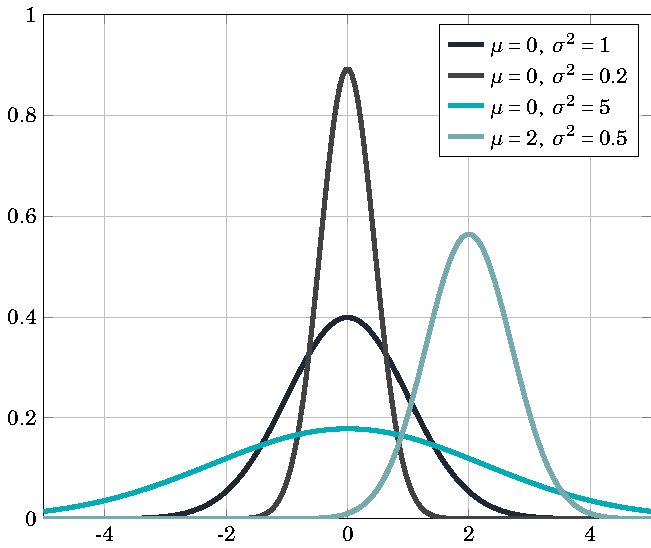
\includegraphics{ie_plot_normal.pdf}
    \caption{Gráficas de las funciones de densidad de algunas distribuciones normales.}
\end{figure}

\begin{proposition}
Si $Z \sim N(0,1)$, entonces $M_Z(t) = e^{\frac{t^2}{2}}$ para todo $t \in \R$.
\end{proposition}

\begin{proof}
En efecto,
    \[
    \begin{aligned}[t]
    M_Z(t) &= E(e^{tZ}) = \int_{\R} e^{tz}\frac{1}{\sqrt{2\pi}}e^{-\frac{z^2}{2}} \, dz = \int_{\R} \frac{1}{\sqrt{2\pi}}e^{-\frac{1}{2}(z^2-2tz)} \, dz =\int_{\R} \frac{1}{\sqrt{2\pi}}e^{-\frac{1}{2}(z^2-2tz+t^2)+\frac{1}{2}t^2} \, dz \\
    &= \int_{\R} \frac{1}{\sqrt{2\pi}}e^{-\frac{1}{2}(z-t)^2}e^{\frac{t^2}{2}} \, dz = e^{\frac{t^2}{2}}\int_{\R} \frac{1}{\sqrt{2\pi}}e^{-\frac{1}{2}(z-t)^2} \, dz \overset{(\ast)}{=} e^{\frac{t^2}{2}} \int_{\R}\frac{1}{\sqrt{2\pi}} e^{-\frac{x^2}{2}} \, dx = e^{\frac{t^2}{2}},
    \end{aligned}
    \]
    donde en $(\ast)$ se ha realizado el cambio de variable $z=t+ x$, $dz =dx $, y en la igualdad siguiente se ha usado que la integral sobre $\R$ de la función de densidad de $Z$ vale $1$.
\end{proof}

\begin{corollary}
Si $X \sim N(\mu,\sigma^2)$, entonces
\begin{enumerate}
    \item $M_X(t) = e^{\frac{1}{2}t^2\sigma^2+t\mu}$.
    \item $E(X) =\mu$.
    \item $\textup{Var}(X) = \sigma^2$.
\end{enumerate}
\end{corollary}

\begin{proof}
En efecto, usando que $Z =\frac{X-\mu}{\sigma} \sim N(0,1)$ y empleando la proposición anterior,
\[
    \begin{aligned}[t]
    M_X(t) =M_{\sigma Z+\mu}(t) = E(e^{t(\sigma Z+\mu)} ) = E(e^{t\sigma Z}) E(e^{t\mu}) = M_Z(t\sigma) e^{t\mu} = e^{\frac{1}{2}t^2\sigma^2}e^{t\mu} = e^{\frac{1}{2}t^2\sigma^2+t\mu}
    \end{aligned}
    \]
Por tanto, $E(X) = M_X'(0) = \mu$, y como $E(X^2) = M_X''(0) = \sigma^2+\mu^2$, el apartado tercero está regalado.
\end{proof}

\begin{proposition}
\label{prop2.5}
Se verifican las siguientes propiedades:
\begin{enumerate}
    \item Si $X \sim N(\mu_X,\sigma^2_X)$ e $Y \sim N(\mu_Y,\sigma^2_Y)$ son variables aleatorias independientes, entonces \[X+Y \sim N(\mu_X+\mu_Y,\sigma_X^2+\sigma_Y^2)\]
    \item Si $X \sim N(\mu,\sigma^2)$, entonces, para todo $a \in \R$, \[aX \sim N(a\mu,a^2\sigma^2)\]
\end{enumerate}
\end{proposition}

\begin{proof}
    Ejercicio.
\end{proof}

\begin{corollary}
\label{cor2.6}
Si $(X_1,\mathellipsis,X_n)$ es una muestra aleatoria simple de $X \sim N(\mu,\sigma^2)$, entonces
\[\overline{X} \sim N\bigl(\mu,\frac{\sigma^2}{n}\bigr)\]
\end{corollary}

\begin{proof}
Por el primer apartado de la proposición anterior,
\[\sum_{i=1}^n X_i \sim N\bigl(\sum_{i=1}^n \mu, \sum_{i=1}^n \sigma^2 \bigr) = N(n\mu, n\sigma^2),\]
luego
\[\overline{X}= \frac{1}{n} \sum_{i=1}^n X_i \sim N\bigl(\frac{1}{n}n\mu,\frac{1}{n^2}n\sigma^2\bigr) = N\bigl(\mu, \frac{\sigma^2}{n}\bigr),\]
donde se ha aplicado el segundo apartado de la proposición anterior.
\end{proof}

\section{Distribución gamma}

La estrecha relación de la distribución gamma con la distribución normal quedará al descubierto en la sección siguiente. Por ahora, merece la pena mencionar las propiedades básicas de esta distribución.

\begin{definition}
Dados $\alpha > 0$ y $\beta >0$, se dice que $X$ sigue una \emph{distribución gamma de parámetros $\alpha$ y $\beta$}, y se denota $X \sim Ga(\alpha,\beta)$, cuando
    \[f(x) =\begin{cases}
        \displaystyle \frac{\beta^\alpha}{\Gamma(\alpha)}x^{\alpha-1}e^{-\beta x} & $si $ x>0 \\[10pt]
        0 & $en otro caso,$
    \end{cases} \]
    donde
    \[\Gamma(\alpha)=\int_0^{+\infty} x^{\alpha-1}e^{-x} \, dx\]
    es la denominada \emph{función gamma}.
\end{definition}

\begin{figure}[H]
    \centering
    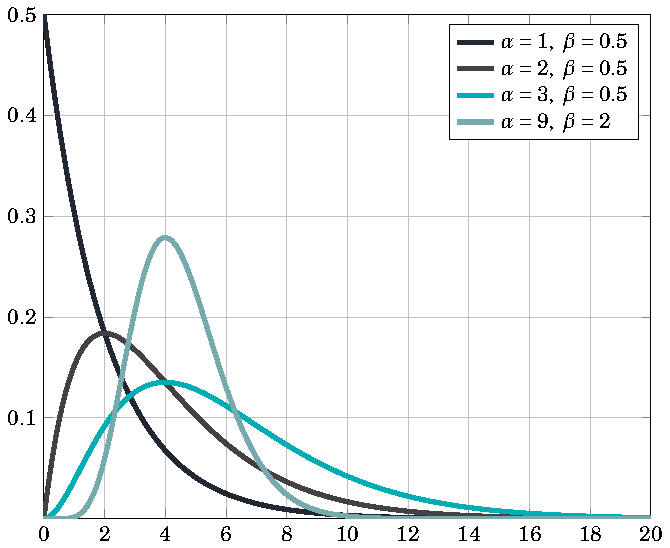
\includegraphics{ie_plot_gamma.pdf}
    \caption{Gráficas de las funciones de densidad de algunas distribuciones gamma.}
\end{figure}

\begin{proposition}
La función gamma verifica las siguientes propiedades:
\begin{enumerate}
    \item $\Gamma(z+1)=z\Gamma(z)$ para todo $z >0$.
    \item $\Gamma(n+1)=n!$ para todo $n \in \N$.
    \item $\displaystyle \Gamma\bigl(\frac{1}{2}\bigr) = \sqrt{\pi}$.
\end{enumerate}
\end{proposition}

\begin{proof}
Solo se va a demostrar el último apartado. Se tiene que \[\Gamma\bigl(\frac{1}{2}\bigr) = \int_0^\infty x^{-\frac{1}{2}}e^{-x} \, dx = \int_0^\infty \frac{e^{-x}}{\sqrt{x}} \, dx \overset{(\ast)}{=} \int_0^\infty 2e^{-y^2} \, dy = 2\frac{\sqrt{\pi}}{2} = \sqrt{\pi},\]
donde en $(\ast)$ se ha realizado el cambio de variable $x = y^2$, $dx = 2y\, dy$. \qedhere
\end{proof}

\begin{proposition}
\label{prop2.9}
Si $X \sim Ga(\alpha,\beta)$, entonces
\begin{enumerate}
    \item $\displaystyle E(X) = \frac{\alpha}{\beta}$.
    \item $\displaystyle \textup{Var}(X) = \frac{\alpha}{\beta^2}$.
    \item $\displaystyle M_X(t) = \bigl(1-\frac{t}{\beta}\bigr)^{-\alpha}$ siempre que $t < \beta$.
    \item $\displaystyle E(X^r) = \frac{\Gamma(\alpha+r)}{\Gamma(\alpha)\beta^r}$ para todo $r \in \N$.
\end{enumerate}
\end{proposition}

\begin{proof}
    Ejercicio.
\end{proof}

\begin{proposition}
\label{prop2.10}
Se verifican las siguientes propiedades:
\begin{enumerate}
    \item Si $X_1,\mathellipsis,X_n$ son variables aleatorias independientes con $X_i \sim Ga(\alpha_i,\beta)$ para cada $i \in \{1,\mathellipsis,n\}$, entonces
\[\sum_{i=1}^n X_i \sim Ga\bigl(\sum_{i=1}^n \alpha_i,\beta\bigr)\]
\item Si $X \sim Ga(\alpha,\beta)$, entonces $cX \sim Ga(\alpha,\frac{\beta}{c})$ para todo $c >0$.
\end{enumerate}
\end{proposition}

\begin{proof}
    Ejercicio.
\end{proof}

\begin{proposition}
\label{prop2.11}
    Si $Z \sim N(0,1)$, entonces
    \[Z^2 \sim Ga\bigl(\frac{1}{2},\frac{1}{2}\bigr)\]
\end{proposition}

\begin{proof}
Tenemos que, para todo $z \geq 0$,
\[\begin{aligned}[t]
F_{Z^2}(z) &= P(Z^2 \leq z) = P(|Z| \leq \sqrt{z}) = P(-\sqrt{z} \leq Z \leq \sqrt{z}) = \int_{-\sqrt{z}}^{\sqrt{z}} f_Z(t) \, dt = \int_{-\infty}^{\sqrt{z}}f_Z(t) \, dt - \int_{-\infty}^{-\sqrt{z}} f_Z(t) \, dt \\
&= F_Z(\sqrt{z})-(1-\int_{-\sqrt{z}}^\infty f_Z(t) \, dt) \overset{(\ast)}{=} F_Z(\sqrt{z})-(1-\int_{-\infty}^{\sqrt{z}} f_Z(t) \, dt) = 2F_Z(\sqrt{z})-1,
\end{aligned}
\]
donde en $(\ast)$ se ha usado que la función de densidad de $Z$ es una función par. Por tanto,
\[f_{Z^2}(z) = F_{Z^2}'(z) = 2F_Z'(\sqrt{z}) \frac{1}{2\sqrt{z}} = \frac{f_Z(\sqrt{z})}{\sqrt{z}} =\frac{1}{\sqrt{2\pi z}}e^{-\frac{z}{2}} = \frac{(\frac{1}{2})^{\frac{1}{2}}}{\Gamma(\frac{1}{2})}z^{\frac{1}{2}-1}e^{-\frac{1}{2}z},\]
lo que demuestra que $Z^2\sim Ga(\frac{1}{2},\frac{1}{2})$.
\end{proof}

\section{Distribución \texorpdfstring{$\chi^2$}{TEXT} de Pearson}

\begin{definition}
Sea $(X_1,\mathellipsis,X_n)$ una muestra aleatoria simple de $X \sim N(0,1)$. La variable aleatoria
\[V = \sum_{i=1}^n X_i^2\]
se dice que sigue una \emph{distribución $\chi^2$ con $n$ grados de libertad}, y se denota $V \sim \chi_n^2$.
\end{definition}

\begin{proposition}
    La función de densidad de $V \sim \chi^2_n$ es
    \[f_n(v) = \begin{cases}
        \displaystyle \frac{1}{2^{\frac{n}{2}}\Gamma(\frac{n}{2})}v^{\frac{n}{2}-1}e^{-\frac{v}{2}} & $ si $ v >0 \\
        0 & $ en otro caso$
    \end{cases}\]
En otras palabras, $V \sim \textup{Ga}(\frac{n}{2},\frac{1}{2})$.

\end{proposition}

\begin{proof}
    No es asunto de esta asignatura.
\end{proof}

\begin{figure}[H]
    \centering
    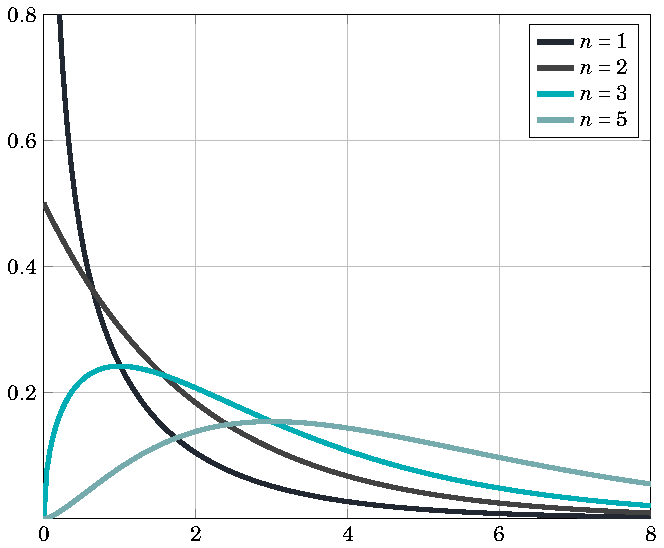
\includegraphics{ie_plot_chi.pdf}
    \caption{Gráficas de las funciones de densidad de algunas distribuciones $\chi^2_n$.}
\end{figure}

\begin{corollary}
\label{cor2.14}
Si $V \sim \chi^2_n$, entonces
\begin{enumerate}
    \item $E(V) = n$.
    \item $\textup{Var}(V) = 2n$.
    \item $\displaystyle M_V(t) = (1-2t)^{-\frac{n}{2}}$ siempre que $\displaystyle t < \frac{1}{2}$.
    \item $\displaystyle E(X^r) = \frac{2^r \Gamma(r+\frac{n}{2})}{\Gamma(\frac{n}{2})}$.
\end{enumerate}
\end{corollary}

\begin{proof}
No hay más que aplicar la proposición anterior y la \hyperref[prop2.9]{\color{blue}Proposición 13}.
\end{proof}

\begin{corollary}
Si $V_i \sim \chi^2_{n_i}$ ($i =1,\mathellipsis,k$) son variables aleatorias independientes, entonces
\[\sum_{i=1}^k V_i \sim \chi^2_{\sum_{i=1}^k n_i}\]
\end{corollary}

\begin{proof}
No hay más que aplicar la proposición anterior y la \hyperref[prop2.10]{\color{blue}Proposición 14}.
\end{proof}

\begin{corollary}
Si $X \sim N(0,1)$, entonces $X^2 \sim \chi^2_1$.
\end{corollary}

\begin{proof}
No hay más que aplicar la proposición anterior y la \hyperref[prop2.11]{\color{blue}Proposición 15}.
\end{proof}

\begin{corollary}
\label{cor2.17}
Si $(X_1,\mathellipsis,X_n)$ es una muestra aleatoria simple de $X \sim N(\mu,\sigma^2)$, entonces
    \[\sum_{i=1}^n\bigl(\frac{X_i-\mu}{\sigma}\bigr)^2 \sim \chi^2_n\]
\end{corollary}

\begin{proof}
Llamamos, para cada $i \in \{1,\mathellipsis,n\}$, $Y_i = \bigl(\frac{X_i-\mu}{\sigma}\bigr)^2$. Por el corolario anterior se tiene $Y_i\sim \chi^2_1$ para todo $i \in \{1,\mathellipsis,n\}$, luego
\[M_{\sum_{i=1}^nY_i}(t) = \prod_{i=1}^nM_{Y_i}(t)= \prod_{i=1}^n(1-2t)^{-\frac{1}{2}} = (1-2t)^{-\frac{n}{2}}\]
para todo $t < \frac{1}{2}$, de donde se deduce inmediatamente la afirmación del enunciado.
\end{proof}

\begin{corollary}
\label{cor2.18}
Si $(X_1,\mathellipsis,X_n)$ es una muestra aleatoria simple de $X \sim N(\mu,\sigma^2)$, entonces
\[\bigl(\frac{\overline{X}-\mu}{\sigma}\bigr)^2n \sim \chi^2_1\]
\end{corollary}

\begin{proof}
No hay más que aplicar el corolario anterior con $n=1$ y el \hyperref[cor2.6]{\color{blue}Corolario 2}.
\end{proof}

\section{Distribución \texorpdfstring{$t$}{TEXT} de Student}

\begin{definition}
Si $Z \sim N(0,1)$ y $V \sim \chi^2_n$ son independientes, la variable aleatoria
\[T= \frac{Z}{\sqrt{\frac{V}{n}}}\]
se dice que sigue una \emph{distribución $t$ con $n$ grados de libertad}, y se denota $T \sim t_n$.
\end{definition}

\begin{proposition}
Una variable aleatoria $T$ que sigue una distribución $t$ con $n$ grados de libertad verifica las siguientes propiedades:
\begin{enumerate}
    \item La función de densidad de $T$ es
\[f_n(t) = \frac{\Gamma(\frac{n+1}{2})}{\Gamma(\frac{n}{2})\sqrt{n\pi}}\bigl(1+\frac{t^2}{n}\bigr)^{-\frac{n+1}{2}}\]
para todo $t \in \R$.
\item Si $n>1$,
\[E(T) = 0\]
\item Si $n>2$,
\[\textup{Var}(T) = \frac{n}{n-2}\]
\end{enumerate}
\end{proposition}

\begin{proof}
    No es asunto de esta asignatura.
\end{proof}

\begin{figure}[H]
    \centering
    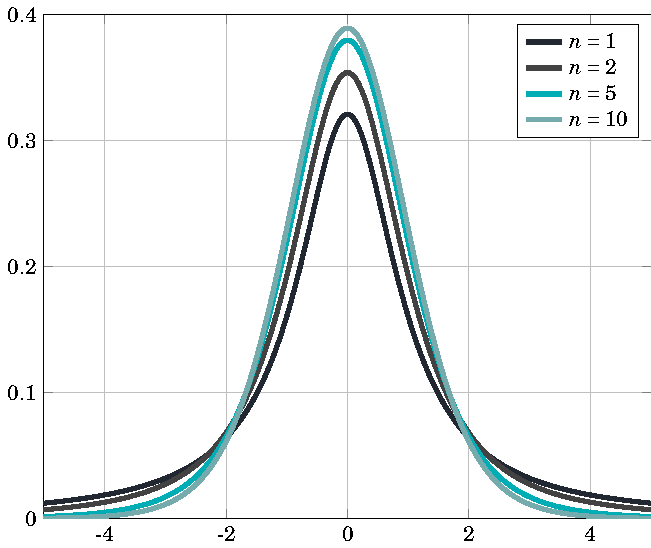
\includegraphics{ie_plot_student.pdf}
    \caption{Gráficas de las funciones de densidad de algunas distribuciones $t_n$.}
\end{figure}

\section{Distribución \texorpdfstring{$F$}{TEXT} de Snedecor}

\begin{definition}
Si $V \sim \chi^2_n$ y $W \sim \chi^2_m$ son independientes, la variable aleatoria
\[F = \frac{\frac{V}{n}}{\frac{W}{m}}\]
se dice que sigue una \emph{distribución $F$ con $n$ y $m$ grados de libertad}, y se denota $F \sim F_{n,m}$.
\end{definition}

\begin{proposition}
Una variable aleatoria $F$ que sigue una distribución $F$ con $n$ y $m$ grados de libertad verifica las siguientes propiedades:
\begin{enumerate}
\item La función de densidad de $F$ es
\[f_{n,m}(x) = \begin{cases}
    \displaystyle \frac{\Gamma(\frac{n+m}{2})}{\Gamma(\frac{n}{2})\Gamma(\frac{m}{2})}\bigl(\frac{n}{m}\bigr)^{\frac{n}{2}}x^{\frac{n}{2}-1}\bigl(1+\frac{n}{m}x\bigr)^{-\frac{n+m}{2}} & $ si $ x >0 \\
    0 & $ en otro caso$
\end{cases}
\]
\item Si $m>2$,
\[E(F)=\frac{m}{m-2}\]
\item Si $m>4$,
\[\textup{Var}(F) = \frac{2m^2(m+n-2)}{n(m-2)^2(m-4)}\]
\end{enumerate}
\end{proposition}

\begin{proof}
    No es asunto de esta asignatura.
\end{proof}

\begin{figure}[H]
    \centering
    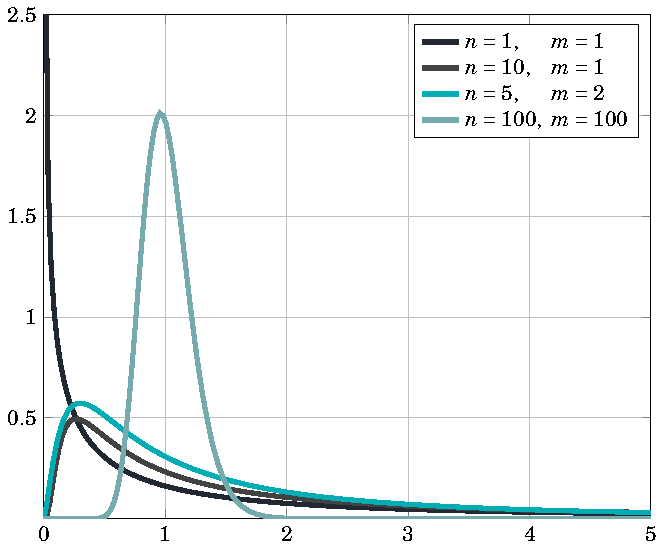
\includegraphics{ie_plot_snedecor.pdf}
    \caption{Gráficas de las funciones de densidad de algunas distribuciones $F_{n,m}$.}
\end{figure}

\section{Propiedades de la media muestral y la cuasivarianza muestral}

\begin{proposition}
Considérese una muestra aleatoria simple $(X_1,\mathellipsis,X_n)$ de $X \sim N(\mu,\sigma^2)$. Entonces $\overline{X}$ y $(X_1-\overline{X},\mathellipsis,X_n-\overline{X})$ son independientes, es decir, se verifica
\[M_{(\overline{X},X_1-\overline{X},\mathellipsis,X_n-\overline{X})}(t,t_1,\mathellipsis,t_n) = M_{\overline{X}}(t)M_{(X_1-\overline{X},\mathellipsis,X_n-\overline{X})}(t_1,\mathellipsis,t_n)\]
para todo $t \in \R$ y todo $(t_1,\mathellipsis,t_n) \in \R^n$.
\end{proposition}

\begin{proof}
Antes de empezar, dado $(t_1,\mathellipsis,t_n) \in \R^n$, será conveniente denotar \[\overline{t} = \frac{1}{n}\sum_{i=1}^n t_i\]
Se tiene que
\[
\begin{aligned}[t]
M_{(X_1-\overline{X},\mathellipsis,X_n-\overline{X})}(t_1,\mathellipsis,t_n) &= E\bigl(e^{\sum_{i=1}^n t_i(X_i-\overline{X})}\bigr) = E\bigl(e^{\sum_{i=1}^n t_iX_i-\overline{X}\sum_{i=1}^n t_i}\bigr) = E\bigl(e^{\sum_{i=1}^n t_iX_i-\overline{t}\sum_{i=1}^n X_i}\bigr) \\ &= E\bigl(e^{\sum_{i=1}^n X_i(t_i-\overline{t})}\bigr) = E\bigl(\prod_{i=1}^n e^{X_i(t_i-\overline{t})}\bigr) = \prod_{i=1}^nE\bigl(e^{X_i(t_i-\overline{t})}\bigr) = \prod_{i=1}^n M_{X_i}(t_i-\overline{t})
\end{aligned}
\]
Además,
\[M_{\overline{X}}(t) = E(e^{t\overline{X}}) = E\bigl(e^{\sum_{i=1}^n \frac{t}{n}X_i}\bigr) = E\bigl(\prod_{i=1}^n e^{\frac{t}{n}X_i}\bigr) = \prod_{i=1}^n E(e^{\frac{t}{n}X_i}) = \prod_{i=1}^n M_{X_i}\bigl(\frac{t}{n}\bigr) = \prod_{i=1}^n e^{\frac{1}{2}\frac{t^2}{n^2}\sigma^2+\frac{t}{n}\mu} = e^{\frac{1}{2}\frac{t^2}{n}\sigma^2+t\mu}\]
Por otro lado,
\[\begin{aligned}[t]
    M_{(\overline{X},X_1-\overline{X},\mathellipsis,X_n-\overline{X})}(t,t_1,\mathellipsis,t_n) &= E\bigl(e^{t\overline{X}+\sum_{i=1}^n t_i(X_i-\overline{X})}\bigr) = E\bigl(e^{t\overline{X}+\sum_{i=1}^n t_iX_i-\sum_{i=1}^n t_i\overline{X})}\bigr) \\
    &= E\bigl(e^{\sum_{i=1}^n t_iX_i-\overline{X}(\sum_{i=1}^nt_i-t)}\bigr) = E\bigl(e^{\sum_{i=1}^n X_i(t_i-\frac{1}{n}(\sum_{i=1}^nt_i-t))}\bigr) \\ 
    &= E\bigl(\prod_{i=1}^n e^{X_i(t_i-\frac{1}{n}(\sum_{i=1}^nt_i-t))}\bigr) =\prod_{i=1}^n E\bigl(e^{X_i(t_i-\frac{1}{n}(\sum_{i=1}^nt_i-t))}\bigr) \\ 
    &= \prod_{i=1}^n E\bigl(e^{X_i(t_i-\overline{t}+\frac{t}{n})}\bigr) = \prod_{i=1}^n E\bigl(e^{X_i(t_i-\overline{t})}e^{X_i\frac{t}{n}}\bigr) = \prod_{i=1}^n E(e^{X_i(t_i-\overline{t})}) E(e^{X_i\frac{t}{n}}) \\
    &= \prod_{i=1}^n M_{X_i}(t_i-\overline{t}) M_{X_i}\bigl(\frac{t}{n}\bigr) = \prod_{i=1}^n M_{X_i}(t_i-\overline{t}) e^{\frac{1}{2}\frac{t^2}{n^2}\sigma^2+\frac{t}{n}\mu} \\
    &= e^{\frac{1}{2}\frac{t^2}{n}\sigma^2+t\mu}\prod_{i=1}^n M_{X_i}(t_i-\overline{t}),
\end{aligned}\]
así que se verifica la igualdad del enunciado.
\end{proof}

\begin{proposition}[Lema de Fisher]
\label{prop20}
Sea $(X_1,\mathellipsis,X_n)$ una muestra aleatoria simple de $X \sim N(\mu,\sigma^2)$. Entonces
\begin{enumerate}
    \item $\overline{X}$ y $S_c^2$ son variables aleatorias independientes.
    \item $\displaystyle \overline{X} \sim N\bigl(\mu, \frac{\sigma^2}{n}\bigr)$.
    \item $\displaystyle \frac{(n-1)S_c^2}{\sigma^2} \sim \chi^2_{n-1}$.
    \item $\displaystyle \frac{(\overline{X}-\mu)\sqrt{n}}{\sqrt{S_c^2}} \sim t_{n-1}$
\end{enumerate} 
\end{proposition}

\begin{proof}

\hfill

\begin{enumerate}
    \item Considérese la función $g \colon \R^n \to \R$ dada por
    \[g(t_1,\mathellipsis,t_n) = \frac{1}{n-1} \sum_{i=1}^n t_i^2\]
    Como $\overline{X}$ e $Y = (X_1-\overline{X},\mathellipsis,X_n-\overline{X})$ son independientes y $g$ es continua, entonces $\overline{X}$ y $g(Y) = S^2_c$ también son independientes.
    \item Como $X_i \sim N(\mu,\sigma^2)$ para todo $i \in \{1,\mathellipsis,n\}$, entonces
    \[\sum_{i=1}^n X_i \sim N\bigl(\sum_{i=1}^n \mu, \sum_{i=1}^n \sigma^2\bigr) = N(n\mu, n\sigma^2),\]
    luego, empleando la \hyperref[prop2.5]{\color{blue}Proposición 11},
    \[\overline{X} = \frac{1}{n}\sum_{i=1}^n X_i \sim N\bigl(\mu,\frac{\sigma^2}{n}\bigr),\]
    \item Nótese que
    \[U = \frac{(n-1)S^2_c}{\sigma^2} = \frac{nS^2}{\sigma^2} = \sum_{i=1}^n\frac{(X_i-\overline{X})^2}{\sigma^2}\]
    Se sabe, por el \hyperref[cor2.17]{\color{blue}Corolario 6}, que 
    \[V = \sum_{i=1}^n\bigl(\frac{X_i-\mu}{\sigma}\bigr)^2  \sim \chi^2_n\]
    Pero
    \[
    \begin{aligned}[t]
    V &=\sum_{i=1}^n\frac{ (X_i-\overline{X}+\overline{X}-\mu)^2}{\sigma^2}= \sum_{i=1}^n\frac{(X_i-\overline{X})^2}{\sigma^2}+\sum_{i=1}^n \frac{(\overline{X}-\mu)^2}{\sigma^2}+\cancel{\frac{2(\overline{X}-\mu)}{\sigma^2}\sum_{i=1}^n(X_i-\overline{X})} \\ &= \sum_{i=1}^n\frac{(X_i-\overline{X})^2}{\sigma^2}+\bigl(\frac{\overline{X}-\mu}{\sigma}\bigr)^2n = U+W
    \end{aligned}
    \]
    El \hyperref[cor2.18]{\color{blue}Corolario 7} también permite afirmar que $W \sim \chi^2_1$. Por tanto, por el \hyperref[cor2.14]{\color{blue}Corolario 3},
    \[M_V(t) = (1-2t)^{-\frac{n}{2}} \qquad \textup{y} \qquad M_W(t) = (1-2t)^{-\frac{1}{2}}\]
    para todo $t < \frac{1}{2}$. Así, usando que $U$, $V$ y $W$ son independientes,
    \[M_U(t) = M_{V-W}(t)=\frac{M_V(t)}{M_W(t)} = (1-2t)^{-\frac{n}{2}+\frac{1}{2}} = (1-2t)^{-\frac{n-1}{2}}\]
    Se concluye que $U \sim \chi^2_{n-1}$.
    \item Por $(ii)$ y por $(iii)$, respectivamente,
    \[Z=\frac{(\overline{X}-\mu)\sqrt{n}}{\sigma} \sim N(0,1) \qquad \textup{y} \qquad V=\frac{(n-1)S^2_c}{\sigma^2}\sim \chi^2_{n-1}\]
    Por tanto,
    \[\frac{Z}{\sqrt{\frac{V}{n-1}}} = \frac{\sqrt{n-1}\frac{(\overline{X}-\mu)\sqrt{n}}{\sigma}}{\sqrt{{\frac{(n-1)S^2_c}{\sigma^2}}}} = \frac{\frac{(\overline{X}-\mu)\sqrt{n}}{\sigma}}{\frac{\sqrt{S^2_c}}{\sigma}} = \frac{(\overline{X}-\mu)\sqrt{n}}{\sqrt{S^2_c}} \sim t_{n-1},\]
    teniéndose en cuenta que $Z$ y $V$ son independientes por serlo $\overline{X}$ y $S^2_c$, como se probó en el apartado primero. \qedhere
\end{enumerate}
    
\end{proof}

\begin{corollary}
\label{cor8}
Sea $(X_1,\mathellipsis,X_n)$ una muestra aleatoria simple de $X \sim N(\mu_X,\sigma_X^2)$ y sea $(Y_1,\mathellipsis,Y_m)$ una muestra aleatoria simple de $Y \sim N(\mu_Y,\sigma_Y^2)$, siendo $X$ e $Y$ variables aleatorias independientes. Entonces
\begin{enumerate}
    \item $\displaystyle \frac{S_{c,X}^2\sigma^2_Y}{S^2_{c,Y}\sigma^2_X} \sim F_{n-1,m-1}$
    \item $\displaystyle \sqrt{\frac{n+m-2}{\frac{\sigma^2_X}{n}+\frac{\sigma^2_Y}{m}}}\frac{\overline{X}-\overline{Y}-(\mu_X-\mu_Y)}{\sqrt{\frac{(n-1)S_{c,X}^2}{\sigma^2_X}+\frac{(m-1)S_{c,Y}^2}{\sigma^2_Y}}} \sim t_{n+m-2}$
\end{enumerate}
\end{corollary}

\begin{proof}
\hfill
\begin{enumerate}
    \item Se tiene que
    \[\frac{S^2_{c,X}\sigma^2_Y}{S^2_{c,Y}\sigma^2_X} = \frac{\frac{(n-1)S^2_{c,X}}{\sigma^2_X}}{\frac{(m-1)S^2_{c,Y}}{\sigma^2_Y}}\frac{m-1}{n-1} = \frac{\frac{V}{n-1}}{\frac{W}{m-1}} \sim F_{n-1,m-1}\]
    Se ha usado que, por el lema de Fisher, $V \sim \chi^2_{n-1}$ y $W \sim \chi^2_{m-1}$.
    \item Por el lema de Fisher, se sabe que
    \[\overline{X} \sim N\bigl(\mu_X,\frac{\sigma^2_X}{n}\bigr) \qquad \textup{y} \qquad \overline{Y} \sim N\bigl(\mu_Y,\frac{\sigma^2_Y}{m}\bigr)\]
    Por tanto,
    \[\overline{X}-\overline{Y} \sim N\bigl(\mu_X-\mu_Y,\frac{\sigma^2_X}{n}+\frac{\sigma^2_Y}{m}\bigr)\]
    En consecuencia,
    \[Z=\frac{\overline{X}-\overline{Y}-(\mu_X-\mu_Y)}{\sqrt{\frac{\sigma^2_X}{n}+\frac{\sigma^2_Y}{m}}} \sim N(0,1)\]
    Además, también por el lema de Fisher,
    \[\frac{(n-1)S^2_{c,X}}{\sigma^2_X} \sim \chi^2_{n-1} \qquad \textup{y} \qquad \frac{(m-1)S^2_{c,Y}}{\sigma^2_Y} \sim \chi^2_{m-1}\]
    Así,
    \[V= \frac{(n-1)S^2_{c,X}}{\sigma^2_X}+\frac{(m-1)S^2_{c,Y}}{\sigma^2_Y} \sim \chi^2_{n-1+m-1} = \chi^2_{n+m-2}\]
    Total, que se tiene
    \[\frac{Z}{\sqrt{\frac{V}{n+m-2}}} \sim t_{n+m-2}\]
    Si se compara esta variable aleatoria con la del enunciado, no queda nada que probar. \qedhere
\end{enumerate}
\end{proof}

\chapter{Estimación puntual paramétrica}

Considérese una variable aleatoria $X$ cuya función de distribución depende de un cierto parámetro $\theta$ desconocido, del que solo se sabe que pertene a un cierto espacio paramétrico $\Theta$. El objetivo de este tema consistirá en estimar este parámetro $\theta$. Para ello, serán de cierta utilidad los estadísticos muestrales, pues el hecho de conocer, por ejemplo, la media o la varianza de una muestra aleatoria simple de $X$ permitirá obtener cierta información del parámetro $\theta$.

En gran parte del tema será necesario referirse a la función de masa o densidad de $X$ dependiendo de si es discreta o absolutamente continua. Para facilitar la escritura y no tener que distinguir entre función de masa y de densidad constantemente, será frecuente denotar por $f_\theta$ a ambas.

\section{Función de verosimilitud}

\begin{definition}
Sea $X$ una variable aleatoria con función de masa o densidad $f_\theta$, donde $\theta$ pertenece a un espacio paramétrico $\Theta$, y sea $(X_1,\mathellipsis,X_n)$ una muestra aleatoria simple de $X$. La \emph{función de verosimilitud de $(X_1,\mathellipsis,X_n)$} es la función $L \colon \chi^n \times \Theta \to \R$ dada por
\[L(x_1,\mathellipsis,x_n;\theta)=\prod_{i=1}^n f_\theta(x_i)\]
\end{definition}

Si $g_\theta$ es la función de masa o densidad del vector aleatorio $(X_1,\mathellipsis,X_n)$, usando la independencia de estas $n$ variables aleatorias puede probarse que
\[g_\theta(x_1,\mathellipsis,x_n) = \prod_{i=1}^nf_\theta(x_i), \quad (x_1,\mathellipsis,x_n) \in \R^n\]
Si a esto se le suma la costumbre de denotar de la misma manera a la función de masa o densidad de $(X_1,\mathellipsis,X_n)$ y a la de $X$, queda justificada la expresión
\[L(x_1,\mathellipsis,x_n;\theta) = f_\theta(x_1,\mathellipsis,x_n), \qquad (x_1,\mathellipsis,x_n;\theta) \in \chi^n \times \Theta\]

\begin{example}
Defínase la variable aleatoria
\[X \equiv \begin{cases}
    1 & $ si un alumno duerme menos de 6 horas$ \\
    0 & $ en otro caso$
\end{cases}\]
Si $p$ es la probabilidad de que un alumno duerma menos de $6$ horas, se tiene $X \sim Ber(p)$. Sea \[(x_1,x_2,x_3,x_4,x_5,x_6,x_7,x_8,x_9,x_{10}) = (0,0,0,0,0,1,0,0,0,0) \in \chi^{10}\] Entonces
\[L(x_1,x_2,x_3,x_4,x_5,x_6,x_7,x_8,x_9,x_{10};p) = \prod_{i=1}^{10}P_p(X = x_i) = p(1-p)^9\]
\end{example}

\section{Estadísticos suficientes}

\begin{definition}
Sea $X$ una variable aleatoria con función de masa o densidad $f_\theta$, sea $(X_1,\mathellipsis,X_n)$ una muestra aleatoria simple de $X$ y sea $T \colon \R^n \to \R$ un estadístico muestral. Se dice que $T$ es un \emph{estadístico suficiente para $\theta$} si para cada $(x_1,\mathellipsis,x_n) \in \chi^n$, el cociente
    \[\frac{f_\theta(x_1,\mathellipsis,x_n)}{g_\theta(T(x_1,\mathellipsis,x_n))} \]
    no depende de $\theta$, donde $g_\theta$ es la función de masa o densidad de la variable aleatoria $T(X_1,\mathellipsis,X_n)$.
\end{definition}

Nótese que, en el caso discreto,
\[\begin{aligned}[t]
\frac{p_\theta(x_1,\mathellipsis,x_n)}{q_\theta(T(x_1,\mathellipsis,x_n))}  &= \frac{P_\theta(X_1=x_1,\mathellipsis,X_n=x_n)}{P_\theta(T(X_1,\mathellipsis,X_n) = T(x_1,\mathellipsis,x_n))} \\
&= \frac{P_\theta(X_1=x_1,\mathellipsis,X_n=x_n,T(X_1,\mathellipsis,X_n) = T(x_1,\mathellipsis,x_n))}{P_\theta(T(X_1,\mathellipsis,X_n) = T(x_1,\mathellipsis,x_n))} \\
&=P_\theta(X_1=x_1,\mathellipsis,X_n=x_n \, \big| \, T(X_1,\mathellipsis,X_n) = T(x_1,\mathellipsis,x_n))
\end{aligned}
\]
Es por esto que será habitual emplear la notación
\[\frac{p_\theta(x_1,\mathellipsis,x_n)}{q_\theta(T(x_1,\mathellipsis,x_n))} \equiv P(X_1=x_1,\mathellipsis,X_n=x_n \, \big| \, T=t)\]

\begin{example}
Sea $X \sim Ber(p)$ y sea $(X_1,X_2,X_3)$ una muestra aleatoria simple de $X$. Considérense los estadísticos muestrales
\[T_1(X_1,X_2,X_3) = \sum_{i=1}^3 X_i, \qquad T_2(X_1,X_2,X_3) = \max\{X_1,X_2,X_3\}\]
Recogemos en una tabla los valores que pueden tomar $(X_1,X_2,X_3), T_1$ y $T_2$ con probabilidad positiva.

\begin{center}
\begin{tabular}{|c|c|c|}
\hline
     $\bm{(X_1,X_2,X_3)}$ & $\bm{T_1}$ & $\bm{T_2}$  \\ \hline
     $(0,0,0)$ & $0$ & $0$ \\
     $(1,0,0)$ & $1$ & $1$ \\
     $(0,1,0)$ & $1$ & $1$ \\
     $(0,0,1)$ & $1$ & $1$ \\
     $(1,1,0)$ & $2$ & $1$ \\
     $(0,1,1)$ & $2$ & $1$ \\
     $(1,0,1)$ & $2$ & $1$ \\
     $(1,1,1)$ & $3$ & $1$ \\ \hline
\end{tabular}
\end{center}

Veamos si $T_1$ es un estadístico suficiente. Se tiene que
\[
\begin{alignedat}{3}
    P(X_1=0,X_2=0,X_3=0 \, \big| \, T_1 = 0) &= 1,\phantom{\frac{1}{3}} & \qquad \qquad P(X_1=1,X_2=1,X_3=0 \, \big| \, T_1 = 2) &= \frac{1}{3}, \\[5pt]
    P(X_1=1,X_2=0,X_3=0 \, \big| \, T_1 = 1) &= \frac{1}{3}, & \qquad \qquad P(X_1=0,X_2=1,X_3=1 \, \big| \, T_1 = 2) &= \frac{1}{3}, \\[5pt]
    P(X_1=1,X_2=1,X_3=0 \, \big| \, T_1 = 1) &= \frac{1}{3}, & \qquad \qquad P(X_1=1,X_2=0,X_3=1 \, \big| \, T_1 = 2) &= \frac{1}{3}, \\[5pt]
    P(X_1=1,X_2=0,X_3=1 \, \big| \, T_1 = 1) &= \frac{1}{3}, & \qquad \qquad P(X_1=1,X_2=1,X_3=1 \, \big| \, T_1 = 3) &= 1,\phantom{\frac{1}{3}} \\[5pt]
\end{alignedat}
\]
y como esto no depende de $p$, entonces $T_1$ es un estadístico suficiente. Sin embargo, $T_2$ no lo es, ya que
\[P(X_1=1,X_2=0,X_3=0 \, \big| \, T_2 = 1) = \frac{p(1-p)^2}{1-(1-p)^3}\]
\end{example}

\begin{example}
Sean $X \sim P(\lambda)$ y $(X_1,\mathellipsis,X_n)$ una muestra aleatoria simple de $X$. Se considera el estadístico muestral
\[T=\sum_{i=1}^nX_i\]
Veamos si $T$ es un estadístico suficiente para $\lambda$. Si $(x_1,\mathellipsis,x_n) \in (\N \cup \{0\})^n$,
\[P(X_1=x_1,\mathellipsis,X_n=x_n \, \big| \, T=t) = \frac{P(X_1=x_1,\mathellipsis,X_n=x_n, T=t)}{P(T=t)}\]
Se tiene que
\[P(X_1=x_1,\mathellipsis,X_n=x_n, T=t) = \prod_{i=1}^n e^{-\lambda} \frac{\lambda^{x_i}}{x_i!} = e^{-n\lambda}\frac{\lambda^{\sum_{i=1}^n x_i}}{\prod_{i=1}^n x_i!}= e^{-n\lambda}\frac{\lambda^t}{\prod_{i=1}^nx_i!}\]
Por otro lado, usando que $T \sim P(n\lambda)$ por ser $X_i$ variables aleatorias independientes con $X_i \sim P(\lambda)$,
\[P(T=t) = e^{-n\lambda}\frac{(n\lambda)^t}{t!} \]
En consecuencia,
\[P(X_1=x_1,\mathellipsis,X_n=x_n \, \big| \, T=t) = \frac{t!}{n^t\prod_{i=1}^nx_i!}\]
Como esto no depende de $\lambda$, se tiene que $T$ es un estadístico suficiente para $\lambda$.
\end{example}

\begin{theorem}[Teorema de factorización de Fisher-Neyman]
Un estadístico muestral $T$ es suficiente para $\theta \in \Theta$ si y solo si existen funciones $g \colon T(\chi^n) \times \Theta \to \R$, $h \colon \chi^n \to \R$ no negativas tales que 
\[L(x_1,\mathellipsis,x_n;\theta) = g(T(x_1,\mathellipsis,x_n);\theta)h(x_1,\mathellipsis,x_n)\]
para todo $(x_1,\mathellipsis,x_n) \in \chi^n$.
\end{theorem}

\begin{proof}
Solo se va a probar para el caso discreto. Sea $T$ un estadístico suficiente para $\theta$. Entonces
\[L(x_1,\mathellipsis,x_n;\theta) = P_\theta(X_1=x_1,\mathellipsis,X_n=x_n) =P_\theta(X_1=x_1,\mathellipsis,X_n = x_n \, \big| \, T=t)P_\theta(T=t),\]
donde $t = T(x_1,\mathellipsis,x_n)$. Basta considerar
\[h(x_1,\mathellipsis,x_n) = P_\theta(X_1=x_1,\mathellipsis,X_n = x_n \, \big| \, T=t), \qquad \qquad g(t,\theta) = P(T=t),\]
que son funciones no negativas (nótese que $h$ está bien definida porque $T$ es suficiente para $\theta$). Para el recíproco, supóngase que
\[L(x_1,\mathellipsis,x_n;\theta) = g(t;\theta)h(x_1,\mathellipsis,x_n)\]
con $h$ y $g$ no negativas. Dado $t\in T(\chi^n)$, consideremos $A_t = \left\{(y_1,\mathellipsis,y_n) \in \chi^n \colon T(y_1,\mathellipsis,y_n) = t\right\}$. Entonces se tiene
\[P_\theta(T=t) = P_\theta((X_1,\mathellipsis,X_n) \in A_t) = \sum_{(y_1,\mathellipsis,y_n) \in A_t} p_\theta(y_1,\mathellipsis,y_n) = \sum_{(y_1,\mathellipsis,y_n) \in A_t} g(T(y_1,\mathellipsis,y_n);\theta)h(y_1,\mathellipsis,y_n)\]
Por otra parte,
\[
\begin{aligned}[t]
P_\theta(X_1=x_1,\mathellipsis,X_n=x_n,T=t) &= P_\theta(X_1=x_1,\mathellipsis,X_n=x_n,T(X_1,\mathellipsis,X_n)=T(x_1,\mathellipsis,x_n)) \\
&=P_\theta(X_1=x_1,\mathellipsis,X_n=x_n) \\
&= L(x_1,\mathellipsis,x_n;\theta) \\
&= g(t;\theta)h(x_1,\mathellipsis,x_n)
\end{aligned}
\]
En consecuencia,
\[\begin{aligned}[t]
P_\theta(X_1=x_1,\mathellipsis,X_n=x_n \, \big| \, T = t) &= \frac{P_\theta(X_1=x_1,\mathellipsis,X_n=x_n,T=t)}{P_\theta(T=t)} \\
&= \frac{ g(t;\theta)h(x_1,\mathellipsis,x_n)}{ g(t;\theta)\sum_{(y_1,\mathellipsis,y_n) \in A_t} h(y_1,\mathellipsis,y_n)} \\
&=\frac{h(x_1,\mathellipsis,x_n)}{\sum_{(y_1,\mathellipsis,y_n) \in A_t} h(y_1,\mathellipsis,y_n)}
\end{aligned} \]
Como esta expresión no depende de $\theta$, se concluye que $T$ es suficiente para $\theta$.
\end{proof}

\begin{example}
Sea $X \sim N(\mu,\sigma^2)$ (con $\sigma^2$ un valor conocido) y sea $(X_1,\mathellipsis,X_n)$ una muestra aleatoria simple de $X$. Considérese el estadístico muestral
\[T= \sum_{i=1}^n X_i\]
Entonces, para cada $(x_1,\mathellipsis,x_n) \in \R^n$,
\[
\begin{aligned}[t]
L(x_1,\mathellipsis,x_n;\mu) &=\prod_{i=1}^n\frac{1}{\sqrt{2\pi\sigma^2}}e^{-\frac{(x_i-\mu)^2}{2\sigma^2}} 
\\ &= \frac{1}{\left(\sqrt{2\pi\sigma^2}\right)^n}e^{-\frac{1}{2\sigma^2}\sum_{i=1}^n (x_i-\mu)^2} \\ &= \frac{1}{\left(\sqrt{2\pi\sigma^2}\right)^n}e^{-\frac{1}{2\sigma^2}\sum_{i=1}^n x_i^2}e^{-\frac{1}{2\sigma^2}\left(n\mu^2-2\mu\sum_{i=1}^n x_i\right)} \\
&= \frac{1}{\left(\sqrt{2\pi\sigma^2}\right)^n}e^{-\frac{1}{2\sigma^2}\sum_{i=1}^n x_i^2}e^{-\frac{1}{2\sigma^2}\left(n\mu^2-2\mu t\right)} \\
&= h(x_1,\mathellipsis,x_n)g(t;\mu),
\end{aligned}
\]
donde
\[h(x_1,\mathellipsis,x_n) = \frac{1}{\left(\sqrt{2\pi\sigma^2}\right)^n}e^{-\frac{1}{2\sigma^2}\sum_{i=1}^n x_i^2} \qquad \textup{y} \qquad g(t;\mu) = e^{-\frac{1}{2\sigma^2}\left(n\mu^2-2\mu t\right)} \]
son funciones no negativas. Por tanto, $T$ es un estadístico suficiente para $\mu$.
\end{example}

\begin{example}
Sean $X \sim P(\lambda)$ y $(X_1,\mathellipsis,X_n)$ una muestra aleatoria simple de $X$. Considérese el estadístico muestral
\[T = \sum_{i=1}^n X_i\]
Entonces, para cada $(x_1,\mathellipsis,x_n) \in (\N \cup \{0\})^n$,
\[
\begin{aligned}[t]
L(x_1,\mathellipsis,x_n;\lambda) &= \prod_{i=1}^n e^{-\lambda}\frac{\lambda^{x_i}}{x_i!} = e^{-n\lambda}\frac{\lambda^{\sum_{i=1}^n x_i}}{\prod_{i=1}^n x_i!} =e^{-n\lambda}\frac{\lambda^{t}}{\prod_{i=1}^n x_i!} = h(x_1,\mathellipsis,x_n)g(t,\lambda),
\end{aligned}
\]
donde
\[h(x_1,\mathellipsis,x_n) =\frac{1}{\prod_{i=1}^n x_i!} \qquad \textup{y} \qquad g(t;\lambda) = e^{-n\lambda}\lambda^t\]
son funciones no negativas. Por tanto, $T$ es un estadístico suficiente para $\lambda$.
\end{example}

\section{Estadísticos conjuntamente suficientes}

Hasta ahora se ha trabajado con estadísticos que toman valores en $\R$ y con variables aleatorias cuya función de masa o densidad depende de un parámetro unidimensional $\theta \in \R$. El objetivo de esta sección es generalizar los estadísticos suficientes al caso multidimensional. Esto resultará útil en la práctica cuando, por ejemplo, se trabaje con distribuciones normales cuya media y varianza sean desconocidas.

\begin{definition}
Sea $X$ una variable aleatoria con función de masa o densidad $f_\theta$, donde $\theta \in \R^m$. Sea $(X_1,\mathellipsis,X_n)$ una muestra aleatoria simple de $X$ y sea $T\colon \R^n \to \R^k$ un estadístico muestral. Se dice que $T$ es un \emph{estadístico conjuntamente suficiente para $\theta$} si para cada $(x_1,\mathellipsis,x_n) \in \chi^n$, el cociente
\[\frac{f_\theta(x_1,\mathellipsis,x_n)}{g_\theta(T(x_1,\mathellipsis,x_n))} \]
es independiente de $\theta$, donde $g_\theta$ es la función de masa o densidad del vector aleatorio $k$-dimensional $T(X_1,\mathellipsis,X_n)$.
\end{definition}

\begin{theorem}
Un estadístico $T \colon \R^n \to \R^k$ es conjuntamente suficiente para $\theta \in \Theta \subset \R^m$ si y solo si existen funciones $g \colon T(\chi^n) \times \Theta \to \R$, $h \colon \chi^n \to \R$ no negativas tales que para todo $(x_1,\mathellipsis,x_n) \in \chi^n$ se verifica
\[L(x_1,\mathellipsis,x_n;\theta_1,\mathellipsis,\theta_m) = g(t_1,\mathellipsis,t_k;\theta_1,\mathellipsis,\theta_m)h(x_1,\mathellipsis,x_n),\]
donde $t_i = T_i(x_1,\mathellipsis,x_n)$ para cada $i \in \{1,\mathellipsis,k\}$.
\end{theorem}

\begin{proof}
    Análoga a la del teorema anterior.
\end{proof}

\begin{example}
Sea $X \sim N(\mu,\sigma^2)$, sea $(X_1,\mathellipsis,X_n)$ una muestra aleatoria simple de $X$ y considérese el estadístico muestral $(T_1,T_2)$, donde
\[T_1 = \sum_{i=1}^n X_i, \qquad \qquad T_2 = \sum_{i=1}^nX_i^2\]
Veamos que $(T_1,T_2)$ es conjuntamente suficiente para $(\mu,\sigma^2)$. En efecto, si $(x_1,\mathellipsis,x_n) \in \R^n$,
\[
\begin{aligned}[t]
L(x_1,\mathellipsis,x_n;\mu,\sigma^2) &=\prod_{i=1}^n\frac{1}{\sqrt{2\pi\sigma^2}}e^{-\frac{(x_i-\mu)^2}{2\sigma^2}} 
\\ &= \frac{1}{\left(\sqrt{2\pi\sigma^2}\right)^n}e^{-\frac{1}{2\sigma^2}\sum_{i=1}^n (x_i-\mu)^2} \\ &= \frac{1}{\left(\sqrt{2\pi}\right)^n}\frac{1}{\sigma^n}e^{-\frac{1}{2\sigma^2}\left(\sum_{i=1}^n x_i^2+n\mu^2-2\mu\sum_{i=1}^n x_i\right)} \\
&= \frac{1}{\left(\sqrt{2\pi}\right)^n}\frac{1}{\sigma^n}e^{-\frac{1}{2\sigma^2}\left(t_2+n\mu^2-2\mu t_1\right)} \\
&= h(x_1,\mathellipsis,x_n)g(t_1,t_2;\mu,\sigma^2),
\end{aligned}
\]
donde
\[h(x_1,\mathellipsis,x_n) = \frac{1}{\left(\sqrt{2\pi}\right)^n}, \qquad \qquad g(t_1,t_2;\mu,\sigma^2) = \frac{1}{\sigma^n}e^{-\frac{1}{2\sigma^2}\left(t_2+n\mu^2-2\mu t_1\right)},\]
son funciones no negativas.
\end{example}

\begin{proposition}
Sean $X$ una variable aleatoria y $(X_1,\mathellipsis,X_n)$ una muestra aleatoria simple de $X$.
\begin{enumerate}
    \item Si $T_i=X_i$, $i \in \{1,\mathellipsis,n\}$, entonces el estadístico $(T_1,\mathellipsis,T_n)$ es conjuntamente suficiente para $\theta$.
    \item Si $T_i = X_{(i)}$, $i \in \{1,\mathellipsis,n\}$, entonces el estadístico $(T_1,\mathellipsis,T_n)$ es conjuntamente suficiente para $\theta$.
\end{enumerate}
\end{proposition}
\begin{proof}
    Ejercicio.
\end{proof}

\section{Familia exponencial uniparamétrica}

\begin{definition}
Sea $X$ una variable aleatoria con función de masa o densidad $f_\theta$, donde $\theta \in \Theta \subset \R$. Se dice que \emph{$f_\theta$ pertenece a una familia exponencial uniparamétrica} si existen funciones $a, c \colon \Theta \to \R$, $b,d \colon \chi \to \R$, con $a$ y $b$ son no negativas, tales que para cada $x \in \chi$ se verifica
\[f_\theta(x) = a(\theta) b(x)e^{c(\theta)d(x)}\]
\end{definition}

\begin{proposition}
Sea $X$ una variable aleatoria cuya función de masa o densidad $f_\theta$ pertenece a una familia exponencial uniparamétrica. Si $(X_1,\mathellipsis,X_n)$ es una muestra aleatoria simple de $X$, entonces
\[T=\sum_{i=1}^n d(X_i)\]
es un estadístico muestral suficiente para $\theta$.
\end{proposition}

\begin{proof}
Se tiene que
\[L(x_1,\mathellipsis,x_n;\theta) = \prod_{i=1}^n f_\theta(x_i) = a(\theta)^ne^{c(\theta)\sum_{i=1}^n d(x_i)}\prod_{i=1}^nb(x_i) = a(\theta)^ne^{c(\theta)t}\prod_{i=1}^nb(x_i) = g(t;\theta)h(x_1,\mathellipsis,x_n), \]
donde \[h(x_1,\mathellipsis,x_n) = \prod_{i=1}^n b(x_i),\qquad\qquad g(t;\theta)= a(\theta)^n e^{c(\theta)t}\]
son funciones no negativas.
\end{proof}

\begin{example}
Sea $X \sim P(\lambda)$, sea $(X_1,\mathellipsis,X_n)$ una muestra aleatoria simple de $X$ y sea
\[T=\sum_{i=1}^nX_i\]
Dado $x \in \N \cup \{0\}$, se tiene que
\[P_\lambda(X=x) = e^{-\lambda} \frac{\lambda^x}{x!} =e^{-\lambda}\frac{e^{x\log(\lambda)}}{x!} =a(\lambda)b(x)e^{c(\lambda)d(x)},\]
donde
\[a(\lambda) =e^{-\lambda}, \qquad b(x)=\frac{1}{x!}, \qquad c(\lambda) =\log(\lambda), \qquad d(x)= x,\]
siendo $a, c \colon (0,\infty) \to \R$, $b,d\colon \N \cup \{0\} \to \R$ con $a$ y $b$ no negativas. Por la proposición anterior, $T$ es un estadístico suficiente para $\theta$.
\end{example}

\section{Familia exponencial \texorpdfstring{$k$}{TEXT}-paramétrica}

\begin{definition}
Sea $X$ una variable aleatoria con función de masa o densidad $f_\theta$, donde $\theta \in \Theta \subset \R^k$. Se dice que \emph{$f_\theta$ pertenece a una familia exponencial $k$-paramétrica} si existen funciones $a, c_i \colon \Theta \to \R$, $b,d_i \colon \chi \to \R$, con $a$ y $b$ no negativas e $i \in \{1,\mathellipsis,k\}$, tales que para cada $x \in \chi$ se verifica
\[f_\theta(x) = a(\theta_1,\mathellipsis,\theta_k) b(x)e^{\sum_{i=1}^kc_i(\theta_1,\mathellipsis,\theta_k)d_i(x)}\]

\end{definition}

\begin{proposition}
Sea $X$ una variable aleatoria cuya función de masa o densidad $f_\theta$ pertenece a una familia exponencial $k$-paramétrica. Si $(X_1,\mathellipsis,X_n)$ es una muestra aleatoria simple de $X$, entonces
\[(T_1,\mathellipsis,T_k)=\left(\sum_{j=1}^n d_1(X_j),\mathellipsis,\sum_{j=1}^n d_k(X_j)\right)\]
es un estadístico muestral conjuntamente suficiente para $\theta = (\theta_1,\mathellipsis,\theta_k)$.
\end{proposition}

\begin{proof}
Se tiene que
\[
\begin{aligned}[t]
L(x_1,\mathellipsis,x_n;\theta_1,\mathellipsis,\theta_k)
&=\prod_{j=1}^na(\theta_1,\mathellipsis,\theta_k) b(x_j)e^{\sum_{i=1}^kc_i(\theta_1,\mathellipsis,\theta_k)d_i(x_j)} \\
&= a(\theta_1,\mathellipsis,\theta_k)^ne^{\sum_{j=1}^n\sum_{i=1}^kc_i(\theta_1,\mathellipsis,\theta_k)d_i(x_j)}\prod_{j=1}^nb(x_j) \\
&= a(\theta_1,\mathellipsis,\theta_k)^ne^{\sum_{i=1}^kc_i(\theta_1,\mathellipsis,\theta_k)\sum_{j=1}^nd_i(x_j)}\prod_{j=1}^nb(x_j) \\
&= a(\theta_1,\mathellipsis,\theta_k)^ne^{\sum_{i=1}^kc_i(\theta_1,\mathellipsis,\theta_k)t_i}\prod_{j=1}^nb(x_j) \\
&=g(t_1,\mathellipsis,t_k;\theta_1,\mathellipsis,\theta_k)h(x_1,\mathellipsis,x_n),
\end{aligned}
\]
donde \[h(x_1,\mathellipsis,x_n) = \prod_{j=1}^n b(x_j),\qquad\qquad g(t_1,\mathellipsis,t_k;\theta_1,\mathellipsis,\theta_k)= a(\theta_1,\mathellipsis,\theta_k)^ne^{\sum_{i=1}^kc_i(\theta_1,\mathellipsis,\theta_k)t_i},\]
son funciones no negativas.
\end{proof}

\begin{example}
Sea $X \sim N(\mu,\sigma^2)$, sea $(X_1,\mathellipsis,X_n)$ una muestra aleatoria simple de $X$ y considérese el estadístico
\[(T_1,T_2)=\left(\sum_{j=1}^nX_j^2,\sum_{j=1}^n X_j\right)\]
Se tiene que
\[f_{(\mu,\sigma^2)}(x) = \frac{1}{\sqrt{2\pi\sigma^2}}e^{-\frac{1}{2\sigma^2}(x-\mu)^2} = \frac{1}{\sqrt{2\pi\sigma^2}}e^{-\frac{1}{2\sigma^2}(x^2+\mu^2-2x\mu)} = a(\mu,\sigma^2)b(x)e^{c_1(\mu,\sigma^2)d_1(x)+c_2(\mu,\sigma^2)d_2(x)},\]
donde
\[a(\mu,\sigma^2) =\frac{1}{\sqrt{2\pi\sigma^2}}e^{-\frac{\mu^2}{2\sigma^2}}, \qquad b(x) = 1, \qquad c_1(x)=-\frac{1}{2\sigma^2}, \qquad c_2(x)=\frac{\mu}{\sigma^2}, \qquad d_1(x)=x^2, \qquad d_2(x) =x \]
En consecuencia, por la proposición anterior, $(T_1,T_2)$ es un estadístico conjuntamente suficiente para $(\mu,\sigma^2)$.
\end{example}

\section{Estadísticos suficientes minimales}

\begin{definition}
Un estadístico $T \colon \R^n \to \R$ suficiente para $\theta$ es un \emph{estadístico suficiente minimal} si para cualquier estadístico muestral $T^* \colon \R^n \to \R$ suficiente para $\theta$ se verifica la siguiente propiedad: dados $(x_1,\mathellipsis,x_n), (y_1,\mathellipsis,y_n) \in \R^n$,
\[T^*(x_1,\mathellipsis,x_n) = T^*(y_1,\mathellipsis,y_n) \implies T(x_1,\mathellipsis,x_n) = T(y_1,\mathellipsis,y_n)\]
\end{definition}

\begin{theorem}
Sea $X$ una variable aleatoria con función de masa o densidad $f_\theta$ y sea $T \colon \R^n \to \R$ una función que verifica la siguiente propiedad: dados $(x_1,\mathellipsis,x_n),(y_1,\mathellipsis,y_n) \in \chi^n$,
\[\frac{f_\theta(x_1,\mathellipsis,x_n)}{f_\theta(y_1,\mathellipsis,y_n)} \textup{ no depende de } \theta \iff T(x_1,\mathellipsis,x_n) = T(y_1,\mathellipsis,y_n)\]
Entonces $T$ es un estadístico suficiente minimal para $\theta$.
\end{theorem}

\begin{proof}
De nuevo, se probará solo en el caso discreto. Veamos primero que $T$ es un estadístico suficiente para $\theta$. Para cada $t \in T(\chi^n)$, se considera el conjunto \[A_t = \left\{(y_1,\mathellipsis,y_n) \in \chi^n \colon T(y_1,\mathellipsis,y_n) =t\right\}\] 

Entonces, si $(x_1,\mathellipsis,x_n) \in \chi^n$ y $t = T(x_1,\mathellipsis,x_n)$,
\[\frac{p_\theta(x_1,\mathellipsis,x_n)}{q_\theta(T(x_1,\mathellipsis,x_n))}= \frac{p_\theta(x_1,\mathellipsis,x_n)}{ \sum_{(y_1,\mathellipsis,y_n) \in A_t}p_\theta(y_1,\mathellipsis,y_n)}=\frac{1}{\sum_{(y_1,\mathellipsis,y_n) \in A_t}\frac{p_\theta(y_1,\mathellipsis,y_n)}{p_\theta(x_1,\mathellipsis,x_n)}}\]
Como para todo $(y_1,\mathellipsis,y_n) \in A_t$ se tiene que $T(x_1,\mathellipsis,x_n) = T(y_1,\mathellipsis,y_n)$, entonces, por hipótesis, los cocientes
\[\frac{p_\theta(y_1,\mathellipsis,y_n)}{p_\theta(x_1,\mathellipsis,x_n)}\]
no dependen de $\theta$, luego $T$ es suficiente para $\theta$. Veamos ahora que $T$ es minimal. Considérese un estadístico $T^*$ suficiente para $\theta$. Entonces existen funciones $g$ y $h$ no negativas tales que para todo $(x_1,\mathellipsis,x_n) \in \chi^n$ se tiene
\[L(x_1,\mathellipsis,x_n;\theta) = g(T^*(x_1,\mathellipsis,x_n);\theta)h(x_1,\mathellipsis,x_n)\]
Por tanto, si $(x_1,\mathellipsis,x_n),(y_1,\mathellipsis,y_n) \in \chi^n$ son tales que $T^*(x_1,\mathellipsis,x_n) = T^*(y_1,\mathellipsis,y_n)$, entonces
\[\frac{p_\theta(x_1,\mathellipsis,x_n)}{p_\theta(y_1,\mathellipsis,y_n)} = \frac{L(x_1,\mathellipsis,x_n;\theta)}{L(y_1,\mathellipsis,y_n;\theta)} = \frac{g(T^*(x_1,\mathellipsis,x_n),\theta)h(x_1,\mathellipsis,x_n)}{g(T^*(y_1,\mathellipsis,y_n),\theta)h(y_1,\mathellipsis,y_n)} = \frac{h(x_1,\mathellipsis,x_n)}{h(y_1,\mathellipsis,y_n)}\]
Esto no depende de $\theta$, luego $T(x_1,\mathellipsis,x_n) = T(y_1,\mathellipsis,y_n)$ y se concluye que $T$ es minimal.
\end{proof}

\begin{example}
Sea $X \sim P(\lambda)$ y sean $(x_1,\mathellipsis,x_n), (y_1,\mathellipsis,y_n) \in \chi^n$. Entonces
\[\frac{p_\lambda(x_1,\mathellipsis,x_n)}{p_\lambda(y_1,\mathellipsis,y_n)} = \frac{e^{-n\lambda}\lambda^{\sum_{i=1}^n x_i}}{\prod_{i=1}^n x_i!}\frac{\prod_{i=1}^n y_i!}{e^{-n\lambda}\lambda^{\sum_{i=1}^n y_i}} = \frac{\lambda^{\sum_{i=1}^n x_i}\prod_{i=1}^n y_i!}{\lambda^{\sum_{i=1}^n y_i}\prod_{i=1}^n x_i!}\]
Este cociente no depende de $\lambda$ si y solo si $\sum_{i=1}^n x_i = \sum_{i=1}^n y_i$, luego, por el teorema anterior,
$T= \sum_{i=1}^n X_i$
es un estadístico suficiente minimal para $\lambda$.
\end{example}

\section{Información de Fisher}

\begin{definition}
Sea $X$ una variable aleatoria con función de masa o densidad $f_\theta$, donde $\theta$ pertenece a un espacio paramétrico $\Theta$. La \emph{información de Fisher de $X$} es la función $\mathcal{I}_X \colon \Theta \to \R$ dada por
\[\mathcal{I}_{X}(\theta) = E\left(\left(\frac{\partial\log(f(X,\theta))}{\partial \theta}\right)^2\right),\]
siempre que dicha expresión tenga sentido.
\end{definition}

Evidentemente, para que la información de Fisher esté bien definida será necesario que $\chi \times \Theta$ sea un abierto de $\R^2$, que la función $(x,\theta) \mapsto \log(f(x,\theta))$, $(x,\theta) \in \chi \times \Theta$ tenga derivadas parciales con respecto a $\theta$, que $\frac{\partial \log(f(X,\theta))}{\partial \theta}$ sea una variable aleatoria... y ese tipo de cosas. Ni que decir tiene que en esta asignatura todas estas rigurosiadades son completamente irrelevantes.

\begin{proposition}
Sea $X$ una variable aleatoria con función de masa o densidad $f_\theta$, donde $\theta \in \Theta$, y sea $\mathcal{I}_X$ la información de fischer de $X$. Entonces
\[\mathcal{I}_{X}(\theta)= -E\left(\frac{\partial^2\log(f(X,\theta))}{\partial \theta^2}\right),\]
siempre que se disfrute de la regularidad necesaria.
\end{proposition}

\begin{proof}
Solo se va a probar el caso absolutamente continuo. En primer lugar, si $(x,\theta) \in \chi \times \Theta$, por la regla de la cadena,
\[\frac{\partial \log(f(x,\theta))}{\partial \theta} = \frac{\frac{\partial f(x,\theta)}{\partial\theta}}{f(x,\theta)}\]
Derivando de nuevo,
\[\frac{\partial^2\log(f(x,\theta))}{\partial\theta^2} = \frac{\frac{\partial^2f(x,\theta)}{\partial \theta^2}f(x,\theta)-\left(\frac{\partial f(x,\theta)}{\partial\theta}\right)^2}{f(x,\theta)^2}\]
Así, por la linealidad de la esperanza,
\[E\left(\frac{\partial^2\log(f(X,\theta))}{\partial\theta^2}\right) = E\left(\frac{\frac{\partial^2f(X,\theta)}{\partial \theta^2}f(X,\theta)}{f(X,\theta)^2}\right)-E\left(\frac{\left(\frac{\partial f(X,\theta)}{\partial\theta}\right)^2}{f(X,\theta)^2}\right) = E\left(\frac{\frac{\partial^2f(X,\theta)}{\partial \theta^2}}{f(X,\theta)}\right)-\mathcal{I}_X(\theta) \]
Pero
\[E\left(\frac{\frac{\partial^2f(X,\theta)}{\partial \theta^2}}{f(X,\theta)}\right) =\int_\chi\frac{\frac{\partial^2f(x,\theta)}{\partial \theta^2}}{f(x,\theta)} f(x,\theta)\, dx = \int_\chi\frac{\partial^2f(x,\theta)}{\partial \theta^2}\, dx = \frac{\partial^2}{\partial\theta^2}\int_\chi f(x,\theta)\, dx = \frac{\partial^2}{\partial\theta^2}1  = 0,\]
deduciéndose inmediatamente la igualdad del enunciado.
\end{proof}

\begin{proposition}
Sea $X$ una variable aleatoria con función de masa o densidad $f_\theta$, donde $\theta \in \Theta$. Sea $(X_1,\mathellipsis,X_n)$ una muestra aleatoria simple de $X$. Entonces
\[\mathcal{I}_{(X_1,\mathellipsis,X_n)}(\theta) = n\mathcal{I}_X(\theta)\]
\end{proposition}

\begin{proof}
En efecto,
\[\mathcal{I}_{(X_1,\mathellipsis,X_n)}(\theta) = E\left(\left(\frac{\partial\log(f(X_1,\mathellipsis,X_n,\theta))}{\partial \theta}\right)^2\right) = -E\left(\frac{\partial^2\log(f(X_1,\mathellipsis,X_n,\theta))}{\partial \theta^2}\right)\]
Pero
\[f(X_1,\mathellipsis,X_n,\theta) = \prod_{i=1}^nf(X_i,\theta),\]
luego
\[\log(f(X_1,\mathellipsis,X_n,\theta))=\sum_{i=1}^n \log( f(X_i,\theta)),\]
y por tanto, derivando,
\[\frac{\partial\log (f(X_1,\mathellipsis,X_n,\theta))}{\partial \theta} = \sum_{i=1}^n \frac{\partial\log(f(X_i,\theta))}{\partial \theta}\]
Derivando de nuevo,
\[\frac{\partial^2\log(f(X_1,\mathellipsis,X_n,\theta))}{\partial \theta^2} = \sum_{i=1}^n \frac{\partial^2\log(f(X_i,\theta))}{\partial \theta^2}\]
En consecuencia, por la linealidad de la esperanza,
\[\mathcal{I}_{(X_1,\mathellipsis,X_n)}(\theta) = E\left(\sum_{i=1}^n \frac{\partial^2\log(f(X_i,\theta))}{\partial \theta^2}\right) =\sum_{i=1}^nE\left(\frac{\partial^2\log(f(X_i,\theta))}{\partial \theta^2}\right) =\sum_{i=1}^n \mathcal{I}_{X_i}(\theta) = \sum_{i=1}^n \mathcal{I}_{X}(\theta) = n\mathcal{I}_{X}(\theta),\]
donde se ha usado que todas las $X_i$ poseen la misma distribución que $X$.
\end{proof}

\begin{example}
Sea $X \sim Exp(\lambda)$. Entonces, para $x>0$,
\[f(x,\lambda)=\lambda e^{-\lambda x},\]
luego
\[\log(f(x,\lambda)) = \log(\lambda)-\lambda x,\]
y por tanto,
\[\frac{\partial \log(f(x,\lambda))}{\partial \lambda} = \frac{1}{\lambda}-x\]
Derivando otra vez,
\[\frac{\partial^2\log(f(x,\lambda))}{\partial \lambda^2} = -\frac{1}{\lambda^2}\]
Consecuentemente,
\[\mathcal{I}_X(\lambda) = -E\left(-\frac{1}{\lambda^2}\right) =E\left(\frac{1}{\lambda^2}\right) =\int_{0}^\infty \frac{1}{\lambda^2}f(x,\lambda)\, dx = \frac{1}{\lambda^2}\]
\end{example}

\begin{example}
Sea $X \sim P(\lambda)$. Entonces, para $x \in \N \cup \{0\}$,
\[f(x,\lambda)=e^{-\lambda} \frac{\lambda^x}{x!},\]
luego
\[\log(f(x,\lambda)) = -\lambda+x\log(\lambda)-\log(x!),\]
y por tanto,
\[\frac{\partial \log(f(x,\lambda))}{\partial \lambda} = -1+\frac{x}{\lambda}\]
Derivando otra vez,
\[\frac{\partial^2\log(f(x,\lambda))}{\partial \lambda^2} = -\frac{x}{\lambda^2}\]
Consecuentemente,
\[\mathcal{I}_X(\lambda) = -E\left(-\frac{X}{\lambda^2}\right) =E\left(\frac{X}{\lambda^2}\right) =\frac{1}{\lambda^2}E\left(X\right) = \frac{1}{\lambda}\]
\end{example}

\begin{example}
Sea $X \sim P(\lambda)$ y sea $(X_1,\mathellipsis,X_n)$ una muestra aleatoria simple de $X$. Sea
\[T=\sum_{i=1}^nX_i,\]
que ya se sabe que es suficiente para $\lambda$. Tratemos de hallar $\mathcal{I}_T(\lambda)$. Por la propiedad reproductiva de la distribución de Poisson, $T \sim P(n\lambda)$, así que la función de masa de $T$ es, para $t \in \N \cup \{0\}$,
\[f(t,\lambda) = e^{-n\lambda}\frac{(n\lambda)^t}{t!}\]
Razonando como en el ejemplo anterior, se obtiene
\[\mathcal{I}_T(\lambda) = \frac{1}{\lambda^2}E(T) = \frac{n}{\lambda}\]
Obsérvese que, por la proposición anterior,
\[\mathcal{I}_T(\lambda) =\mathcal{I}_{(X_1,\mathellipsis,X_n)}(\lambda)\]
\end{example}

\section{Estimadores}

\begin{definition}
Sea $X$ una variable aleatoria con función de masa o densidad $f_\theta$, donde $\theta\in\Theta\subset\R^k$. 
\begin{enumerate}
    \item Un estadístico $T \colon \R^n \to \R^k$ se dice que es un \emph{estimador de $\theta$} si $T(\R^n) \subset \Theta$.
    \item Dado un estimador $T$ de $\theta$, se define el \emph{error cuadrático medio de $T$} como
    \[ECM_T\coloneqq E\left((T-\theta)^2\right),\]
    donde se está denotando por $T$ a la variable aleatoria $T(X_1,\mathellipsis,X_n)$.
    \item Dado un estimador $T$ de $\theta$, se define el \emph{sesgo de $T$} como
    \[b_T(\theta)\coloneqq E(T)-\theta\]
    \item Un estimador $T$ de $\theta$ se dice que es \emph{insesgado} si su sesgo es nulo, esto es, si 
    \[E(T) = \theta\]
    \item Dados dos estimadores $T_1$, $T_2$ de $\theta$, se dice que \emph{$T_1$ es preferible frente a $T_2$} si \[ECM_{T_1}\leq ECM_{T_2}\]
\end{enumerate}
\end{definition}

\begin{proposition}
Si $T$ es un estimador de $\theta$, entonces
\[ECM_T = \textup{Var}(T)+b_T(\theta)^2\]
\end{proposition}

\begin{proof}
Efectivamente,
\[
\begin{aligned}[t]
ECM_T&=E\left((T-\theta)^2\right)\\&=E\left((T-E(T)+E(T)-\theta)^2\right) \\
&= E\left((T-E(T)^2\right)+E\left((E(T)-\theta)^2\right)-2E(T-E(T))E(E(T)-\theta) \\ &=  E\left((T-E(T)^2\right)+E\left((E(T)-\theta)^2\right) \\ &= E\left((T-E(T)^2\right)+(E(T)-\theta)^2 \\
&=\textup{Var}(T)+b_T(\theta)^2,
\end{aligned}
\]
donde en la tercera igualdad se ha usado que $T-E(T)$ y $E(T)-\theta$ son independientes (pues esta última variable aleatoria es una constante).
\end{proof}
    
\begin{corollary}
Dados dos estimadores $T_1$, $T_2$ de $\theta$ insesgados, se tiene que $T_1$ es preferible frente a $T_2$ si y solo si $\textup{Var}(T_1) \leq \textup{Var}(T_2)$.
\end{corollary}

\begin{proof}
Trivial a partir de la proposición anterior.
\end{proof}

\begin{example}
Sea $X$ una variable aleatoria con función de masa o densidad $f_\mu$, donde $\mu = E(X)$. Sea $(X_1,\mathellipsis,X_n)$ una muestra aleatoria simple de $X$ y sea
\[T=\overline{X}=\frac{1}{n}\sum_{i=1}^n X_i\]
Se tiene que
\[E(T)= E\left(\frac{1}{n}\sum_{i=1}^n X_i\right)=\frac{1}{n}\sum_{i=1}^nE(X_i)=\frac{1}{n}\sum_{i=1}^n\mu= \mu,\]
luego $T$ es un estimador insesgado de $\mu$. Hallemos su error cuadrático medio:
\[ECM_T = \textup{Var}(T) = \textup{Var}\left(\frac{1}{n}\sum_{i=1}^n X_i\right) = \frac{1}{n^2}\sum_{i=1}^n\textup{Var}(X_i) = \frac{\sigma^2}{n},\]
donde $\sigma^2 = \textup{Var}(X)$.
\end{example}

\begin{example}
En las mismas circunstancias del ejemplo anterior, considérese el estimador
\[S^2=\frac{1}{n}\sum_{i=1}^n(X_i-\overline{X})^2\]
Si se recuerda la \hyperref[prop1.10]{\color{blue}Proposición 2}, llamando $\sigma^2 = \textup{Var}(X)$, se tiene
\[E(S^2)=\frac{n-1}{n}\sigma^2\]
Por tanto, $S^2$ no es insesgado para $\sigma^2$.
\end{example}

\begin{example}
En las mismas circunstancias del ejemplo anterior, considérese el estimador
\[S^2_c=\frac{1}{n-1}\sum_{i=1}^n(X_i-\overline{X})^2\]
Si se recuerda la \hyperref[prop1.12]{\color{blue}Proposición 3}, llamando $\sigma^2 = \textup{Var}(X)$, se tiene
\[E(S^2_c)=\sigma^2\]
Por tanto, $S^2_c$ no es insesgado para $\mu$, pero sí es insesgado para $\sigma^2$.
\end{example}

\begin{definition}
Un estimador $T$ de $\theta$ es un \emph{estimador insesgado uniformemente de mínima varianza para $\theta$} si $E(T) = \theta$ y $\textup{Var}(T)\leq \textup{Var}(T^*)$ para cualquier estimador insesgado $T^*$ de $\theta$ con $E(T^*) = \theta$.
\end{definition}

\begin{proposition}[Desigualdad de Cramér-Rao]
Dado un estimador $T$ de $\theta$, se tiene
\[\textup{Var}(T) \geq \frac{(1+b_T'(\theta))^2}{n\mathcal{I}_X(\theta)}\]
bajo ciertas condiciones de regularidad que no van a detallarse. En particular, si $T$ es insesgado, entonces
\[\textup{Var}(T) \geq \frac{1}{n\mathcal{I}_X(\theta)}\]
\end{proposition}

\begin{proof}
Hay que creérselo.
\end{proof}

\begin{definition}
Un estimador insesgado $T$ de $\theta$ se dice que es \emph{eficiente} si alcanza la igualdad en la desigualdad de Cramér-Rao, esto es, si
\[\textup{Var}(T) = \frac{1}{n\mathcal{I}_X(\theta)}\]
\end{definition}

\begin{corollary}
Todo estimador eficiente es insesgado uniformemente de mínima varianza.
\end{corollary}

\begin{proof}
Trivial a partir de la desigualdad de Cramér-Rao.
\end{proof}

\begin{example}
Sea $X \sim P(\lambda)$ y sea $(X_1,\mathellipsis,X_n)$ una muestra aleatoria simple de $X$. Veamos si $T=\overline{X}$ (que ya se sabe que es insesgado para $\lambda$) es insesgado uniformemente de mínima varianza para $\lambda$. Se tiene
\[E(T) = \lambda, \qquad \qquad \textup{Var}(T) = \frac{\lambda}{n}, \qquad \qquad \mathcal{I}_X(\lambda) = \frac{1}{\lambda},\]
luego
\[\textup{Var}(T) = \frac{1}{n\mathcal{I}_X(\lambda)}\]
Como $T$ es un estimador eficiente, entonces es insesgado uniformemente de mínima varianza para $\lambda$.
\end{example}

\begin{definition}
Se dice que una sucesión $\{T_n\}_{n \in \N}$ de estimadores de $\theta$ es \emph{consistente} si
\[\lim_{n \to \infty} ECM_{T_n} =0\]
\end{definition}

\begin{example}
Sea $X$ una variable aleatoria con función de masa o función de densidad $f_\mu$ y $\mu=E(X)$. Sea $\sigma^2 =\textup{Var}(X)$, sea $\{X_n\}_{n \in \N}$ una sucesión de variables aleatorias independientes con la misma distribución que $X$ y sea
\[T_n = \frac{1}{n}\sum_{i=1}^nX_i\]
una sucesión de estimadores de $\mu$. Entonces
\[E(T_n) = \mu \xrightarrow{n\to \infty} \mu, \qquad \qquad \textup{Var}(T_n) = \frac{\sigma^2}{n}\xrightarrow{n\to\infty}0,\]
de donde se deduce inmediatamente que $\{T_n\}_{n \in \N}$ es consistente.
\end{example}

\section{Métodos de estimación del parámetro \texorpdfstring{$\theta$}{TEXT}}

En las subsecciones siguientes se exponen algunos métodos conocidos para estimar el parámetro $\theta$ del que depende la distribución de una variable aleatoria $X$.

\subsection{Método de máxima verosimilitud}

\begin{definition}
Sea $X$ una variable aleatoria con función de masa o densidad $f_\theta$, donde $\theta$ pertenece a un espacio paramétrico $\Theta$, y sea $(X_1,\mathellipsis,X_n)$ una muestra aleatoria simple de $X$. Si para algún $x \in \chi^n$ se tiene que $\hat{\theta}$ es un máximo global de la función $\theta \mapsto L(x,\theta)$, $\theta \in \Theta$, se dirá que $\hat{\theta}$ es un \emph{estimador maximo-verosímil del parámetro $\theta$}.
\end{definition}

Una condición necesaria pero no suficiente para que $\hat{\theta}$ sea un estimador maximo-verosímil de $\theta$ es que resuelva la ecuación
\[\frac{\partial L(x,\theta)}{\partial\theta} = 0,\]
o lo que es lo mismo,
\[\frac{\partial\log(L(x,\theta))}{\partial\theta} = 0,\]
donde se ha usado que \[\frac{\partial \log(L(x,\theta))}{\partial \theta} = \frac{1}{L(x,\theta)}\frac{\partial L(x,\theta)}{\partial\theta} \qquad \textup{y} \qquad L(x,\theta) > 0\]
En la práctica, la ecuación segunda suele ser más fácil de resolver que la primera. Una solución $\hat{\theta}$ de dicha ecuación es un candidato a máximo local de la función $\theta \mapsto L(x,\theta)$, $\theta \in \Theta$, pero podría no serlo. Ahora bien, si se verifica la condición
\[\frac{\partial^2\log(L(x,\theta))}{\partial^2\theta}\Bigg|_{\theta=\hat{\theta}} < 0,\]
entonces $\hat{\theta}$ sí que es un máximo local y, por tanto, basta comprobar que es un máximo global para que pueda afirmarse que $\hat{\theta}$ es un estimador maximo-verosímil de $\theta$. Quedan al margen sutilezas del estilo: $\theta$ debe pertenecer al interior de $\Theta$, las derivadas parciales con respecto a $\theta$ deben existir, la ecuación a resolver debe tener soluciones...

\begin{example}
Si $X \sim B(1,p)$, hallemos el estimador maximo-verosímil del parámetro $p$. Se tiene
\[L(x,p) = p^{\sum_{i=1}^n x_i}(1-p)^{n-\sum_{i=1}^n x_i}, \quad (x,p) \in \{0,1\}^n \times (0,1)\]
Por tanto,
\[\log(L(x,p)) = \log(p)\sum_{i=1}^nx_i+\log(1-p)\left(n-\sum_{i=1}^n x_i\right)\]
En consecuencia,
\[\frac{\partial\log(L(x,p))}{\partial p}=0 \iff  \frac{\sum_{i=1}^n x_i}{p}-\frac{n-\sum_{i=1}^nx_i}{1-p}=0 \iff \sum_{i=1}^n x_i-\cancel{p\sum_{i=1}^n x_i}-np+\cancel{p\sum_{i=1}^n x_i} = 0 \iff p = \frac{\sum_{i=1}^n x_i}{n}\]
Por otro lado,
\[\frac{\partial^2\log (L(x,p))}{\partial p^2} = -\frac{\sum_{i=1}^n x_i}{p^2}-\frac{n-\sum_{i=1}^nx_i}{(1- p)^2}\]
Sea
\[\hat{p} = \frac{\sum_{i=1}^n x_i}{n}\]
Entonces $\hat{p}$ es el estimador maximo-verosímil del parámetro $p$, ya que
\[\frac{\partial^2\log (L(x,p))}{\partial p^2}\Bigg|_{p=\hat{p}} = -\frac{n\hat{p}}{\hat{p}^2}-\frac{n(1-\hat{p})}{(1-\hat{p})^2} = -\frac{n}{\hat{p}}-\frac{n}{1-\hat{p}} <0\]

\end{example}

\begin{example}
Si $X \sim N(\mu,\sigma^2)$, hallemos el estimador maximo-verosímil del parámetro $\mu$. Se tiene 
\[L(x,\mu) = \frac{1}{\left(\sqrt{2\pi\sigma^2}\right)^n}e^{-\frac{1}{2\sigma^2}\sum_{i=1}^n (x_i-\mu)^2}, \quad (x,\mu) \in \R^n\times (0,\infty) \]
Por tanto,
\[\log(L(x,\mu)) =-\frac{n}{2}\log(2\pi\sigma^2) -\frac{\sum_{i=1}^n(x_i-\mu)^2}{2\sigma^2}\]
Derivando e igualando a cero,
\[\frac{\partial \log(L(x,\mu))}{\partial \mu} = 0 \iff \frac{\sum_{i=1}^n (x_i-\mu)}{\sigma^2} = 0 \iff \sum_{i=1}^n x_i-n\mu = 0 \iff \mu = \frac{\sum_{i=1}^nx_i}{n}\]
Llamando $\hat{\mu}$ a la única solución de la ecuación, se tiene
\[\frac{\partial^2 \log(L(x,\mu))}{\partial \mu^2} \Bigg|_{\mu=\hat{\mu}} = -\frac{n}{\sigma^2} < 0,\]
así que $\hat{\mu}$ es el estimador maximo-verosímil del parámetro $\mu$.

\begin{definition}
Sea $X$ una variable aleatoria cuya función de masa o densidad depende de un parámetro $\theta$ perteneciente a un espacio paramétrico $\Theta$, sea $(X_1,\mathellipsis,X_n)$ una muestra aleatoria simple de $X$ y sea $g \colon \Theta \to \R$ una función medible.
\begin{enumerate}
    \item La \emph{función de verosimilitud inducida por $g$} es la función $M \colon \chi^n \times g(\Theta) \to \R$ dada por
\[M(x,\lambda) = \sup_{\theta \in g^{-1}(\lambda)}L(x,\theta)\]
\item Si para algún $x \in \chi^n$ se tiene que $\hat{\lambda}$ es un máximo global de la función $\lambda \mapsto M(x,\lambda), \lambda \in g(\Theta)$, se dirá que $\hat{\lambda}$ es un \emph{estimador maximo-verosímil del parámetro $\lambda = g(\theta)$}.
\end{enumerate}
\end{definition}

\begin{theorem}[Teorema de invarianza de Zehna]
Si $g \colon \Theta \to \R$ es una función medible y $\hat{\theta}$ es un estimador maximo-verosímil de $\theta$, entonces $g(\hat{\theta})$ es un estimador maximo-verosímil de $g(\theta)$.
\end{theorem}

\begin{proof}
Sea $\hat{x} \in \chi^n$ tal que $\hat{\theta}$ es máximo global de la función $\theta \mapsto L(\hat{x},\theta)$, y sea $\hat{\lambda} = g(\hat{\theta})$. Para todo $\lambda \in g(\Theta)$ se tiene
\[M(\hat{x},\lambda) = \sup_{\theta \in g^{-1}(\lambda)}L(\hat{x},\theta) \leq \sup_{\theta \in \Theta} L(\hat{x},\theta) = L(\hat{x},\hat{\theta}) \]
Por otra parte,
\[M(\hat{x},\hat{\lambda}) = \sup_{\theta \in g^{-1}(\hat{\lambda})} L(\hat{x},\theta) = L(\hat{x},\hat{\theta}),\]
donde se ha usado que $\hat{\theta} \in g^{-1}(\hat{\lambda})$. Por tanto, para todo $\lambda \in g(\Theta)$ se tiene
\[M(\hat{x},\lambda) \leq M(\hat{x},\hat{\lambda}),\]
luego $\hat{\lambda}$ es un máximo global de la función $ \theta \mapsto M(\hat{x},\lambda),\lambda \in g(\Theta)$, y concluimos que es un estimador de máxima verosimilitud del parámetro $\lambda = g(\theta)$.
\end{proof}

\subsection{Método de los momentos}

Sea $X$ una variable aleatoria cuya función de masa o densidad depende de $k$ parámetros $\theta_1,\mathellipsis,\theta_k$, y sea $(X_1,\mathellipsis,X_n)$ una muestra aleatoria simple de $X$. El método de los momentos consiste en estimar $(\theta_1,\mathellipsis,\theta_k)$ mediante la solución del sistema
\[\left\{\begin{alignedat}{1}
    \alpha_1(\theta_1,\mathellipsis,\theta_k) &= m_1 \\
    \alpha_2(\theta_1,\mathellipsis,\theta_k) &= m_2 \\
    & \ \vdots \\
    \alpha_k(\theta_1,\mathellipsis,\theta_k) &= m_k
    \end{alignedat}\right.\]
Se recuerda que $\alpha_j$ es el \emph{momento de orden $j$ respecto al origen de $X$},
\[\alpha_j = E(X^j),\]
y que $m_j$ es el \emph{momento muestral de orden $j$ respecto al origen de $(X_1,\mathellipsis,X_n)$},
\[m_j = \frac{1}{n}\sum_{i=1}^n X_i^j\]

\begin{example}
Sea $X \sim U([0,\theta])$ y estimemos $\theta$ mediante el método de los momentos. Se tiene que
\[\alpha_1 = E(X) = \int_0^\theta \frac{x}{\theta} \, dx = \frac{\theta}{2}, \qquad \qquad m_1 = \frac{1}{n}\sum_{i=1}^n X_i = \overline{X},\]
así que la estimación obtenida por el método de los momentos es $\hat{\theta} = 2\overline{X}$.
\end{example}

\begin{example}
Sea $X \sim N(\mu,\sigma^2)$ y estimemos $(\mu,\sigma^2)$ mediante el método de los momentos. Se tiene que
\[\alpha_1 = E(X) = \mu, \qquad \alpha_2 = E(X^2) = \textup{Var}(X)+E(X)^2 = \sigma^2+\mu^2, \qquad m_1 = \overline{X}, \qquad m_2 = \frac{1}{n}\sum_{i=1}^n X_i^2 = \overline{X^2} \]
así que hay que resolver el sistema
\[\left\{\begin{alignedat}{1}
    \mu &= \overline{X} \\
    \sigma^2+\mu^2 &=\overline{X^2}
    \end{alignedat}\right.\]
La solución del sistema es $(\hat{\mu},\hat{\sigma}^2)$, donde
\[\hat{\mu} = \overline{X}, \quad \qquad \hat{\sigma}^2 = \overline{X^2}-\overline{X}^2 = S^2\]
\end{example}

\begin{example}
Sea $X \sim U([a,a+b])$ y estimemos $a$ y $b$ mediante el método de los momentos. Se tiene que
\[
\begin{aligned}[t]
\alpha_1 &= \int_a^{a+b}\frac{x}{b} \, dx = \frac{(a+b)^2}{2b}-\frac{a^2}{2b} = \frac{b}{2}+a \\ 
\alpha_2 &= \int_a^{a+b}\frac{x^2}{b} \, dx = \frac{(a+b)^3}{3b}-\frac{a^3}{3b} = \frac{3a^2b+3ab^2+b^3}{3b} = a^2+ab+\frac{b^2}{3}
\end{aligned}
\]
El sistema a resolver sería
\[\left\{\begin{alignedat}{1}
    \frac{b}{2}+a &= \overline{X} \\
    a^2+ab+\frac{b^2}{3} &= \overline{X^2}
    \end{alignedat}\right.\]
De la primera ecuación se obtiene
\[a = \overline{X}-\frac{b}{2}\]
Sustituyendo en la segunda,
\[
\begin{aligned}[t]
\left( \overline{X}-\frac{b}{2}\right)^2+ \left(\overline{X}-\frac{b}{2}\right)b+\frac{b^2}{3} = \overline{X^2} &\iff \overline{X}^2+\frac{b^2}{4}-\cancel{b\overline{X}}+\cancel{b\overline{X}}-\frac{b^2}{2}+\frac{b^2}{3}=\overline{X^2} \\
&\iff \frac{b^2}{12} = S^2 \\
&\iff b =\pm 2\sqrt{3S^2}
\end{aligned}
\]
El sistema posee dos soluciones: $\displaystyle (\hat{a}_1,\hat{b}_1)$ y $\displaystyle (\hat{a}_2, \hat{b}_2)$, donde
\[\hat{a}_1 = \overline{X}-\sqrt{3S^2}, \qquad \hat{a}_2 = \overline{X}+\sqrt{3S^2}, \qquad \hat{b}_1 = 2\sqrt{3S^2}, \qquad \hat{b}_2 = -2\sqrt{3S^2}\]
\end{example}



\end{example}

\chapter{Intervalos de confianza}

Al igual que en el tema anterior, el objetivo es estimar el parámetro $\theta$ desconocido del que depende la distribución de una variable aleatoria dada. En el tema anterior esta estimación se hacía dando valores concretos de aproximaciones de $\theta$, mientras que en este tema se tratarán de dar intervalos en los que puede encontrarse $\theta$. Otro aspecto en el que este tema se desmarcará del anterior es que nos centraremos única y exclusivamente en la aproximación de los parámetros $\mu$ y $\sigma^2$ de distribuciones normales.

\section{Nociones básicas}

\begin{definition}
Sea $X$ una variable aleatoria cuya distribución depende de un parámetro $\theta \in \R$ y sea $(X_1,\mathellipsis,X_n)$ una muestra aleatoria simple de $X$. Un \emph{intervalo de estimación de $\theta$} es un vector aleatorio $(L(X_1,\mathellipsis,X_n),U(X_1,\mathellipsis,X_n))$, donde $L,U \colon \chi^n \to \R$ son tales que
\[L(x_1,\mathellipsis,x_n) \leq U(x_1,\mathellipsis,x_n)\]
para todo $(x_1,\mathellipsis,x_n) \in \chi^n$.
\end{definition}

En analogía a la notación de los intervalos, un intervalo de estimación suele denotarse con corchetes en los extremos en lugar de paréntesis. Por otra parte, será habitual dar las funciones $L$ y $U$ directamente como variables aleatorias, es decir, como funciones de $(X_1,\mathellipsis,X_n)$ en lugar de $(x_1,\mathellipsis,x_n)$.

\begin{definition}
Dado $\alpha \in (0,1)$, se dice que un intervalo de estimación $[L(X_1,\mathellipsis,X_n),U(X_1,\mathellipsis,X_n)]$ es un \emph{intervalo de confianza para $\theta$ de nivel de confianza $1-\alpha$} si
\[P_\theta(\theta \in [L(X_1,\mathellipsis,X_n),U(X_1,\mathellipsis,X_n)]) = P_\theta(L(X_1,\mathellipsis,X_n) \leq \theta \leq U(X_1,\mathellipsis,X_n)) \geq 1-\alpha\]
Habitualmente se denota
\[IC(\theta,1-\alpha) =[L(X_1,\mathellipsis,X_n),U(X_1,\mathellipsis,X_n)] \]
\end{definition}

Siempre que se dé un intervalo de confianza, es de extrema importancia comprobar que las funciones $L$ y $U$ no dependen de $\theta$.

\comment{
\section{Método del pivote}

\begin{definition}
Sea $X$ una variable aleatoria cuya distribución depende de un parámetro $\theta$, y sea $(X_1,\mathellipsis,X_n)$ una muestra aleatoria simple de $X$. Una variable aleatoria $Q_\theta(X_1,\mathellipsis,X_n)$ se dice que es un \emph{pivote para $\theta$} si su distribución no depende de $\theta$, cualquiera que sea $\theta \in \Theta$.
\end{definition}

En lugar de dar un procedimiento general, se expondrá un ejemplo sobre cómo utilizar pivotes para hallar el intervalo de confianza adecuado.

\begin{example}
Sea $X \sim Exp(\theta)$ y sea $(X_1,\mathellipsis,X_n)$ una muestra aleatoria simple de $X$. Veamos que
\[Q_\theta(X_1,\mathellipsis,X_n,)= \theta\sum_{i=1}^n X_i\]
es un pivote para $\theta$. Fijemos $\theta \in \Theta$. En primer lugar, como $X_i \sim Exp(\theta)$, entonces
\[\sum_{i=1}^n X_i\sim Ga(n,\theta),\]
luego, si se recuerda la \hyperref[prop2.10]{\color{blue}Proposición 14},
\[Q = \theta\sum_{i=1}^n X_i \sim Ga(n,1),\]
así que $Q$ es un pivote para $\theta$. Sean
\[L(X_1,\mathellipsis,X_n) = \frac{Q_{\alpha/2}}{\sum_{i=1}^n X_i}, \qquad \qquad U(X_1,\mathellipsis,X_n) = \frac{Q_{1-\alpha/2}}{\sum_{i=1}^n X_i},\]
Entonces
\[P\pars{\frac{Q_{\alpha/2}}{\sum_{i=1}^n X_i} \leq \theta \leq \frac{Q_{1-\alpha/2}}{\sum_{i=1}^n X_i}} = P\pars{Q_{\alpha/2} \leq Q \leq Q_{1-\alpha/2}} = P\pars{Q \leq Q_{1-\alpha/2})-P(Q \leq Q_{\alpha/2}} = 1-\alpha,\]
y hemos encontrado un intervalo de confianza para $\theta$ de nivel de confianza $1-\alpha$.
\end{example}
}

\section{Intervalos de confianza para una distribución normal}

En las subsecciones siguientes se expondrán intervalos de confianza para los parámetros $\mu$ y $\sigma^2$ de la distribución normal, dependiendo de cuáles de dichos parámetros son conocidos. Si, por ejemplo, $\mu$ es desconocida, entonces el intervalo de confianza que se dé para $\sigma^2$ se debe poder calcular sin utilizar $\mu$.

Si $p \in (0,1)$ y $X$ es una variable aleatoria, se va a denotar por $X_p$ a cualquier número real que verifique
\[F(X_p) = P(X \leq X_p) = p\]

\subsection{Parámetro \texorpdfstring{$\mu$}{TEXT} de la distribución normal conociendo \texorpdfstring{$\sigma^2$}{TEXT}}

\begin{proposition}
Sea $X$ una variable aleatoria con $X \sim N(\mu,\sigma^2)$, sea $(X_1,\mathellipsis,X_n)$ una muestra aleatoria simple de $X$ y denotemos
\[Z = \frac{\overline{X}-\mu}{\frac{\sigma}{\sqrt{n}}}\]
Entonces
\[IC(\mu,1-\alpha) = \left[\overline{X}-\frac{\sigma}{\sqrt{n}}Z_{1-\alpha/2}, \, \overline{X}+\frac{\sigma}{\sqrt{n}}Z_{1-\alpha/2}\right]\]
\end{proposition}

\begin{proof}
Se tiene que
\[\begin{aligned}[t]
P\pars{\overline{X}-\frac{\sigma}{\sqrt{n}}Z_{1-\alpha/2} \leq \mu \leq \overline{X}+\frac{\sigma}{\sqrt{n}}Z_{1-\alpha/2}} 
&= P\left( -\frac{\sigma}{\sqrt{n}}Z_{1-\alpha/2} \leq \overline{X}-\mu \leq \frac{\sigma}{\sqrt{n}}Z_{1-\alpha/2}\right)
\\ &= P\pars{-Z_{1-\alpha/2} \leq Z \leq Z_{1-\alpha/2}}\\&= P(Z \leq Z_{1-\alpha/2}) - P(Z \leq Z_{\alpha/2}) \\ &=1-\alpha,
\end{aligned}\]
donde se ha usado que $Z_{\alpha/2} = -Z_{1-\alpha/2}$ porque $Z \sim N(0,1)$ y la distribución normal es simétrica con respecto al origen.
\end{proof}

\subsection{Parámetro \texorpdfstring{$\mu$}{TEXT} de la distribución normal desconociendo \texorpdfstring{$\sigma^2$}{TEXT}}

\begin{proposition}
Sea $X$ una variable aleatoria con $X \sim N(\mu,\sigma^2)$, sea $(X_1,\mathellipsis,X_n)$ una muestra aleatoria simple de $X$ y denotemos
\[T = \frac{(\overline{X}-\mu)\sqrt{n}}{\sqrt{S^2_c}}\]
Entonces
\[IC(\mu,1-\alpha) = \left[\overline{X}-\frac{\sqrt{S^2_c}}{\sqrt{n}}T_{1-\alpha/2},\, \overline{X}+\frac{\sqrt{S^2_c}}{\sqrt{n}}T_{1-\alpha/2}\right]\]
y además este intervalo de confianza no depende de $\sigma^2$.
\end{proposition}

\begin{proof}
Se tiene que
\[
\begin{aligned}[t]
P\pars{\overline{X}-\frac{\sqrt{S^2_c}}{\sqrt{n}}T_{1-\alpha/2} \leq \mu \leq \overline{X}+\frac{\sqrt{S^2_c}}{\sqrt{n}}T_{1-\alpha/2}} &=P\left(-\frac{\sqrt{S^2_c}}{\sqrt{n}}T_{1-\alpha/2} \leq \overline{X}-\mu \leq \frac{\sqrt{S^2_c}}{\sqrt{n}}T_{1-\alpha/2}\right) \\ 
&= P\pars{-T_{1-\alpha/2}\leq T \leq T_{1-\alpha/2}}\\
&= P(T \leq T_{1-\alpha/2})-P(T \leq T_{\alpha/2}) \\
&= 1-\alpha,
\end{aligned}
\]
donde se ha usado que, por el \hyperref[prop20]{\color{blue}lema de Fisher}, $T \sim t_{n-1}$ y por tanto $T_{\alpha/2} = -T_{1-\alpha/2}$ por la simetría respecto al origen de la distribución $T$ de Student. 
\end{proof}

\subsection{Parámetro \texorpdfstring{$\sigma^2$}{TEXT} de la distribución normal conociendo \texorpdfstring{$\mu$}{TEXT}}

\begin{proposition}
Sea $X$ una variable aleatoria con $X \sim N(\mu,\sigma^2)$, sea $(X_1,\mathellipsis,X_n)$ una muestra aleatoria simple de $X$ y denotemos
\[Q = \sum_{i=1}^n\frac{(X_i-\mu)^2}{\sigma^2}\]
Entonces
\[IC(\sigma^2,1-\alpha) = \left[\frac{\sigma^2Q}{Q_{1-\alpha/2}}, \, \frac{\sigma^2Q}{Q_{\alpha/2}}\right]\]
\end{proposition}

\begin{proof}
Se tiene que
\[
\begin{aligned}[t]
P\pars{\frac{\sigma^2Q}{Q_{1-\alpha/2}} \leq \sigma^2 \leq \frac{\sigma^2Q}{Q_{\alpha/2}}} = P\pars{\frac{1}{Q_{1-\alpha/2}} \leq \frac{1}{Q} \leq \frac{1}{Q_{\alpha/2}}} = P\pars{Q_{\alpha/2} \leq Q 
\leq Q_{1-\alpha/2}} = 1-\alpha
\end{aligned}
\]
Nótese que el intervalo de confianza dado tiene sentido porque, al ser $\alpha \in (0,1)$, se tiene $\frac{\alpha}{2} \leq 1-\frac{\alpha}{2}$, y como las funciones de distribución son crecientes, entonces $Q_{\alpha/2} \leq Q_{1-\alpha/2}$ y $\frac{1}{Q_{1-\alpha/2}} \leq \frac{1}{Q_{\alpha/2}}$.
Además, la distribución de variable aleatoria $\sigma^2 Q = \sum_{i=1}^n (X_i-\mu)^2$ no depende de $\sigma^2$, solo de $\mu$, luego el intervalo de confianza tampoco depende de $\sigma^2$.
\end{proof}

La variable $Q$ de la proposición anterior verifica $Q \sim \chi^2_n$ por el \hyperref[cor2.17]{\color{blue}Corolario 6}, así que, en la práctica, $Q_{1-\alpha/2}$ y $Q_{\alpha/2}$ se calculan fácilmente con ayuda de la tabla de probabilidades de la distribución $\chi^2_n$.

\subsection{Parámetro \texorpdfstring{$\sigma^2$}{TEXT} de la distribución normal desconociendo \texorpdfstring{$\mu$}{TEXT}}

\begin{proposition}
Sea $X$ una variable aleatoria con $X \sim N(\mu,\sigma^2)$, sea $(X_1,\mathellipsis,X_n)$ una muestra aleatoria simple de $X$ y denotemos
\[Q =\frac{(n-1)S^2_c}{\sigma^2}\]
Entonces
\[IC(\sigma^2,1-\alpha) = \left[\frac{\sigma^2Q}{Q_{1-\alpha/2}}, \, \frac{\sigma^2Q}{Q_{\alpha/2}}\right]\]
y además este intervalo de confianza no depende de $\mu$.
\end{proposition}

\begin{proof}
Se tiene que
\[
\begin{aligned}[t]
P\pars{\frac{\sigma^2Q}{Q_{1-\alpha/2}} \leq \sigma^2 \leq \frac{\sigma^2Q}{Q_{\alpha/2}}} = P\pars{\frac{1}{Q_{1-\alpha/2}} \leq \frac{1}{Q} \leq \frac{1}{Q_{\alpha/2}}} = P\pars{Q_{\alpha/2} \leq Q 
\leq Q_{1-\alpha/2}} = 1-\alpha
\end{aligned}
\]
Razonando como en la proposición anterior, el intervalo de confianza dado tiene sentido, y además no depende ni de $\sigma^2$ ni de $\mu$.
\end{proof}

La variable $Q$ de la proposición anterior verifica $Q \sim \chi^2_{n-1}$ por el \hyperref[prop20]{\color{blue}lema de Fisher}, así que, en la práctica, $Q_{1-\alpha/2}$ y $Q_{\alpha/2}$ se calculan fácilmente con ayuda de la tabla de probabilidades de la distribución $\chi^2_{n-1}$.

\section{Intervalos de confianza para dos distribuciones normales}

Dadas dos distribuciones normales independientes, el objetivo es dar intervalos de confianza para la diferencia de sus medias y el cociente de sus varianzas.

\subsection{Diferencia de medias de distribuciones normales}

\begin{proposition}
Sean $X$ e $Y$ variables aleatorias independientes con $X \sim N(\mu_X,\sigma^2_X)$, $Y \sim N(\mu_Y,\sigma^2_Y)$, y sean $(X_1,\mathellipsis,X_n)$, $(Y_1,\mathellipsis,Y_n)$ muestras aleatorias simples de $X$ e $Y$, respectivamente. Denotemos
\[T =\frac{(\overline{X}-\overline{Y}-\mu_X+\mu_Y)\sqrt{n}}{\sqrt{S^2_c}} \]
Entonces
\[IC(\mu_X-\mu_Y,1-\alpha) = \left[\overline{X}-\overline{Y}-\frac{\sqrt{S^2_c}}{\sqrt{n}}T_{1-\alpha/2}, \ \overline{X}-\overline{Y}+\frac{\sqrt{S^2_c}}{\sqrt{n}}T_{1-\alpha/2}\right]\]
\end{proposition}

\begin{proof}
Razonando como siempre, se verifica
\[P\pars{\overline{X}-\overline{Y}-\frac{\sqrt{S^2_c}}{\sqrt{n}}T_{1-\alpha/2} \leq \mu_X-\mu_Y \leq \overline{X}-\overline{Y}+\frac{\sqrt{S^2_c}}{\sqrt{n}}T_{1-\alpha/2}} = 1-\alpha,\]
aplicando el \hyperref[prop20]{\color{blue}lema de Fisher} a la muestra aleatoria simple  $(X_1-Y_1,\mathellipsis,X_n-Y_n)$ de $X-Y$ para obtener $T \sim t_{n-1}$ y por tanto $T_{\alpha/2} = -T_{1-\alpha/2}$.
\end{proof}

Si las muestras aleatorias simples de las que se dispone no son del mismo tamaño, habrá que trabajar un poco más.

\begin{proposition}
Sean $X$ e $Y$ variables aleatorias independientes con $X \sim N(\mu_X,\sigma^2_X)$, $Y \sim N(\mu_Y,\sigma^2_Y)$, y sean $(X_1,\mathellipsis,X_n)$, $(Y_1,\mathellipsis,Y_m)$ muestras aleatorias simples de $X$ e $Y$, respectivamente. Supongamos que $\sigma^2_X = \sigma^2_Y = \sigma^2$ y denotemos
\[T = \frac{\displaystyle \frac{\overline{X}-\overline{Y}-\mu_X+\mu_Y}{\sqrt{\frac{\sigma^2}{n}+\frac{\sigma^2}{m}}}}{\displaystyle \sqrt{\frac{\frac{(n-1)S^2_{c,X}}{\sigma^2}+\frac{(m-1)S^2_{c,Y}}{\sigma^2}}{n+m-2}}}, \qquad \qquad S =\sqrt{\frac{1}{n}+\frac{1}{m}}\sqrt{\frac{(n-1)S^2_{c,X}+(m-1)S^2_{c,Y}}{n+m-2}}\]
Entonces
\[IC(\mu_X-\mu_Y,1-\alpha) = \left[\overline{X}-\overline{Y}-T_{1-\alpha/2}S, \ \overline{X}-\overline{Y}+T_{1-\alpha/2}S\right]\]
\end{proposition}

\begin{proof}
Razonando como siempre, se verifica
\[P\pars{\overline{X}-\overline{Y}-T_{1-\alpha/2}S \leq \mu_X-\mu_Y\overline{X}-\overline{Y}+T_{1-\alpha/2}S} = 1-\alpha,\]
aplicando el \hyperref[cor8]{\color{blue}Corolario 8} para obtener $T \sim t_{n+m-2}$ y por tanto $T_{\alpha/2} = -T_{1-\alpha/2}$.
\end{proof}

\begin{example}
Sean $X \sim N(\mu_X,\sigma^2_X)$, $Y \sim N(\mu_Y,\sigma^2_Y)$ variables aleatorias independientes de las que se conocen las muestras aleatorias simples
\[\begin{aligned}[t]
(X_1,X_2,X_3,X_4,X_5,X_6,X_7,X_8) &= (86,87,56,93,84,93,75,79) \\
(Y_1,Y_2,Y_3,Y_4,Y_5,Y_6,Y_7,Y_8) &= (80,79,58,91,77,82,74,66)
\end{aligned}
\]
Entonces
\[(X_1-Y_1,X_2-Y_2,X_3-Y_3,X_4-Y_4,X_5-Y_5,X_6-Y_6,X_7-Y_7,X_8-Y_8)=(6,8,-2,2,7,11,1,13)\]
Se trata de dar un intervalo de confianza para $\mu_X- \mu_Y$ de nivel de confianza $0.99$. Tal y como se ha razonado antes, este intervalo es de la forma
\[IC(\mu_X-\mu_Y,1-\alpha) = \left[\overline{X}-\overline{Y}-\frac{\sqrt{S^2_c}}{\sqrt{n}}T_{1-\alpha/2}, \ \overline{X}+\overline{Y}-\frac{\sqrt{S^2_c}}{\sqrt{n}}T_{1-\alpha/2}\right]\]
Hallemos los datos necesarios:
\begin{enumerate}
    \item $\alpha=0.01$.
    \item $\displaystyle\overline{X} = \frac{1}{8}\pars{86+87+56+93+84+93+75+79} = 81.625$.
    \item $\displaystyle\overline{Y} = \frac{1}{8}\pars{80+79+58+91+77+82+74+66} = 75.875$.
    \item $\overline{X}-\overline{Y} = 5.75.$
    \item $\displaystyle\sqrt{S^2_c} = \sqrt{\frac{1}{7}\pars{0.25^2+2.25^2+7.75^2+3.75^2+1.25^2+5.25^2+4.75^2+7.25^2}} \approx 5.11999$.
    \item $T_{0.995} \approx 3.499$ (véase la tabla de la distribución $t_{n-1}$ con $n = 8$).
    \item $\frac{\sqrt{S^2_c}}{\sqrt{8}}T_{1-\alpha/2} \approx 6.33387$.
\end{enumerate}
En consecuencia,
\[IC(\mu_X-\mu_Y, 0.99) = \left[-0.58387,12.08387\right]\]
\end{example}

\subsection{Cociente de varianzas de distribuciones normales}

\begin{proposition}
Sean $X$ e $Y$ variables aleatorias independientes con $X \sim N(\mu_X,\sigma^2_X)$, $Y \sim N(\mu_Y,\sigma^2_Y)$, y sean $(X_1,\mathellipsis,X_n)$, $(Y_1,\mathellipsis,Y_m)$ muestras aleatorias simples de $X$ e $Y$, respectivamente. Denotemos
\[F = \frac{S^2_{c,X}\sigma^2_Y}{S^2_{c,Y}\sigma^2_X}\]
Entonces
\[IC\left(\frac{\sigma^2_X}{\sigma^2_Y},1-\alpha\right) = \left[\frac{S^2_{c,X}}{S^2_{c,Y}} \frac{1}{F_{1-\alpha/2}}, \, \frac{S^2_{c,X}}{S^2_{c,Y}} \frac{1}{F_{\alpha/2}}\right]\]
\end{proposition}

\begin{proof}
Razónese como en las últimas cinco proposiciones.
\end{proof}

Nótese que, por el \hyperref[cor8]{\color{blue}Corolario 8}, la variable aleatoria de la proposición anterior verifica $F \sim F_{n-1,m-1}$, así que, en la práctica, $F_{1-\alpha/2}$ y $F_{\alpha/2}$ se pueden encontrar fácilmente en las tablas de probabilidades de la distribución $F$ de Snedecor.

\chapter{Contraste de hipótesis}

\section{Nociones básicas}

\begin{definition}
    Dada una variable aleatoria cuya distribución depende de un parámetro $\theta \in \Theta \subset \R^k$, una \emph{hipótesis sobre $\theta$} no es más que una expresión del estilo \[H \colon \theta \in A\] para cualquier $A \subset \R^n$.
\end{definition}

\begin{example}
    Si $X \sim N(\mu,\sigma^2)$, una hipótesis sobre $\mu$ sería $H \colon \mu = 27$.
\end{example}

\begin{definition}
    Considérese una variable aleatoria cuya distribución depende de un parámetro $\theta \in \Theta$, y sea $\Theta_0 \subset \Theta$. Dos hipótesis del estilo \[H_0 \colon \theta \in \Theta_0, \qquad \qquad H_1 \colon \theta \not\in \Theta_0,\] se denominan, respectivamente, \emph{hipótesis nula} e \emph{hipótesis alternativa}.
    \begin{enumerate}
        \item Dado $\theta_0 \in \Theta$, se denomina \emph{contraste de hipótesis bilateral} a cualquier par de hipótesis de la forma
            \[H_0 \colon \theta = \theta_0, \qquad \qquad H_1 \colon \theta \neq \theta_0\]
        \item Dado $\theta_0 \in \Theta$, se denomina \emph{contraste de hipótesis unilateral} a cualquier par de hipótesis de la forma
            \[H_0 \colon \theta \geq \theta_0, \qquad \qquad H_1 \colon \theta < \theta_0,\]
            o de la forma
            \[H_0 \colon \theta \leq \theta_0, \qquad \qquad H_1 \colon \theta > \theta_0\]
    \end{enumerate}
\end{definition}

Si se tiene una hipótesis nula $H_0$ y una hipótesis alternativa $H_1$, se pueden tomar dos decisiones: considerar $H_0$ como verdadera y $H_1$ como falsa, o lo contrario, considerar $H_0$ como falsa y $H_1$ como verdadera. En otras palabras, se puede \emph{aceptar $H_0$} y \emph{rechazar $H_1$}, o al revés, \emph{rechazar $H_0$} y \emph{aceptar $H_1$}.

\begin{definition}
    Un criterio que establece cuándo se debe aceptar $H_0$ y cuándo se debe aceptar $H_1$ se denomina \emph{test de hipótesis}. 
\end{definition}

\begin{example}
    Dada una variable aleatoria $X$ y una muestra aleatoria simple $(X_1,\mathellipsis,X_n)$ de $X$, un test de hipótesis sería
    \[\textup{\emph{Aceptamos} } H_0 \textup{ \emph{si} } \overline{X} >3 \textup{ \emph{y rechazamos} } H_0 \textup{ \emph{si} } \overline{X} \leq 3\]
    para cualquier par de hipótesis complementarias $H_0$ y $H_1$.
\end{example}

\begin{definition}
    Dada una variable aleatoria $X$ y dado $S \subset \R$, si se tiene un test de hipótesis del estilo
    \[\textup{Aceptamos } H_0 \textup{ si } X \not\in S \textup{ y rechazamos } H_0 \textup{ 
        {si} } X \in S,\]
    se dice que $S$ es la \emph{región crítica}, mientras que $S^c$ se conoce como \emph{región de aceptación}.
\end{definition}

\begin{definition}
    Dado un test de hipótesis con región crítica $S$, se define el \emph{nivel de significación del test} como
    \[\alpha \coloneqq \sup_{\theta \in \Theta_0} P_\theta(X \in S)\]
\end{definition}

En el caso particular del contraste de hipótesis bilateral, como $\Theta_0 = \{\theta_0\}$, entonces
\[\alpha = P_{\theta_0} (X \in S)\]
En este caso, es habitual escribir
\[\alpha \equiv P(\textup{Rechazar } H_0 \, | \, H_0 \textup{ es cierta})\]


\section{Contraste de hipótesis para una distribución normal}

En toda esta sección, $X$ será una variable aleatoria con $X \sim N(\mu,\sigma^2)$ y $(X_1,\mathellipsis,X_n)$ será una muestra aleatoria simple de $X$. Se van a exponer los tests de hipótesis más utilizados para hipótesis relacionadas con cada parámetro de la distribución normal, dependiendo de si se conocen o no dichos parámetros. Por ejemplo, si no se conoce $\mu$, habrá que emplear un test de hipótesis que no dependa de $\mu$. Cabe destacar que las demostraciones de los casos unilaterales van a ser todas omitidas.

\subsection{Contraste bilateral sobre \texorpdfstring{$\mu$}{TEXT} conociendo \texorpdfstring{$\sigma^2$}{TEXT}}
\begin{proposition}
    Considérense las hipótesis
    \[H_0 \colon \mu = \mu_0, \qquad \qquad H_1 \colon \mu \neq \mu_0\]
    Dado $\alpha \in (0,1)$, un test de hipótesis con nivel de significación $\alpha$ es
    \[\textup{{Aceptamos} } H_0 \textup{ {si} } |Z_0| \leq Z_{1-\alpha/2} \textup{ {y rechazamos} } H_0 \textup{ {si} } |Z_{0}| > Z_{1-\alpha/2},\]
    donde
    \[Z_{0} = \frac{\overline{X}-\mu_0}{\frac{\sigma}{\sqrt{n}}} \qquad \textup{y} \qquad Z =  \frac{\overline{X}-\mu}{\frac{\sigma}{\sqrt{n}}} \sim N(0,1)\]
\end{proposition}

\begin{proof}
    En efecto, si suponemos que $H_0$ es cierta, entonces $Z = Z_0 \sim N(0,1)$, luego
    \[P(\textup{Aceptar } H_0 \, | \, H_0 \textup{ es cierta}) = P\left(-Z_{1-\alpha/2} \leq Z_0 \leq Z_{1-\alpha/2}\right) = P(Z_{\alpha/2} \leq Z_0 \leq Z_{1-\alpha/2}) = 1-\alpha,\]
    luego
    \[P(\textup{Rechazar } H_0 \, | \, H_0 \textup{ es cierta}) = 1-(1-\alpha) = \alpha \qedhere\]
\end{proof}

\begin{example}
Sea $X \sim N(\mu, 49)$, sea $\alpha=0.01$ y sean
\[H_0 \colon \mu = 20, \qquad \qquad H_1 \colon \mu \neq 20\]
Considérese la muestra aleatoria simple
\[(X_1,X_2,X_3,X_4,X_5,X_6,X_7,X_8,X_9,X_{10}) = (14,17,15,16,19,27,16,12,17,24)\]
Entonces
\[\overline{X} = 17.7, \qquad \qquad Z = \frac{17.7-20}{\frac{7}{\sqrt{10}}} \approx -1.04, \qquad \qquad Z_{0.995} \approx 2.575\]
Como $|Z| \leq Z_{0.995}$, el test de hipótesis anterior dice que se debe aceptar $H_0$.
\end{example}

\subsection{Contraste bilateral sobre \texorpdfstring{$\mu$}{TEXT} desconociendo \texorpdfstring{$\sigma^2$}{TEXT}}

\begin{proposition}
\label{prop37}
    Considérense las hipótesis
    \[H_0 \colon \mu = \mu_0, \qquad \qquad H_1 \colon \mu \neq \mu_0\]
    Dado $\alpha \in (0,1)$, un test de hipótesis con nivel de significación $\alpha$ que no depende de $\sigma^2$ es
    \[\textup{{Aceptamos} } H_0 \textup{ {si} } |T_0| \leq T_{1-\alpha/2} \textup{ {y rechazamos} } H_0 \textup{ {si} } |T_0| > T_{1-\alpha/2},\]
    donde
    \[T_0 = \frac{(\overline{X}-\mu_0)\sqrt{n}}{\sqrt{S^2_c}} \qquad \textup{y} \qquad T = \frac{(\overline{X}-\mu)\sqrt{n}}{\sqrt{S^2_c}} \sim t_{n-1}\]
\end{proposition}

\begin{proof}
    En efecto, si suponemos que $H_0$ es cierta, entonces $T = T_0 \sim t_{n-1}$, luego
    \[P(\textup{Aceptar } H_0 \, | \, H_0 \textup{ es cierta}) = P\left(-T_{1-\alpha/2} \leq T_0 \leq T_{1-\alpha/2}\right) = P(T_{\alpha/2} \leq T_0 \leq T_{1-\alpha/2}) = 1-\alpha,\]
    luego
    \[P(\textup{Rechazar } H_0 \, | \, H_0 \textup{ es cierta}) = 1-(1-\alpha) = \alpha \qedhere\]
\end{proof}

\begin{example}
    Sea $X \sim N(\mu, \sigma^2)$, sea $\alpha=0.01$ y sean
    \[H_0 \colon \mu = 3, \qquad \qquad H_1 \colon \mu \neq 3\]
    Sea $(X_1,\mathellipsis,X_{18})$ una muestra aleatoria simple de $X$ con $\overline{X} = 3.911$ y $S^2_c = 0.763$.
    Entonces
    \[T =\frac{3.911-3}{\frac{\sqrt{0.763}}{\sqrt{18}}} \approx 18.247, \qquad \qquad T_{0.995} \approx 2.898\]
    Como $|T| > T_{0.995}$, el test de hipótesis anterior dice que se debe rechazar $H_0$.
\end{example}

\subsection{Contraste unilateral sobre \texorpdfstring{$\mu$}{TEXT} conociendo \texorpdfstring{$\sigma^2$}{TEXT}}

\begin{proposition}
    Considérense las hipótesis
    \[H_0 \colon \mu \leq \mu_0, \qquad \qquad H_1 \colon \mu > \mu_0\]
    Dado $\alpha \in (0,1)$, un test de hipótesis con nivel de significación $\alpha$ es
    \[\textup{{Aceptamos} } H_0 \textup{ {si} } Z_0 \leq Z_{1-\alpha} \textup{ {y rechazamos} } H_0 \textup{ {si} } Z_0 > Z_{1-\alpha},\]
    donde
    \[Z_{0} = \frac{\overline{X}-\mu_0}{\frac{\sigma}{\sqrt{n}}} \qquad \textup{y} \qquad Z =  \frac{\overline{X}-\mu}{\frac{\sigma}{\sqrt{n}}} \sim N(0,1)\]
\end{proposition}

\begin{proposition}
    Considérense las hipótesis
    \[H_0 \colon \mu \geq \mu_0, \qquad \qquad H_1 \colon \mu < \mu_0\]
    Dado $\alpha \in (0,1)$, un test de hipótesis con nivel de significación $\alpha$ es
    \[\textup{{Aceptamos} } H_0 \textup{ {si} } Z_0 \geq -Z_{1-\alpha} \textup{ {y rechazamos} } H_0 \textup{ {si} } Z_0 < -Z_{1-\alpha},\]
    donde
    \[Z_{0} = \frac{\overline{X}-\mu_0}{\frac{\sigma}{\sqrt{n}}} \qquad \textup{y} \qquad Z =  \frac{\overline{X}-\mu}{\frac{\sigma}{\sqrt{n}}} \sim N(0,1)\]
\end{proposition}

\subsection{Contraste unilateral sobre \texorpdfstring{$\mu$}{TEXT} desconociendo \texorpdfstring{$\sigma^2$}{TEXT}}

\begin{proposition}
\label{prop40}
    Considérense las hipótesis
    \[H_0 \colon \mu \leq \mu_0, \qquad \qquad H_1 \colon \mu > \mu_0\]
    Dado $\alpha \in (0,1)$, un test de hipótesis con nivel de significación $\alpha$ que no depende de $\sigma^2$ es
    \[\textup{{Aceptamos} } H_0 \textup{ {si} } T_0 \leq T_{1-\alpha} \textup{ {y rechazamos} } H_0 \textup{ {si} } T_0 > T_{1-\alpha},\]
    donde
    \[T_0 = \frac{(\overline{X}-\mu_0)\sqrt{n}}{\sqrt{S^2_c}} \qquad \textup{y} \qquad T = \frac{(\overline{X}-\mu)\sqrt{n}}{\sqrt{S^2_c}} \sim t_{n-1}\]
\end{proposition}

\begin{proposition}
\label{prop41}
    Considérense las hipótesis
    \[H_0 \colon \mu \geq \mu_0, \qquad \qquad H_1 \colon \mu < \mu_0\]
    Dado $\alpha \in (0,1)$, un test de hipótesis con nivel de significación $\alpha$ que no depende de $\sigma^2$ es
    \[\textup{{Aceptamos} } H_0 \textup{ {si} } T_0 \geq -T_{1-\alpha} \textup{ {y rechazamos} } H_0 \textup{ {si} } T_0 < -T_{1-\alpha},\]
    donde
    \[T_0 = \frac{(\overline{X}-\mu_0)\sqrt{n}}{\sqrt{S^2_c}} \qquad \textup{y} \qquad T = \frac{(\overline{X}-\mu)\sqrt{n}}{\sqrt{S^2_c}} \sim t_{n-1}\]
\end{proposition}

\subsection{Contraste bilateral sobre \texorpdfstring{$\sigma^2$}{TEXT} conociendo \texorpdfstring{$\mu$}{TEXT}}

\begin{proposition}
    Considérense las hipótesis
    \[H_0 \colon \sigma^2 = \sigma^2_0, \qquad \qquad H_1 \colon \sigma^2  \neq \sigma^2_0\]
    Dado $\alpha \in (0,1)$, un test de hipótesis con nivel de significación $\alpha$ es
    \[\textup{{Aceptamos} } H_0 \textup{ {si} } Q_{\alpha/2} \leq Q_0 \leq Q_{1-\alpha/2} \textup{ {y rechazamos} } H_0 \textup{ {si} } Q_0 < Q_{\alpha/2} \textup{ o } Q_0 > Q_{1-\alpha/2},\]
    donde
    \[Q_0 = \sum_{i=1}^n\frac{(X_i-\mu)^2}{\sigma_0^2} \qquad \textup{y} \qquad Q = \sum_{i=1}^n\frac{(X_i-\mu)^2}{\sigma^2} \sim \chi^2_n\]
\end{proposition}

\begin{proof}
    En efecto, si suponemos que $H_0$ es cierta, entonces $Q = Q_0$, luego
    \[P(\textup{Aceptar } H_0 \, | \, H_0 \textup{ es cierta}) = P\left(Q_{\alpha/2} \leq Q_0 \leq Q_{1-\alpha/2}\right) = 1-\alpha,\]
    luego
    \[P(\textup{Rechazar } H_0 \, | \, H_0 \textup{ es cierta}) = 1-(1-\alpha) = \alpha \qedhere\]
\end{proof}

\begin{example}
Sea $X \sim N(15, \sigma^2)$, sea $\alpha=0.1$ y sean $H_0 \colon \sigma^2 = 4$, $H_1 \colon \sigma^2 \neq 4$. Considérese la muestra aleatoria simple
\[(X_1,X_2,X_3,X_4) = (12,16,9,17)\]
Entonces
\[Q = \frac{(12-15)^2}{4}+\frac{(16-15)^2}{4}+\frac{(9-15)^2}{4}+\frac{(17-15)^2}{4} =12.5 , \qquad Q_{0.95} \approx9.4877, \qquad Q_{0.05} \approx0.7107\]
Como $Q>Q_{0.95}$, el test de hipótesis anterior dice que se debe rechazar $H_0$. La región de aceptación de dicho test de hipótesis sería $S^c \approx [0.7107,9.4877]$.
\end{example}

\subsection{Contraste bilateral sobre \texorpdfstring{$\sigma^2$}{TEXT} desconociendo \texorpdfstring{$\mu$}{TEXT}}

\begin{proposition}
    Considérense las hipótesis
    \[H_0 \colon \sigma^2 = \sigma^2_0, \qquad \qquad H_1 \colon \sigma^2  \neq \sigma^2_0\]
    Dado $\alpha \in (0,1)$, un test de hipótesis con nivel de significación $\alpha$ que no depende de $\mu$ es
    \[\textup{{Aceptamos} } H_0 \textup{ {si} } Q_{\alpha/2} \leq Q_0 \leq Q_{1-\alpha/2} \textup{ {y rechazamos} } H_0 \textup{ {si} } Q_0 < Q_{\alpha/2} \textup{ o } Q_0 > Q_{1-\alpha/2},\]
    donde
    \[Q_0=\frac{(n-1)S^2_c}{\sigma_0^2} \qquad \textup{y} \qquad Q=\frac{(n-1)S^2_c}{\sigma^2} \sim \chi^2_{n-1}\]
\end{proposition}

\begin{proof}
    En efecto, si suponemos que $H_0$ es cierta, entonces $Q = Q_0$, luego
    \[P(\textup{Aceptar } H_0 \, | \, H_0 \textup{ es cierta}) = P\left(Q_{\alpha/2} \leq Q_0 \leq Q_{1-\alpha/2}\right) = 1-\alpha,\]
    luego
    \[P(\textup{Rechazar } H_0 \, | \, H_0 \textup{ es cierta}) = 1-(1-\alpha) = \alpha \qedhere\]
\end{proof}

\begin{example}
    Sea $X \sim N(\mu, \sigma^2)$, sea $\alpha=0.2$, sean
    $H_0 \colon \sigma^2 = 4$, $H_1 \colon \sigma^2 \neq 4$,
    y consideremos la muestra aleatoria simple
    \[(X_1,X_2,X_3,X_4,X_5,X_6,X_7) = (7.1,5.3,4.7,8,9.9,3.4,3.6)\]
    Entonces
    \[Q=\frac{(n-1)S^2_c}{\sigma_0^2} = \frac{\sum_{i=1}^n (X_i-\overline{X})^2}{4} \approx 8.72, \qquad \qquad Q_{0.1} \approx 2.204, \qquad \qquad Q_{0.9} \approx10.645\]
    Como $Q_{0.1} \leq Q \leq Q_{0.9}$, el test de hipótesis anterior dice que se debe aceptar $H_0$. La región de aceptación sería $[2.204,10.645]$.
\end{example}

\subsection{Contraste unilateral sobre \texorpdfstring{$\sigma^2$}{TEXT} conociendo \texorpdfstring{$\mu$}{TEXT}}


\begin{proposition}
    Considérense las hipótesis
    \[H_0 \colon \sigma^2 \leq \sigma^2_0, \qquad \qquad H_1 \colon \sigma^2 > \sigma^2_0\]
    Dado $\alpha \in (0,1)$, un test de hipótesis con nivel de significación $\alpha$ es
    \[\textup{{Aceptamos} } H_0 \textup{ {si} } Q_0 \leq Q_{1-\alpha} \textup{ {y rechazamos} } H_0 \textup{ {si} } Q_0 > Q_{1-\alpha},\]
    donde
    \[Q_0 = \sum_{i=1}^n\frac{(X_i-\mu)^2}{\sigma_0^2} \qquad \textup{y} \qquad Q = \sum_{i=1}^n\frac{(X_i-\mu)^2}{\sigma^2} \sim \chi^2_n\]
\end{proposition}

\begin{proposition}
    Considérense las hipótesis
    \[H_0 \colon \sigma^2 \geq \sigma^2_0, \qquad \qquad H_1 \colon \sigma^2 < \sigma^2_0\]
    Dado $\alpha \in (0,1)$, un test de hipótesis con nivel de significación $\alpha$ es
    \[\textup{{Aceptamos} } H_0 \textup{ {si} } Q_0 \geq Q_{\alpha} \textup{ {y rechazamos} } H_0 \textup{ {si} } Q_0 < Q_{\alpha},\]
    donde
    \[Q_0 = \sum_{i=1}^n\frac{(X_i-\mu)^2}{\sigma_0^2} \qquad \textup{y} \qquad Q = \sum_{i=1}^n\frac{(X_i-\mu)^2}{\sigma^2} \sim \chi^2_n\]
\end{proposition}


\section{Contraste de hipótesis para dos distribuciones normales}

Esta sección será parecida a la anterior pero, como el título de la sección sugiere, ahora tenemos dos variables aleatorias independientes $X$ e $Y$ con $X \sim N(\mu_X,\sigma^2_X)$, $Y \sim N(\mu_Y,\sigma^2_Y)$, y dos muestras aleatorias simples $(X_1,\mathellipsis,X_n)$, $(Y_1,\mathellipsis,Y_m)$ de $X$ e $Y$, respectivamente. Se dirá que las muestras son \emph{apareadas} si $n=m$. Por último, se supondrá en todos los casos que las varianzas son desconocidas.

\subsection{Contraste bilateral sobre \texorpdfstring{$\mu_X$}{TEXT} y \texorpdfstring{$\mu_Y$}{TEXT} para muestras apareadas}


\begin{proposition}
    Considérense las hipótesis
    \[H_0 \colon \mu_X=\mu_Y, \qquad \qquad H_1 \colon \mu_X\neq \mu_Y\]
    Dado $\alpha \in (0,1)$, un test de hipótesis con nivel de significación $\alpha$ en el caso de muestras apareadas es
    \[\textup{{Aceptamos} } H_0 \textup{ {si} } |T_0| \leq T_{1-\alpha/2} \textup{ {y rechazamos} } H_0 \textup{ {si} } |T_0| > T_{1-\alpha/2},\]
    donde
    \[T_0 = \frac{(\overline{X}-\overline{Y})\sqrt{n}}{\sqrt{S^2_c}} \qquad \textup{y} \qquad T = \frac{(\overline{X}-\overline{Y}-\mu_X+\mu_Y)\sqrt{n}}{\sqrt{S^2_c}} \sim t_{n-1}\]
\end{proposition}

\begin{proof}
    Por ser las muestras apareadas, estamos en un caso particular de la \hyperref[prop37]{\color{blue}Proposición 37}.
\end{proof}

\subsection{Contraste unilateral sobre \texorpdfstring{$\mu_X$}{TEXT} y \texorpdfstring{$\mu_Y$}{TEXT} para muestras apareadas}

\begin{proposition}
    Considérense las hipótesis
    \[H_0 \colon \mu_X \leq \mu_Y, \qquad \qquad H_1 \colon \mu_X > \mu_Y\]
    Dado $\alpha \in (0,1)$, un test de hipótesis con nivel de significación $\alpha$ en el caso de muestras apareadas es
    \[\textup{{Aceptamos} } H_0 \textup{ {si} } T_0 \leq T_{1-\alpha} \textup{ {y rechazamos} } H_0 \textup{ {si} } T_0 > T_{1-\alpha},\]
    donde
    \[T_0 = \frac{(\overline{X}-\overline{Y})\sqrt{n}}{\sqrt{S^2_c}} \qquad \textup{y} \qquad T = \frac{(\overline{X}-\overline{Y}-\mu_X+\mu_Y)\sqrt{n}}{\sqrt{S^2_c}} \sim t_{n-1}\]
\end{proposition}

\begin{proof}
    Por ser las muestras apareadas, estamos en un caso particular de la \hyperref[prop40]{\color{blue}Proposición 40}.
\end{proof}

\begin{proposition}
    Considérense las hipótesis
    \[H_0 \colon \mu_X \geq \mu_Y, \qquad \qquad H_1 \colon \mu_X < \mu_Y\]
    Dado $\alpha \in (0,1)$, un test de hipótesis con nivel de significación $\alpha$ en el caso de muestras apareadas es
    \[\textup{{Aceptamos} } H_0 \textup{ {si} } T_0 \geq -T_{1-\alpha} \textup{ {y rechazamos} } H_0 \textup{ {si} } T_0 < -T_{1-\alpha},\]
    donde
    \[T_0 = \frac{(\overline{X}-\overline{Y})\sqrt{n}}{\sqrt{S^2_c}} \qquad \textup{y} \qquad T = \frac{(\overline{X}-\overline{Y}-\mu_X+\mu_Y)\sqrt{n}}{\sqrt{S^2_c}} \sim t_{n-1}\]
\end{proposition}

\begin{proof}
    Por ser las muestras apareadas, estamos en un caso particular de la \hyperref[prop41]{\color{blue}Proposición 41}.
\end{proof}

\subsection{Contraste bilateral sobre \texorpdfstring{$\mu_X$}{TEXT} y \texorpdfstring{$\mu_Y$}{TEXT} para muestras no apareadas}


\begin{proposition}
    Supóngase que $\sigma^2_X = \sigma^2_Y$ y considérense las hipótesis
    \[H_0 \colon \mu_X=\mu_Y, \qquad \qquad H_1 \colon \mu_X\neq \mu_Y\]
    Dado $\alpha \in (0,1)$, un test de hipótesis con nivel de significación $\alpha$ en el caso de muestras no apareadas es
    \[\textup{{Aceptamos} } H_0 \textup{ {si} } |T_0| \leq T_{1-\alpha/2} \textup{ {y rechazamos} } H_0 \textup{ {si} } |T_0| > T_{1-\alpha/2},\]
    donde
    \[T_0= \frac{\overline{X}-\overline{Y}}{S\sqrt{\frac{1}{n}+\frac{1}{m}}}, \qquad \qquad T = \frac{\overline{X}-\overline{Y}-\mu_X+\mu_Y}{S\sqrt{\frac{1}{n}+\frac{1}{m}}} \sim t_{n+m-2} \qquad \textup{y} \qquad S = \sqrt{\frac{(n-1)S^2_{c,X}+(m-1)S^2_{c,Y}}{n+m-2}}\]
\end{proposition}

\begin{proof}
    En primer lugar, nótese que $T \sim t_{n+m-2}$ por el \hyperref[cor8]{\color{blue}Corolario 8}, teniendo en cuenta que $\sigma^2_X = \sigma^2_Y$. Si suponemos que $H_0$ es cierta, entonces $T = T_0 \sim t_{n+m-2}$, luego
    \[P(\textup{Aceptar } H_0 \, | \, H_0 \textup{ es cierta}) = P\left(-T_{1-\alpha/2} \leq T_0 \leq T_{1-\alpha/2}\right) = P(T_{\alpha/2} \leq T_0 \leq T_{1-\alpha/2}) = 1-\alpha,\]
    luego
    \[P(\textup{Rechazar } H_0 \, | \, H_0 \textup{ es cierta}) = 1-(1-\alpha) = \alpha \qedhere\]
\end{proof}

\subsection{Contraste unilateral sobre \texorpdfstring{$\mu_X$}{TEXT} y \texorpdfstring{$\mu_Y$}{TEXT} para muestras no apareadas}


\begin{proposition}
    Supóngase que $\sigma^2_X = \sigma^2_Y$ y considérense las hipótesis
    \[H_0 \colon \mu_X \leq \mu_Y, \qquad \qquad H_1 \colon \mu_X> \mu_Y\]
    Dado $\alpha \in (0,1)$, un test de hipótesis con nivel de significación $\alpha$ en el caso de muestras no apareadas es
    \[\textup{{Aceptamos} } H_0 \textup{ {si} } T_0 \leq T_{1-\alpha} \textup{ {y rechazamos} } H_0 \textup{ {si} } T_0 > T_{1-\alpha},\]
    donde
    \[T_0= \frac{\overline{X}-\overline{Y}}{S\sqrt{\frac{1}{n}+\frac{1}{m}}}, \qquad \qquad T = \frac{\overline{X}-\overline{Y}-\mu_X+\mu_Y}{S\sqrt{\frac{1}{n}+\frac{1}{m}}} \sim t_{n+m-2} \qquad \textup{y} \qquad S = \sqrt{\frac{(n-1)S^2_{c,X}+(m-1)S^2_{c,Y}}{n+m-2}}\]
\end{proposition}

\begin{proposition}
    Supóngase que $\sigma^2_X = \sigma^2_Y$ y considérense las hipótesis
    \[H_0 \colon \mu_X \geq \mu_Y, \qquad \qquad H_1 \colon \mu_X< \mu_Y\]
    Dado $\alpha \in (0,1)$, un test de hipótesis con nivel de significación $\alpha$ en el caso de muestras no apareadas es
    \[\textup{{Aceptamos} } H_0 \textup{ {si} } T_0 \geq -T_{1-\alpha} \textup{ {y rechazamos} } H_0 \textup{ {si} } T_0 < -T_{1-\alpha},\]
    donde
    \[T_0= \frac{\overline{X}-\overline{Y}}{S\sqrt{\frac{1}{n}+\frac{1}{m}}}, \qquad \qquad T = \frac{\overline{X}-\overline{Y}-\mu_X+\mu_Y}{S\sqrt{\frac{1}{n}+\frac{1}{m}}} \sim t_{n+m-2} \qquad \textup{y} \qquad S = \sqrt{\frac{(n-1)S^2_{c,X}+(m-1)S^2_{c,Y}}{n+m-2}}\]
\end{proposition}

\subsection{Contraste bilateral sobre \texorpdfstring{$\sigma^2_X$}{TEXT} y \texorpdfstring{$\sigma^2_Y$}{TEXT} para muestras no apareadas}

\begin{proposition}
    Considérense las hipótesis
    \[H_0 \colon \sigma_X^2=\sigma_Y^2, \qquad \qquad H_1 \colon \sigma_X^2\neq\sigma_Y^2\]
    Dado $\alpha \in (0,1)$, un test de hipótesis con nivel de significación $\alpha$ en el caso de muestras no apareadas es
    \[\textup{{Aceptamos} } H_0 \textup{ {si} } F_{\alpha/2} \leq F_0 \leq F_{1-\alpha/2} \textup{ {y rechazamos} } H_0 \textup{ {si} } F_0 < F_{\alpha/2} \textup{ o } F_0 > F_{1-\alpha/2},\]
    donde
    \[F_0= \frac{S^2_{c,X}}{S^2_{c,Y}} \qquad \textup{y} \qquad F = \frac{S^2_{c,X}\sigma^2_Y}{S^2_{c,Y}\sigma^2_X} \sim F_{n-1,m-1}\]
\end{proposition}

\begin{proof}
    En primer lugar, nótese que $F \sim F_{n-1,m-1}$ por el \hyperref[cor8]{\color{blue}Corolario 8}. Si suponemos que $H_0$ es cierta, entonces $F = F_0$, luego
    \[P(\textup{Aceptar } H_0 \, | \, H_0 \textup{ es cierta}) = P\left(F_{\alpha/2} \leq F_0 \leq F_{1-\alpha/2}\right) = 1-\alpha,\]
    luego
    \[P(\textup{Rechazar } H_0 \, | \, H_0 \textup{ es cierta}) = 1-(1-\alpha) = \alpha \qedhere\]
\end{proof}

Quedan al margen el resto de contrastes para $\sigma^2_X$ y $\sigma^2_Y$ (contrastes unilaterales y casos de muestras apareadas), pues se razonan de forma totalmente análoga a los que ya se han visto.




















\clearpage

\appendix

\fancyhead[L]{\textbf{\scriptsize \appendixname \ \thechapter. \leftmark}}

\chapter{Recuerdos del pasado}

Como el título sugiere, este apéndice no es más que un recordatorio de la asignatura \emph{Probabilidad}. En consecuencia, las demostraciones de todos los resultados van a ser omitidas.

\section{Espacio de probabilidad y \texorpdfstring{$\sigma$}{TEXT}-álgebra de Borel}

\begin{definition}
    Sea $\Omega$ un conjunto cualquiera.
\begin{enumerate}
    \item Se dice que un subconjunto $\mathcal{A} \subset \mathcal{P}(\Omega)$ es una \emph{$\sigma$-álgebra sobre $\Omega$} cuando
    \begin{enumerate}
    \item[\emph{(i.1)}] $\Omega \in \mathcal{A}$.
    \item[\emph{(i.2)}] Para todo $A \in \mathcal{A}$ se tiene que $A^c \in \mathcal{A}$.
    \item[\emph{(i.3)}] Para toda familia numerable $\{A_i\}_{i \in I}$ de elementos de $\mathcal{A}$ se tiene que $\bigcup_{i \in I} A_i \in \mathcal{A}$.
    \end{enumerate}
    \item Dada una $\sigma$-álgebra $\mathcal{A}$ sobre $\Omega$, la dupla $(\Omega,\mathcal{A})$ se denomina \emph{espacio medible}.
    \item Si $\mathcal{A}$ es una $\sigma$-álgebra sobre $\Omega$, una \emph{medida de probabilidad sobre $\mathcal{A}$} no es más que una función $P \colon \mathcal{A} \to [0,1]$ verificando
    \begin{enumerate}
    \item[\emph{(ii.1)}] $P(\Omega) = 1$.
    \item[\emph{(ii.2)}] Si $\{A_n\}_{n \in \N}$ es una familia de elementos de $\mathcal{A}$ disjuntos dos a dos, entonces
    \[P\biggl( \, \bigcup_{n=1}^\infty A_n\biggr) = \sum_{n=1}^\infty P(A_n)\]
    \end{enumerate}
    \item Dado un espacio medible $(\Omega,\mathcal{A})$ y una medida de probabilidad $P$ sobre $\mathcal{A}$, la terna $(\Omega,\mathcal{A},P)$ se denomina \emph{espacio de probabilidad}.
\end{enumerate}
\end{definition}

\begin{definition}
Sea $\Omega$ un conjunto cualquiera. 

\begin{enumerate}
    \item Dada una familia de subconjuntos $E \subset \mathcal{P}(\Omega)$, a la menor $\sigma$-álgebra sobre $\Omega$ que contiene a $E$ se le denomina \emph{$\sigma$-álgebra generada por $E$}, y se denota por $\sigma(E)$.
    \item Sea $\tau$ una topología sobre $\Omega$. La \emph{$\sigma$-álgebra de Borel sobre $\Omega$}, denotada por $\mathcal{B}(\Omega)$ o $\mathcal{B}_{\Omega}$, es la que genera $\tau$, es decir, $\mathcal{B}(\Omega) \coloneqq \sigma(\tau)$.
\end{enumerate}
\end{definition}

Se suele denotar por $\mathcal{B}^n$ a la $\sigma$-álgebra de Borel sobre $\R^n$ junto con la topología usual. Gracias a la proposición que sigue, en $\R^n$, el estudio de los borelianos normalmente se reducirá al estudio de los intervalos.

\begin{proposition}
La $\sigma$-álgebra de Borel $\mathcal{B}^n$ está generada por cada una de las siguientes familias de intervalos:
\begin{enumerate}
    \item $\mathcal{E}_1 = \{(a,b) = (a_1,b_1) \times \mathellipsis \times (a_n,b_n) \colon a,b \in \R^n\}$.
    \item $\mathcal{E}_2 = \{[a,b) = [a_1,b_1) \times \mathellipsis \times [a_n,b_n) \colon a,b \in \R^n\}$.
    \item $\mathcal{E}_3 = \{(a,b] = (a_1,b_1] \times \mathellipsis \times (a_n,b_n] \colon a,b \in \R^n\}$.
    \item $\mathcal{E}_4 = \{[a,b] = [a_1,b_1] \times \mathellipsis \times [a_n,b_n] \colon a,b \in \R^n\}$.
    \item $\mathcal{E}_5 = \{(a,+\infty) = (a_1,+\infty) \times \mathellipsis \times (a_n,+\infty) \colon a \in \R^n\}$.
    \item $\mathcal{E}_6 = \{[a,+\infty) = [a_1,+\infty) \times \mathellipsis \times [a_n,+\infty) \colon a \in \R^n\}$.
    \item $\mathcal{E}_7 = \{(-\infty,b) = (-\infty,b_1) \times \mathellipsis \times (-\infty,b_n) \colon b \in \R^n\}$.
    \item $\mathcal{E}_8 = \{(-\infty,b] = (-\infty,b_1] \times \mathellipsis \times (-\infty,b_n] \colon b \in \R^n\}$.
\end{enumerate}
\end{proposition}

\section{Variables aleatorias}

\begin{definition}
Sean $(X,\mathcal{M}_X)$ e $(Y,\mathcal{M}_Y)$ dos espacios medibles. Una función $f \colon X \to Y$ se dice que es \emph{medible con respecto a $\mathcal{M}_X$ y $\mathcal{M}_Y$} si $f^{-1}(B) \in \mathcal{M}_X$ para todo $B \in \mathcal{M}_Y$. Si $(X,\tau_X)$ y $(Y,\tau_Y)$ son subespacios topológicos de $\R^n$ y $\R^m$ (respectivamente) junto con la topología usual, se dirá que $f$ es \emph{medible}, a secas, si es medible con respecto a $\mathcal{B}_X$ y $\mathcal{B}_Y$.
\end{definition}

\begin{definition}
Sea $(\Omega, \mathcal{A},P)$ un espacio de probabilidad. Una \emph{variable aleatoria sobre $(\Omega,\mathcal{A},P)$} es una función $X \colon \Omega \to \R$ medible con respecto a $\mathcal{A}$ y $\mathcal{B}$, es decir, tal que $X^{-1}(B) \in \mathcal{A}$ para cada $B \in \mathcal{B}$.
\end{definition}

\begin{definition}
Sea $X$ una variable aleatoria en un espacio de probabilidad $(\Omega,\mathcal{A},P)$. 
\begin{enumerate}
    \item La función $P_X \colon \mathcal{B} \to [0,1]$ dada por
    $P_X(B)=P(X^{-1}(B))$
    se denomina \emph{ley de probabilidad de $X$} o \emph{distribución de probabilidad de $X$}, y suele denotarse $P(X^{-1}(B)) \equiv P(X \in B)$.
    \item La función $F_X \colon \R \to [0,1]$ dada por
    $F_X(x)=P_X((-\infty,x])$
    se llama \emph{función de distribución de $X$}.
    \item La función $p \colon \R \to [0,1]$ dada por $p(x) = P_X(\{x\}) \equiv P(X = x)$ se denomina \emph{función de masa de $X$}.
    \item El conjunto $D_X \coloneqq \{x \in \R \colon p(x)> 0\}$ se denomina \emph{rango de $X$}.
\end{enumerate}
\end{definition}

\begin{proposition}
Sea $F_X$ la función de distribución de una variable aleatoria $X$. Entonces
\begin{enumerate}
    \item $F_X$ es creciente.
    \item $F_X$ es continua por la derecha.
    \item $\displaystyle \lim_{x \to -\infty} F_X(x)=0$.
    \item $\displaystyle \lim_{x \to +\infty} F_X(x)=1$.
    \item $\displaystyle P_X((-\infty,a)) = \lim_{x \to a^-}F_X(x) \equiv F_X(a^-)$ para todo $a \in \R$.
    \item $P_X((a,+\infty)) = 1-F_X(a)$ para todo $a \in \R$.
    \item $P_X([a,+\infty)) = 1-F_X(a^-)$ para todo $a \in \R$.
    \item $p(a) = F_X(a)-F_X(a^-)$ para todo $a \in \R$.
    \item $F_X$ es continua en $a$ si y solo si $p(a) = 0$.
\end{enumerate}
\end{proposition}

\begin{proposition}
Sea $\varphi \colon \R \to \R$ una función medible y sea $X \colon \Omega \to \R$ una variable aleatoria sobre $(\Omega,\mathcal{A},P)$. Entonces $\varphi \circ X$ también es una variable aleatoria sobre $(\Omega,\mathcal{A},P)$.
\end{proposition}

\begin{definition}
Dadas $n$ variables aleatorias $X_1,\mathellipsis,X_n$ en un espacio de probabilidad $(\Omega,\mathcal{A},P)$, se dice que las variables aleatorias son \emph{independientes} si para todos $B_1,\mathellipsis,B_n \in \mathcal{B}$ se verifica
\[P(X_1 \in B_1,\mathellipsis,X_n \in B_n) = P(X_1 \in B_1)\mathellipsis P(X_n \in B_n)\]
\end{definition}

\begin{proposition}
Si $X$ e $Y$ son variables aleatorias independientes sobre $(\Omega,\mathcal{A},P)$ y $f,g \colon \R \to \R$ son medibles, entonces $f(X)$ y $g(Y)$ son variables aleatorias independientes sobre $(\Omega,\mathcal{A},P)$.
\end{proposition}

\section{Vectores aleatorios}

\begin{definition}
Dado un espacio de probabilidad $(\Omega,\mathcal{A},P)$, un \emph{vector aleatorio de dimensión $n$} es una $n$-tupla $(X_1,\mathellipsis,X_n)$, donde $X_i$ es una variable aleatoria sobre $(\Omega,\mathcal{A},P)$ para cada $i \in \{ 1,\mathellipsis,n\}$.
\end{definition}

\begin{definition}
Sea $X = (X_1,\mathellipsis,X_n)$ un vector aleatorio en un espacio de probabilidad $(\Omega,\mathcal{A},P)$. A la función $P_X \colon \mathcal{B}^n \to [0,1]$ dada por $P_X(B) = P(X^{-1}(B))$ se le llama \emph{ley de probabilidad de $X$} o \emph{distribución de probabilidad de $X$}, y suele denotarse $P(X^{-1}(B)) \equiv P(X \in B)$.
\end{definition}

\begin{definition}
Dados $n$ vectores aleatorios $X_1,\mathellipsis,X_n$ en un espacio de probabilidad $(\Omega,\mathcal{A},P)$, se dice que los vectores aleatorios son \emph{independientes} si para todos $B_1,\mathellipsis,B_n \in \mathcal{B}^n$ se verifica
\[P(X_1 \in B_1,\mathellipsis,X_n \in B_n) = P(X_1 \in B_1)\mathellipsis P(X_n \in B_n)\]
\end{definition}

\begin{proposition}
Si $X = (X_1,\mathellipsis,X_n)$ e $Y = (Y_1,\mathellipsis,Y_m)$ son vectores aleatorios independientes en un espacio de probabilidad $(\Omega,\mathcal{A},P)$ y $f \colon \R^n \to \R^l$, $g \colon \R^m \to \R^k$ son continuas, entonces $f(X)$ y $g(Y)$ son vectores aleatorios independientes.
\end{proposition}

Gran parte de la teoría relacionada con vectores aleatorios se desarrolla de forma totalmente análoga al caso unidimensional. Es por ello que de aquí en adelante se focalizará en el estudio de las variables aleatorias.

\section{Clasificación de variables aleatorias}

\begin{definition}
Sea $X$ una variable aleatoria en un espacio de probabilidad $(\Omega,\mathcal{A},P)$.
\begin{enumerate}
    \item Se dice que $X$ es \emph{discreta} si existe un boreliano $D_X$ finito o infinito numerable tal que $P_X(D_X)=1$.
    \item Se dice que $X$ es \emph{absolutamente continua} si existe una función $f \colon \R \to [0,+\infty)$ integrable y tal que
    \[F(a)= P (X \leq a)=\int_{-\infty}^a f(x) \, dx\]
    para todo $a \in \R$. La función $f$ se denomina \emph{función de densidad de $X$}.
\end{enumerate}
\end{definition}

Nótese que la distribución de probabilidad de una variable aleatoria queda totalmente determinada en el momento en que se dé su función de masa, en el caso discreto, o su función de densidad, en el caso absolutamente continuo.

También cabe remarcar que esta clasificación no es exhaustiva: existen variables aleatorias que no son ni discretas ni absolutamente continuas, aunque no son objeto de estudio de esta asignatura.

\begin{proposition}
Sea $X$ una variable aleatoria en un espacio de probabilidad $(\Omega,\mathcal{A},P)$.
\begin{enumerate}
    \item Si $X$ es una variable aleatoria discreta y $D_X=\{x_i\}_{i \in I}$, con $I$ un conjunto numerable, entonces
    \[\sum_{i\in I}p(x_i)=1\]
    \item Si $X$ es una variable aleatoria absolutamente continua, entonces
    \[\int_{-\infty}^{+\infty}f(x)\, dx=1\]
\end{enumerate}
\end{proposition}

\begin{proposition}[Cambio de variable discreto]
Sea $X$ una variable aleatoria discreta con función de masa $p_X$ y sea $g \colon \R \to \R$ una función medible. Entonces $Y = g \circ X$ es una variable aleatoria discreta, y su función de masa viene dada por
\[p_Y(y) =  \sum_{x \in g^{-1}(\{y\})} p_X(x), \quad y \in \R\]
\end{proposition}

\begin{proposition}[Cambio de variable absolutamente continuo]
\label{propA.16}
Sea $X$ una variable aleatoria absolutamente continua con función de densidad $f_X$ y sea $\varphi \colon I \to \R$ una función de clase 1 y estrictamente monótona definida en un intervalo $I \subset \R$ tal que $X(\Omega) \subset I$. Entonces $Y = \varphi \circ X$ es una variable aleatoria absolutamente continua con función de densidad dada por
\[f_Y(y) = f_X(\varphi^{-1}(y)) |(\varphi^{-1})'(y)|, \quad y \in \varphi(I)\]
\end{proposition}

\section{Características numéricas}

\begin{definition}
Sea $X$ una variable aleatoria en un espacio de probabilidad $(\Omega,\mathcal{A},P)$.
\begin{enumerate}
    \item Se define la \emph{esperanza de $X$} como
    \[E(X) \coloneqq \begin{cases}
        \displaystyle \sum_{x \in D_X}xp(x) & $ si $ X $ es discreta$ \\[20pt]
        \displaystyle \int_{-\infty}^{+\infty} xf(x) \, dx & $ si $ X $ es absolutamente continua$ \\
    \end{cases}\]
    \item Se define el \emph{momento de orden $n$ respecto al origen de $X$} como
    \[\alpha_n \coloneqq E(X^n) = \begin{cases}
        \displaystyle \sum_{x \in D_X}x^n p(x) & $ si $ X $ es discreta$ \\[20pt]
        \displaystyle \int_{-\infty}^{+\infty} x^nf(x) \, dx & $ si $ X $ es absolutamente continua$ \\
    \end{cases}
    \]
    Si $n=1$, suele denotarse $\alpha_1=\mu$.
    \item Se define la \emph{varianza de $X$} como
    \[\textup{Var}(X)\coloneqq E(X^2)-E(X)^2=\alpha_2-\mu^2\]
    \item Se define el \emph{momento de orden $r$ respecto a la media de X} como
    \[\mu_r\coloneqq E((X-\mu)^r)=\begin{cases}
        \displaystyle \sum_{x \in D_X}(x-\mu)^r p(x) & $ si $ X $ es discreta$ \\[20pt]
        \displaystyle \int_{-\infty}^{+\infty} (x-\mu)^r f(x) \, dx & $ si $ X $ es absolutamente continua$ \\
    \end{cases}\]
\end{enumerate}
\end{definition}

La posibilidad de que alguna suma o integral sea infinita no es asunto de esta asignatura. Será habitual suponer que las características numéricas con las que se trabaje sean finitas, aunque no se mencione.

\begin{proposition}
    Se verifican las siguientes propiedades:
    \begin{enumerate}
        \item Si $X$ e $Y$ son variables aleatorias, entonces \[E(X+Y) = E(X)+E(Y)\]
        \item Si $a,b \in \R$ y $X$ es una variable aleatoria, entonces  \[E(aX+b) = aE(X)+b\]
        \item Si $X$ e $Y$ son variables aleatorias independientes, entonces \[E(XY) = E(X)E(Y)\]
        \item Si $g \colon I \to \R$ es continua y $X$ es una variable aleatoria con $X(\Omega) \subset I$, entonces
\[E(g \circ X)=\begin{cases}
    \displaystyle \sum_{x \in D_X}g(x)p(x) & $ si $ X $ es discreta$ \\[20pt]
    \displaystyle\int_{-\infty}^{+\infty} g(x)f(x) \, dx & $ si $ X $ es absolutamente continua$ \\
\end{cases}\]
        \item Si $X$ es una variable aleatoria, entonces \[\textup{Var}(aX+b) = a^2 \textup{Var}(X)\]
            para todos $a,b \in \R$.
        \item Si $X_1,\mathellipsis,X_n$ son independientes, entonces
    \[\textup{Var}(X_1+\mathellipsis+X_n) = \textup{Var}(X_1)+\mathellipsis+\textup{Var}(X_n)\]
    \end{enumerate}
\end{proposition}

\begin{proposition}[Desigualdad de Chebyshev]
Dada una variable aleatoria $X$, para todo $\varepsilon>0$ se verifica
\[P(|X-E(X)| \geq \varepsilon) \leq \frac{\textup{Var(X)}}{\varepsilon^2}\]
\end{proposition}

\section{Función generatriz de momentos}

\begin{definition}
Sea $X$ una variable aleatoria en un espacio de probabilidad $(\Omega,\mathcal{A},P)$. Se define la \emph{función generatriz de momentos asociada a $X$} como 
\[M_X(t)\coloneqq E(e^{tX}), \quad t \in \R\]
\end{definition}

\begin{proposition}
Se verifican las siguientes propiedades:
\begin{enumerate}
    \item $X$ e $Y$ son variables aleatorias independientes si y solo si
    \[M_{X+Y}(t)=M_X(t)M_Y(t), \quad t \in \R\]
    \item Si $a,b\in \R$ y $X$ es una variable aleatoria, entonces
    \[M_{aX+b}(t) = e^{bt}M_X(at), \quad t \in \R\]
    \item Si $X$ es una variable aleatoria y $k \in \N$,
    \[M_X^{(k)}(0)=E(X^k)\]
    En particular, 
    \[M_X''(0) -\mu^2 = \sigma^2,\]
    donde $\mu = E[X]$ y $\sigma^2 = \textup{Var}[X]$.
    \item La función generatriz de momentos determina de forma única la distribución de una variable aleatoria. En otras palabras, si $X$ e $Y$ son variables aleatorias con $M_X(t) = M_Y(t)$ para todo $t \in \R$, entonces $X$ e $Y$ siguen la misma distribución de probabilidad.
\end{enumerate}
\end{proposition}

\begin{definition}
Dado un vector aleatorio $(X_1,\mathellipsis,X_n)$, se define la \emph{función de distribución de momentos conjunta asociada a $(X_1,\mathellipsis,X_n)$} como
\[M_{(X_1,\mathellipsis,X_n)}(t_1,\mathellipsis,t_n) \coloneqq E(e^{\sum_{i=1}^n t_iX_i}), \quad (t_1,\mathellipsis,t_n) \in \R^n\]
\end{definition}

Evidentemente, las propiedades vistas en la proposición anterior que sean susceptibles de generalizarse al caso multidimensional van a seguir siendo ciertas, pero, como ya se adelantó, nos centramos en el caso de una variable.

\section{Convergencia de una sucesión de variables aleatorias}

\begin{definition}
    Sea $\{X_n\}_{n \in \N}$ una sucesión de variables aleatorias en un mismo espacio de probabilidad $(\Omega, \mathcal{A},P)$. 
    \begin{enumerate}
        \item Se dice que \emph{$\{X_n\}_{n \in \N}$ converge en probabilidad a la variable aleatoria $X$} si
    \[\lim_{n \to \infty} P(|X_n-X|>\varepsilon) =0\]

    \vspace{-4mm}
    
    para todo $\varepsilon >0$. En ese caso, se denota $X_n \xrightarrow{P} X$.
    \item Se dice que \emph{$\{X_n\}_{n \in \N}$ converge de forma casi segura a la variable aleatoria $X$} si
\[P(\{\omega \in \Omega \colon \lim_{n\to \infty}X_n(\omega)=X(\omega)\})=1,\]

\vspace{-4mm}

y, en ese caso, se denota $X_n \xrightarrow{\textup{c.s.}} X$.
\item Se dice que \emph{$\{X_n\}_{n \in \N}$ converge en ley a la variable aleatoria $X$} si
\[\lim_{n \to \infty}F_n(x_0) = F(x_0) \textup{ para todo } x_0 \in \{x \in \R \colon F \textup{ es continua en } x\},\]

\vspace{-4mm}

donde $F_i$ es la función de distribución de $X_i$ y $F$ la de $X$. En ese caso, se denota $X_n \xrightarrow{\mathcal{L}} X$.
    \end{enumerate}
    
\end{definition}

\begin{theorem}[Teorema de Kolmogorov]
Considérese una sucesión de variables aleatorias $\{X_n\}_{n \in \N}$ en un espacio de probabilidad independientes e idénticamente distribuidas. Si $E(X_i) = \mu < \infty$ para todo $i =1,\mathellipsis,n$, entonces
    \[\overline{X}_n \xrightarrow{\textup{c.s.}} \mu,\]
    donde
    \[\overline{X}_n = \frac{1}{n}\sum_{i=1}^n X_i\]
\end{theorem}

\begin{theorem}[Teorema de Lindeberg-Lévy]
Sea $\{X_n\}_{n \in \N}$ una sucesión de variables aleatorias en un mismo espacio de probabilidad independientes, idénticamente distribuidas y de forma que $E(X_i) = \mu < \infty$ y $\textup{Var}(X_i) =\sigma^2 < \infty$ para todo $i =1,\mathellipsis,n$. Si $S_n=X_1+\mathellipsis+X_n$ para cada $n \in \N$, entonces
\[\frac{S_n-n\mu}{\sqrt{n}\sigma} \xrightarrow{\mathcal{L}}Z \sim N(0,1),\]
\end{theorem}

\section{Distribuciones de probabilidad discretas}
\label{A.8}

Para la definición siguiente, se recuerda que la distribución de probabilidad de una variable aleatoria discreta queda totalmente determinada por su función de masa.

\begin{definition}
Sea $X$ una variable aleatoria discreta en un espacio de probabilidad $(\Omega,\mathcal{A},P)$.
\begin{enumerate}
    \item Dado $x_0 \in \R$, se dice que $X$ sigue una \emph{distribución degenerada en el punto $x_0$}, y se denota $X \sim D(x_0)$, cuando para cada $x \in \R$ se tiene
    \[P(X = x) = \begin{cases}
        1 & $si$ \ x = x_0 \\
        0 & $si$ \ x \neq x_0
    \end{cases}\]
    \item Dados $n$ puntos $\{x_1,\mathellipsis,x_n\}$ distintos, se dice que $X$ sigue una \emph{distribución uniforme sobre los $n$ puntos}, y se denota $X \sim U(\{x_1,\mathellipsis,x_n\})$, cuando para cada $x \in \R$ se tiene
    \[P(X=x) = \begin{cases}
        \displaystyle\frac{1}{n} & $si$ \ x \in \{x_1,\mathellipsis,x_n\} \\[10pt]
        0 & $si$ \ x \in \{x_1,\mathellipsis,x_n\}^c
    \end{cases}\]
    \item Dado $p \in (0,1)$, se dice que $X$ sigue una \emph{distribución de Bernoulli de parámetro $p$}, y se denota $X \sim Ber(p)$, cuando
    \[P(X=0) = 1-p, \quad P(X=1) = p \quad \textup{y} \quad P(X = x)=0 \ \ \textup{en el resto}\]
    Usualmente se escribe $q = 1-p$.
    \item Dados $n \in \N$ y $p \in (0,1)$, se dice que $X$ sigue una \emph{distribución binomial de parámetros $n$ y $p$}, y se denota $X \sim Bin(n,p)$, cuando
    \[P(X=k)= \binom{n}{k}p^kq^{n-k} \ \ \textup{para cada } k \in \N \cup \{0\} \textup{ con }k \leq n, \quad \textup{y} \quad P(X = x)=0 \ \ \textup{en el resto},\]
    donde, de nuevo, se denota $q = 1-p$.
    \item Dado $\lambda > 0$, se dice que $X$ sigue una \emph{distribución de Poisson de parámetro $\lambda$}, y se denota $X \sim P(\lambda)$, cuando
    \[P(X = k) = e^{-\lambda}\frac{\lambda^k}{k!} \ \ \textup{para cada } k \in \N\cup \{0\}, \quad \textup{y} \quad P(X = x)=0 \ \ \textup{en el resto}\]
    \item Dado $p \in (0,1)$, se dice que $X$ sigue una \emph{distribución geométrica de parámetro $p$}, y se denota $X \sim Geo(p)$, cuando
    \[P(X= n ) = q^np \ \ \textup{para cada } n \in \N \cup \{0\}, \quad \textup{y} \quad P(X = x)=0 \ \ \textup{en el resto}\]
    \item Dado $N \in \N$ y dados $n,D \in \N$ tales que $n \leq N$ y $D \leq N$, se dice que $X$ sigue una \emph{distribución hipergeométrica de parámetros $N$, $D$ y $n$}, y se denota $X \sim H(N,D,n)$, cuando
    \[P(X= k)=\frac{\binom{D}{k}\binom{N-D}{n-k}}{\binom{N}{n}} ) \ \ \textup{para cada } k \in \N \cup \{0\}, \quad \textup{y} \quad P(X = x)=0 \ \ \textup{en el resto}\]
    \item Si $n \in N$ y $p \in (0,1)$, se dice que $X$ sigue una \emph{distribución binomial negativa de parámetros $n$ y $p$}, y se denota $X \sim BN(n,p)$, cuando
    \[P(X= k)=\binom{k+n-1}{k}q^kp^n \ \ \textup{para cada } k \in \N \cup \{0\}, \quad \textup{y} \quad P(X = x)=0 \ \ \textup{en el resto}\]
\end{enumerate}
\end{definition}

\begin{example} Dada una variable aleatoria discreta, a cada distribución de probabilidad se le asocia de manera natural un experimento aleatorio con diversas características:
\begin{enumerate}
    \item Una distribución degenerada se asocia a un experimento aleatorio con solo un posible resultado, como lanzar un dado de una cara.
    \item Una distribución uniforme se asocia a un experimento aleatorio con varios resultados de la misma probabilidad, como tirar un dado de seis caras.
    \item Una distribución de Bernoulli de parámetro $p \in (0,1)$ se asocia a un experimento aleatorio con dos posibles resultados. Los valores que toma la variable aleatoria son $0$ (normalmente denominado \emph{fracaso}, de probabilidad $q = 1-p$) o $1$ (\emph{éxito}, de probabilidad $p$).
    \item Una distribución binomial de parámetros $n \in \N$ y $p \in (0,1)$ se asocia a un experimento consistente en realizar $n$ pruebas de Bernoulli, todas con probabilidad de éxito $p$. Los valores que toma la variable aleatoria son el número de éxitos (o de fracasos).
    \item Una distribución de Poisson de parámetro $\lambda >0$ se suele asociar a un experimento aleatorio en el que se cuenta el número de ocurrencias de un fenómeno aleatorio de frecuencia de ocurrencia media $\lambda$ durante un periodo de tiempo fijo o en una región fija del espacio. Los valores que toma la variable aleatoria son el número de ocurrencias por unidad de tiempo o espacio.
    \item Una distribución geométrica de parámetro $p \in (0,1)$ está asociada a un experimento aleatorio consistente en realizar pruebas de Bernoulli hasta obtener un éxito, siendo todos los éxitos de probabilidad $p$. Los valores que toma la variable aleatoria son el número de fracasos antes del primer éxito.
    \item Una distribución hipergeométrica de parámetros $N$, $D$ y $n$ se asocia a un experimento aleatorio en el que se dispone de una caja con $N$ piezas, de las cuales $D$ son defectuosas. Los valores que toma la variable aleatoria son el número de piezas defectuosas extraídas en una muestra de tamaño $n$.
    \item Una distribución binomial negativa de parámetros $n \in \N$ y $p \in (0,1)$ se asocia a un experimento consistente en realizar $n$ pruebas de Bernoulli, todas con probabilidad de éxito $p$. Los valores que toma la variable aleatoria son el número de fracasos antes del $n$-ésimo éxito. Así, el suceso $X = k$ consiste en obtener $k$ fracasos en las $n+k-1$ primeras pruebas, y un éxito en la prueba número $n+k$.
\end{enumerate}
\end{example}

\begin{proposition}
Se verifican las siguientes propiedades:
\begin{enumerate}
    \item Dadas $n$ variables aleatorias independientes $X_1,\mathellipsis,X_n$ con $X_i \sim Ber(p)$ para todo $i \in \{1,\mathellipsis,n\}$, se tiene que
    \[\sum_{i=1}^n X_i \sim Bin(n,p)\]
    \item Dadas $n$ variables aleatorias independientes $X_1,\mathellipsis,X_n$ con $X_i \sim P(\lambda_i)$ para todo $i \in \{1,\mathellipsis,n\}$, se tiene que
    \[\sum_{i=1}^n X_i \sim P\bigl(\sum_{i=1}^n \lambda_i \bigr)\]
\end{enumerate}    
\end{proposition}

\section{Distribuciones de probabilidad absolutamente continuas}
\label{A.9}

Al igual que en la sección anterior, se recuerda que basta dar la función de densidad de una variable aleatoria absolutamente continua para que quede determinada su distribución de probabilidad.

\begin{definition}
Sea $X$ una variable aleatoria absolutamente continua con función de densidad $f$ en un espacio de probabilidad $(\Omega,\mathcal{A},P)$.
\begin{enumerate}
    \item Dado un intervalo $[a,b] \subset \R$, se dice que $X$ sigue una \emph{distribución uniforme en $[a,b]$}, y se denota $X \sim U([a,b])$, cuando
    \[f(x)=\begin{cases}
        \displaystyle{\frac{1}{b-a}} & $ si $ x \in [a,b] \\[5pt]
        0 & $ en otro caso$
    \end{cases}\]
    \item Dados $\mu \in \R$ y $\sigma^2 > 0$, se dice que $X$ sigue una \emph{distribución normal de parámetros $\mu$ y $\sigma^2$}, y se denota $X \sim N(\mu,\sigma^2)$, cuando
    \[f(x) = \frac{1}{\sqrt{2\pi\sigma^2}}e^{-\frac{(x-\mu)^2}{2\sigma^2}} \quad \textup{para cada } x \in \R\]
    Cuando $\mu=0$ y $\sigma^2=1$, se habla de \emph{distribución normal estándar}.
    \item Si $\lambda > 0$, se dice que $X$ sigue una \emph{distribución exponencial de parámetro $\lambda$}, y se denota $X \sim Exp(\lambda)$, cuando
    \[f(x) = \begin{cases}
        \lambda e^{-\lambda x} & $si$ \ x \geq 0 \\
        0 & $si$ \ x < 0
    \end{cases}\]
    \item Dados $\alpha > 0$ y $\beta >0$, se dice que $X$ sigue una \emph{distribución gamma de parámetros $\alpha$ y $\beta$}, y se denota $X \sim Ga(\alpha,\beta)$, cuando
    \[f(x) =\begin{cases}
        \displaystyle \frac{\beta^\alpha}{\Gamma(\alpha)}x^{\alpha-1}e^{-\beta x} & $si $ x>0 \\[10pt]
        0 & $en otro caso,$
    \end{cases} \]
    donde
    \[\Gamma(\alpha)=\int_0^{+\infty} x^{\alpha-1}e^{-x} \, dx\]
    es la denominada \emph{función gamma}.
    \item Dados $\alpha > 0$ y $\beta >0$, se dice que $X$ sigue una \emph{distribución beta de parámetros $\alpha$ y $\beta$}, y se denota $X \sim Be(\alpha,\beta)$, cuando
    \[f(x) = \begin{cases}
        \displaystyle \frac{\Gamma(\alpha+\beta)}{\Gamma(\alpha)\Gamma(\beta)}x^{\alpha-1}(1-x)^{\beta-1} & $ si $ x \in (0,1) \\[5pt]
        0 & $ en otro caso$
    \end{cases}\]
\end{enumerate}
\end{definition}

\end{document}
